% ============================================================
%  TCC — Detecção Cross-Engine de Browser Fingerprinting
%  José Henrique S. Silva — UFRGS / Instituto de Informática
%  Compilar: pdflatex → bibtex → pdflatex → pdflatex
% ============================================================
\documentclass[cic,tc]{iiufrgs}

% -----------------------------------------------------------
% Codificação e idioma
% -----------------------------------------------------------
\usepackage[utf8]{inputenc}

% -----------------------------------------------------------
% Fonte
% -----------------------------------------------------------
\usepackage{times}

% -----------------------------------------------------------
% Matemática
% -----------------------------------------------------------
\usepackage{amsmath}
\usepackage{amssymb}
\usepackage{icomma}   % vírgula decimal sem espaço em modo matemático

% -----------------------------------------------------------
% Tabelas
% -----------------------------------------------------------
\usepackage{booktabs}
\usepackage{longtable}
\usepackage{tabularx}
\usepackage{array}

% -----------------------------------------------------------
% Código-fonte e caminhos de arquivo
% -----------------------------------------------------------
\usepackage{listings}
\usepackage{xcolor}
\usepackage{url}
\urlstyle{tt}
% iiufrgs redefines \path with angle-bracket delimiters; restore it to
% the url-package version (typewriter font, line-breaking at / . _ - etc.)
\DeclareUrlCommand\path{\urlstyle{tt}}

\definecolor{codebg}{RGB}{248,248,248}
\definecolor{codeframe}{RGB}{200,200,200}
\definecolor{codecomment}{RGB}{100,100,100}
\definecolor{codestring}{RGB}{0,128,0}
\definecolor{codekeyword}{RGB}{0,0,180}

\lstset{
  backgroundcolor=\color{codebg},
  basicstyle=\ttfamily\scriptsize,
  breaklines=true,
  breakatwhitespace=false,
  postbreak=\mbox{\textcolor{gray}{$\hookrightarrow$}\space},
  frame=single,
  rulecolor=\color{codeframe},
  numbers=none,
  showstringspaces=false,
  columns=flexible,
  keepspaces=true,
  commentstyle=\color{codecomment},
  stringstyle=\color{codestring},
  keywordstyle=\color{codekeyword},
}

% -----------------------------------------------------------
% Gráficos
% -----------------------------------------------------------
\usepackage{graphicx}
\usepackage{caption}

% -----------------------------------------------------------
% Citações ABNT (autor-data)
% -----------------------------------------------------------
\usepackage[alf,abnt-emphasize=bf]{abntex2cite}
% hyperref already loaded by iiufrgs.cls with colorlinks=true and all colors=black

% Allow extra inter-word stretch before declaring overfull hbox.
% Prevents long \path identifiers from overflowing into the margin.
\setlength{\emergencystretch}{3em}

% -----------------------------------------------------------
% Metadados do trabalho
% -----------------------------------------------------------
\title{DETECÇÃO CROSS-ENGINE DE BROWSER FINGERPRINTING POR REPRESENTAÇÃO INTERMEDIÁRIA DE BYTECODES JAVASCRIPT}

\author{Silva}{José Henrique de Souza}

\advisor[Prof.~Dr.]{Giovani Balreira}{Dennis}

% -----------------------------------------------------------
% Palavras-chave
% -----------------------------------------------------------
\keyword{Browser Fingerprinting}
\keyword{Representação intermediária}
\keyword{Bytecodes}
\keyword{JavaScript}
\keyword{Aprendizado de máquina}
\keyword{V8}
\keyword{SpiderMonkey}

% -----------------------------------------------------------
% Nominata
% -----------------------------------------------------------
\renewcommand{\nominataReit}{Prof\textsuperscript{a}.~Marcia Cristina Bernardes Barbosa}
\renewcommand{\nominataReitname}{Reitora}
\renewcommand{\nominataPRAPG}{Prof\textsuperscript{a}.~Claudia Wasserman}
\renewcommand{\nominataPRAPGname}{Pr{\'o}-Reitora de P{\'o}s-Gradua{\c{c}}{\~a}o}
\renewcommand{\nominataDir}{Prof.~Luciano Paschoal Gaspary}
\renewcommand{\nominataDirname}{Diretor do Instituto de Inform{\'a}tica}
\renewcommand{\nominataCoord}{Prof.~Gabriel Luca Nazar}
\renewcommand{\nominataCoordname}{Coordenador do Curso de Ciência da Computação}
\renewcommand{\nominataBibchefe}{Alexsander Borges Ribeiro}
\renewcommand{\nominataBibchefename}{Bibliotec{\'a}rio-chefe do Instituto de Inform{\'a}tica}
\renewcommand{\nominataChefeINA}{Prof.~Leandro Krug Wives}
\renewcommand{\nominataChefeINAname}{Chefe do \deptINA}
\renewcommand{\nominataChefeINT}{Prof\textsuperscript{a}.~Mariana Luderitz Kolberg Fernandes}
\renewcommand{\nominataChefeINTname}{Chefe do \deptINT}

% -----------------------------------------------------------
% COMPILAÇÃO RÁPIDA: descomente a linha abaixo e coloque
% apenas o capítulo que está editando (ex: cap6, cap7).
% Referências cruzadas continuam funcionando.
% Remova antes de compilar a versão final.
% -----------------------------------------------------------
%\includeonly{cap6}

% ============================================================
\begin{document}

% -----------------------------------------------------------
% Folha de rosto
% -----------------------------------------------------------
\maketitle

% -----------------------------------------------------------
% Dedicatória
% -----------------------------------------------------------
\clearpage
\begin{flushright}
    \mbox{}\vfill
    {\sffamily\itshape
      ``A tecnologia que usamos hoje foi projetada para nos trair de maneiras que a grande maioria de nós nem sequer compreende''\\}
    --- \textsc{Edward Snowden}
\end{flushright}

% -----------------------------------------------------------
% Agradecimentos
% -----------------------------------------------------------
\chapter*{Agradecimentos}
Agradeço à minha família, especialmente à minha mãe, Jacqueline, por tornar minha carreira uma realidade. Ao meu orientador, Prof. Dr. Dennis, e ao meu colega Me. Rafa, por me guiarem no mundo da NLP, ouvirem minhas ideias e me direcionarem a essa área incrível. Ao Celo, Nathan, André, Gica, Isa, Mari, Gabriel, Grilli, Aline, Alice, Gremista, Alex, Henri, Douglas, Gus, Breno, Gean e Diego; a amizade de vocês tornou esse curso mais leve e divertido. E, finalmente, agradeço à minha companheira e melhor amiga, Giulia, por nunca medir esforços para me motivar.

Alguns experimentos deste trabalho utilizaram os recursos da infraestrutura PCAD (\path{pcad.inf.ufrgs.br}), no INF/UFRGS. Em particular, foram utilizadas a máquina \textit{blaise} (financiada pelo convênio Petrobras TC 0050.0102253.16.9, coordenado pelo Prof. Philippe O. A. Navaux) e a partição compartilhada do cluster.

% -----------------------------------------------------------
% Resumo e Abstract
% -----------------------------------------------------------
% ============================================================
%  Elementos pré-textuais: resumo, abstract
% ============================================================

% -----------------------------------------------------------
% RESUMO (português)
% -----------------------------------------------------------
\begin{abstract}

O rastreamento persistente de usuários na web por meio de browser
fingerprinting (coleta silenciosa de atributos do navegador para construção
de identificadores únicos sem o uso de cookies) tornou-se amplamente
adotado por redes de publicidade e serviços de análise de audiência. Trabalhos
recentes demonstraram que bytecodes emitidos pelo motor JavaScript V8 são
suficientemente discriminativos para detectar funções de fingerprinting
com F1 $\approx$ 0,95, sem acesso ao código-fonte original. No entanto, essa
abordagem é restrita ao V8: os opcodes do V8 e do SpiderMonkey (motor do Firefox)
são disjuntos, exigindo retreinamento completo para cada nova arquitetura de motor.

Este trabalho propõe uma representação intermediária (RI) cross-engine que mapeia
os opcodes de V8 e SpiderMonkey para um vocabulário compartilhado de 145 tokens,
com cobertura de 99,82\% em um corpus real de 68 milhões de funções JavaScript
coletadas dos 10.000 sites mais populares da lista Tranco. Sobre essa
representação, classificadores são treinados em duas tarefas: detecção binária de
fingerprinting e classificação multilabel em sete categorias. O melhor
modelo (LightGBM com bigramas e densidade de script) atinge F1~=~0,853;
uma estratégia de inferência iterativa eleva o resultado implantável para
F1~=~0,904.

Experimentos de generalização demonstram que transferência zero-shot entre motores
falha (F1 entre 0,149 e 0,180), mas um modelo treinado conjuntamente em ambos, aumentado por contexto iterativo,
atinge F1~=~0,903 no Chromium e F1~=~0,904 no Firefox a partir de um único conjunto de
pesos. O custo da portabilidade é de aproximadamente 5 pontos de F1 em relação ao
ByteDefender (F1 $\approx$ 0,950). O modelo classifica funções a 44~µs em CPU,
viabilizando detecção em tempo real.

\end{abstract}

% -----------------------------------------------------------
% ABSTRACT (inglês)
% -----------------------------------------------------------
\begin{englishabstract}{Cross-Engine Browser Fingerprinting Detection via JavaScript Bytecode Intermediate Representation}{browser fingerprinting. intermediate representation. JavaScript bytecodes. JavaScript engines. machine learning. V8. SpiderMonkey}

Persistent user tracking through browser fingerprinting (the silent collection
of browser attributes to build cookie-free identifiers) is widely deployed by
advertising networks and analytics services. Recent work has shown that bytecodes
emitted by the V8 JavaScript engine can detect fingerprinting functions with
F1 $\approx$ 0.95, but this approach does not transfer across engines: V8 and
SpiderMonkey (Firefox) opcodes are disjoint, requiring full retraining for each
engine.

This work proposes a cross-engine intermediate representation (IR) that maps the
opcodes of both engines to a shared 145-token vocabulary, achieving 99.82\% token
coverage on a corpus of 68 million JavaScript functions from the Tranco Top 10,000
sites. Classifiers trained on this representation are evaluated on binary
fingerprinting detection and multilabel classification across seven categories. The
best model (LightGBM with bigrams and script-level density) achieves
F1~=~0.853; an iterative inference strategy raises the deployable result to
F1~=~0.904.

Cross-engine experiments show that zero-shot transfer fails (F1 between 0.149 and 0.180),
but a single model jointly trained on both engines, augmented with iterative script
context, achieves F1~=~0.903 on Chromium and F1~=~0.904 on Firefox with no
per-engine retraining. The $\sim$5-point F1 cost
relative to ByteDefender (F1 $\approx$ 0.950) reflects the price of portability
across a heterogeneous browser ecosystem. The model classifies functions at
44~µs each on CPU, enabling real-time detection without specialized hardware.

\end{englishabstract}


% -----------------------------------------------------------
% Listas
% -----------------------------------------------------------
\listoffigures
\listoftables

% -----------------------------------------------------------
% Siglas
% -----------------------------------------------------------
% ============================================================
%  Lista de Abreviaturas e Siglas
% ============================================================
\begin{singlespace}
\begin{listofabbrv}{LightGBM}
    \setlength{\itemsep}{0pt}
  \item[API]    \textit{Application Programming Interface}
  \item[AST]    \textit{Abstract Syntax Tree} (Árvore Sintática Abstrata)
  \item[CBOW]   \textit{Continuous Bag of Words}
  \item[CPU]    \textit{Central Processing Unit} (Unidade Central de Processamento)
  \item[F1]     F1-score (média harmônica entre precisão e revocação)
  \item[FP]     \textit{Fingerprinting}
  \item[GBDT]   \textit{Gradient Boosted Decision Trees}
  \item[GPU]    \textit{Graphics Processing Unit} (Unidade de Processamento Gráfico)
  \item[ICE]    \textit{Interactive Connectivity Establishment}
  \item[IR]     \textit{Intermediate Representation} (ver também RI)
  \item[JIT]    \textit{Just-In-Time} (compilação sob demanda)
  \item[JSONL]  \textit{JSON Lines} (formato de log linha a linha)
  \item[LightGBM] \textit{Light Gradient Boosting Machine}
  \item[MV3]    Manifest Version 3 (especificação de extensões de navegador)
  \item[NLP]    \textit{Natural Language Processing} (Processamento de Linguagem Natural)
  \item[RF]     \textit{Random Forest}
  \item[RI]     Representação Intermediária (equivalente a IR no texto em português)
  \item[SM]     SpiderMonkey
  \item[SSA]    \textit{Static Single Assignment}
  \item[SVM]    \textit{Support Vector Machine} (Máquina de Vetores de Suporte)
  \item[TF-IDF] \textit{Term Frequency--Inverse Document Frequency}
  \item[V8]     Motor JavaScript V8 (Google / Chromium)
  \item[VPN]    \textit{Virtual Private Network} (Rede Privada Virtual)
  \item[WebGL]  \textit{Web Graphics Library}
  \item[WebRTC] \textit{Web Real-Time Communication}
\end{listofabbrv}
\end{singlespace}


% -----------------------------------------------------------
% Sumário
% -----------------------------------------------------------
\tableofcontents

% -----------------------------------------------------------
% Texto principal
% -----------------------------------------------------------
% ============================================================
%  Capítulo 1 — Introdução
% ============================================================
\chapter{INTRODUÇÃO}
\label{cap:intro}

\section{Contextualização e motivação}
\label{sec:contexto}

A rastreabilidade de usuários na web deixou de depender exclusivamente de
cookies há mais de uma década. Técnicas de browser fingerprinting
(identificação de usuários por meio de atributos coletados silenciosamente pelo
navegador) tornaram-se o principal mecanismo de rastreamento persistente
utilizado por scripts de terceiros, redes de anúncios e serviços de análise de
audiência \cite{eckersley2010}. Ao contrário dos cookies, o
fingerprint não é armazenado no dispositivo do usuário e não pode ser
apagado com a limpeza do histórico ou com o modo de navegação privada.

Um fingerprint de navegador é construído a partir da combinação de dezenas
de propriedades mensuráveis: o resultado da renderização de formas geométricas na
API Canvas, o comportamento numérico do processamento de áudio via Web Audio API,
os parâmetros de capacidade gráfica reportados pela API WebGL, as dimensões e
resolução de cor da tela, as propriedades de hardware expostas pelo objeto
\texttt{navigator} (\texttt{hardwareConcurrency}, \texttt{deviceMemory},
\texttt{languages}, \texttt{platform}) e, em alguns casos, o endereço IP local
revelado pelo protocolo WebRTC. A combinação desses vetores é suficientemente
discriminativa para identificar mais de 99\% dos visitantes de um mesmo site de
forma unívoca \cite{laperdrix2016}.

Bibliotecas de fingerprinting de código aberto, como FingerprintJS e
CreepJS, são implantadas em milhares de sites da web de alta visitação. Essas
bibliotecas empacotam os mecanismos de coleta em funções JavaScript que executam
integralmente dentro do processo do navegador, tornando a detecção por filtragem
de URL inadequada: o mesmo bundle JavaScript pode conter tanto lógica
legítima de interface quanto rotinas de identificação oculta.

A abordagem mais direta para detectar fingerprinting no nível do código é
analisar os bytecodes gerados pelo motor JavaScript para cada função, uma vez que
operações como \texttt{canvas.toDataURL}, \texttt{AudioContext.createOscillator} e
\texttt{navigator.hardwareConcurrency} produzem sequências de bytecodes observáveis
sem que seja necessário executar ou instrumentar a função em nível de aplicação.
ByteDefender \cite{nikkhahbahrami2025} demonstrou que sequências de bytecodes do
motor V8, utilizado pelo Chromium, são discriminativas o suficiente para
detectar funções de fingerprinting com F1 $\approx 0{,}95$ usando um
classificador treinado sobre uma representação bag-of-ngrams dos opcodes.

Contudo, o V8 é apenas um dos dois grandes motores JavaScript em uso em
navegadores de desktop. O Firefox utiliza o SpiderMonkey, cuja arquitetura interna
(estratégias de alocação de registradores, estrutura do grafo de controle de
fluxo, hierarquia de representações intermediárias) difere substancialmente da
do V8. Um modelo treinado sobre bytecodes brutos do V8 não transfere para o
SpiderMonkey: os conjuntos de opcodes são disjuntos, e as sequências produzidas
pelo mesmo código JavaScript diferem em estrutura e distribuição entre os dois
motores. A consequência prática é que a abordagem do ByteDefender requer
retreinamento completo para cada motor-alvo, o que representa uma barreira de
engenharia significativa para qualquer detector implantado em um ecossistema de
navegadores heterogêneo.

Este trabalho endereça diretamente essa limitação. A contribuição central é o
projeto e a validação de uma \textbf{representação intermediária (RI)
cross-engine} que mapeia os opcodes do V8 (Ignition) e do SpiderMonkey para um
vocabulário compartilhado de 145 tokens, com cobertura de 99,82\% dos tokens
reais observados em um crawl de 68 milhões de funções JavaScript. Sobre
essa RI, o LightGBM com bigramas atinge F1~=~0,843 como modelo de referência da linha principal.
Uma estratégia de inferência iterativa,
que recomputa contagens de funções previstas em múltiplos limiares como features de
contexto de script, eleva o resultado implantável para \textbf{F1~=~0,904} sem
nenhum rótulo externo. O modelo conjunto com contexto iterativo, treinado em dados de ambos os motores,
atinge F1~=~0,903 no Chromium e F1~=~0,904 no Firefox a partir de um único
conjunto de pesos, sem retreinamento por motor.

O custo da portabilidade entre motores é de aproximadamente 5 pontos de F1 em
relação ao ByteDefender (F1~=~0,904 versus $\approx$0,950), refletindo a perda de
informação causada pela abstração da RI e pelo ruído distribucional da presença de
dois motores no corpus de treinamento. Parte desse custo também decorre de uma
tarefa estritamente mais difícil: este trabalho inclui funções anônimas, sete
categorias de fingerprinting (contra quatro do ByteDefender) e utiliza
exclusivamente bytecodes sem qualquer metadado de nome de função. O modelo conjunto
exige apenas um conjunto de pesos para operar corretamente nos dois principais
navegadores de desktop.

\section{Perguntas de pesquisa}
\label{sec:perguntas}

Este trabalho é orientado pelas seguintes perguntas de pesquisa:

\textbf{PQ1.} É possível projetar uma representação intermediária cross-engine
que mapeie opcodes do V8 e do SpiderMonkey para um vocabulário comum com cobertura
superior a 99\% dos tokens observados em um corpus de escala real?

\textbf{PQ2.} Um único classificador treinado sobre essa RI consegue detectar
funções de fingerprinting em ambos os motores com F1 comparável ao estado
da arte, sem retreinamento por motor?

\textbf{PQ3.} A RI é suficiente para viabilizar transferência zero-shot entre
motores, ou o treinamento conjunto também é necessário?

\textbf{PQ4.} Qual é o teto de informação da detecção baseada exclusivamente em
bytecodes cross-engine, isto é, qual o F1 máximo alcançável antes que a
expansão do espaço de features deixe de produzir ganhos mensuráveis?

%, , , , , , , , , , , , , , , , , , , --
\section{Contribuições}
\label{sec:contribuicoes}

As contribuições deste trabalho são:

\begin{enumerate}

\item \textbf{Instrumentação do SpiderMonkey com rastreamento de funções
anônimas.} Modificação do código-fonte do Firefox/SpiderMonkey para emitir, a
cada função compilada, o URL do script, o índice interno, o nome da função e a
sequência de bytecodes. Para funções anônimas, um identificador único
(\texttt{anon\_injected\_ID}) é injetado como \texttt{displayName} da função,
propagando-se para o \texttt{Error.stack} da chamada e possibilitando o
join com as chamadas de API sem perda de dados.

\item \textbf{Pipeline de coleta cross-engine.} Crawlers
Selenium/Firefox e Playwright/Chromium que visitam os 10.000 sites mais
populares da lista Tranco com os dois navegadores instrumentados, emitindo logs no
mesmo formato JSONL unificado. Uma extensão de navegador compartilhada (Manifest
V3) intercepta 32 APIs de fingerprinting em ambos os motores e normaliza
propriedades Firefox-exclusivas, de modo que as bibliotecas de
fingerprinting tomem o mesmo caminho de código nos dois navegadores.

\item \textbf{Dataset cross-engine de escala real.} 68.008.403 funções
JavaScript rotuladas provenientes de ambos os motores, com 37.644 funções de
fingerprinting (0,055\%), cobrindo sete categorias: Canvas, Áudio, WebRTC,
Fonte, WebGL, Tela e Navigator.

\item \textbf{Representação intermediária cross-engine (contribuição principal).}
Metodologia baseada em 27 micro-scripts cobrindo construções JavaScript relevantes
para fingerprinting, com execução pareada em ambos os motores e alinhamento
manual e empírico das sequências de bytecodes. O dicionário resultante contém 198
mapeamentos V8 e 236 mapeamentos SpiderMonkey para 145 tokens de RI, com cobertura
de 99,82\% no corpus real.

\item \textbf{Avaliação comparativa de classificadores.} Treinamento e avaliação
de Random Forest, LightGBM, SVM, BiLSTM e Transformer para detecção binária (is\_fp)
e multilabel (7 categorias) sobre as sequências de RI. Experimentos de
generalização cross-engine: transferência zero-shot (F1 $\approx 0{,}15$) e modelo
conjunto com contexto iterativo (F1~=~0,903 no Chromium, F1~=~0,904 no Firefox).
Análise do teto de informação via comparação
unigrams $\to$ bigrams $\to$ trigrams. Benchmark de inferência: 44~µs/função em
CPU a lote de 1.000.

\end{enumerate}

%, , , , , , , , , , , , , , , , , , , --
\section{Estrutura do documento}
\label{sec:estrutura}

O restante deste documento está organizado da seguinte forma.

O \textbf{Capítulo~\ref{cap:fundamentacao}} apresenta a fundamentação teórica e
os trabalhos relacionados: os mecanismos de browser fingerprinting, a
arquitetura dos motores V8 e SpiderMonkey, o trabalho ByteDefender e as técnicas
de representação de código por NLP (TF-IDF, word embeddings) utilizadas
neste trabalho.

O \textbf{Capítulo~\ref{cap:arquitetura}} descreve a arquitetura do sistema: a
instrumentação do V8 e do SpiderMonkey, a extensão de navegador compartilhada, os
crawlers, a normalização de propriedades Firefox e a estratégia de
join entre bytecodes e chamadas de API.

O \textbf{Capítulo~\ref{cap:dataset}} caracteriza o dataset: configuração do
crawl, estatísticas do corpus, heurísticas de rotulagem, limpeza de ruído e
estratégia de amostragem para treinamento.

O \textbf{Capítulo~\ref{cap:ir}} detalha a representação intermediária
cross-engine: motivação, metodologia dos micro-scripts, o dicionário de
equivalência e o pipeline de tradução do dataset. Descreve também o treinamento
dos embeddings FastText sobre o corpus traduzido.

O \textbf{Capítulo~\ref{cap:experimentos}} apresenta os experimentos e
resultados: configuração experimental, resultados dos classificadores binário e
multilabel, generalização cross-engine (zero-shot e modelo conjunto) e benchmark
de inferência.

O \textbf{Capítulo~\ref{cap:discussao}} discute os resultados: o teto de
informação da RI, a necessidade do treinamento conjunto, os limites do multilabel
para rótulos raros, o custo da independência de motor em comparação com o
ByteDefender e a implantabilidade prática.

O \textbf{Capítulo~\ref{cap:conclusao}} conclui o trabalho com uma síntese das
contribuições, as limitações identificadas e as direções para trabalhos futuros.

O \textbf{Apêndice~\ref{ap:ir-dict}} apresenta o dicionário de equivalência
completo da RI cross-engine (145 tokens, 198 mapeamentos V8, 236 mapeamentos
SpiderMonkey). O \textbf{Apêndice~\ref{ap:instrumentacao}} contém os detalhes
técnicos da instrumentação do V8 e do SpiderMonkey. O
\textbf{Apêndice~\ref{ap:crawler-ext}} reúne os detalhes de implementação dos
crawlers e da extensão de navegador compartilhada.

% ============================================================
%  Capítulo 2 — Fundamentação Teórica e Trabalhos Relacionados
% ============================================================
\chapter{FUNDAMENTAÇÃO TEÓRICA E TRABALHOS RELACIONADOS}
\label{cap:fundamentacao}

\section{Browser fingerprinting}
\label{sec:fingerprinting}

Browser fingerprinting é a prática de coletar atributos do navegador e do
dispositivo do usuário para construir um identificador persistente sem o uso de
mecanismos de armazenamento local como cookies \cite{eckersley2010}. Ao
contrário dos cookies, um fingerprint não deixa rastros no sistema
de arquivos do usuário, não pode ser apagado com a limpeza do histórico e persiste
mesmo em modo de navegação privada. Estudos de larga escala demonstram que a
combinação de vetores de fingerprinting é suficientemente discriminativa
para identificar unicamente mais de 99\% dos visitantes de um mesmo site
\cite{laperdrix2016}.

A coleta de fingerprints ocorre inteiramente em JavaScript, executado
dentro do processo do navegador. As principais superfícies de ataque são descritas
a seguir.

\textbf{Canvas.} A API Canvas 2D permite que scripts desenhem formas, texto e
gradientes em uma área de renderização virtual. Pequenas diferenças na pilha
gráfica do sistema operacional, motor de renderização, antialiasing, driver de
GPU, fonte instalada, produzem pixels ligeiramente distintos para o mesmo
comando de desenho. A extração do conteúdo via \texttt{canvas.toDataURL()} ou
\texttt{canvas.getImageData()} fornece uma sequência de bytes que varia entre
dispositivos e navegadores \cite{mowery2012}. A mesma superfície é explorada pela
font fingerprinting: chamadas a \texttt{canvas.measureText()} com
diferentes famílias tipográficas revelam quais fontes estão instaladas no sistema.

\textbf{Áudio.} A Web Audio API expõe um grafo de processamento de sinais.
Scripts de fingerprinting instanciam um \texttt{OscillatorNode}, conectam
um \texttt{DynamicsCompressorNode} e renderizam o resultado em modo offline.
As características do sinal resultante, determinadas pela implementação de
aritmética de ponto flutuante do motor de áudio e pelas configurações do driver de
áudio, diferem entre plataformas e arquiteturas de CPU \cite{englehardt2016}.

\textbf{WebGL.} A API WebGL expõe parâmetros da GPU via
\texttt{gl.getParameter()} e \texttt{gl.getSupportedExtensions()}. A combinação de
modelo de GPU, versão de driver e extensões suportadas forma um vetor altamente
discriminativo, particularmente em ambientes corporativos onde a diversidade de
hardware é limitada.

\textbf{WebRTC.} O protocolo WebRTC, destinado à comunicação em tempo real entre
navegadores, exige a negociação de candidatos ICE (Interactive Connectivity
Establishment), que incluem endereços IP locais da máquina. Scripts maliciosos
podem utilizar \texttt{RTCPeerConnection.createOffer()} e
\texttt{setLocalDescription()} para recuperar o endereço IP local do usuário mesmo
quando este utiliza uma VPN, tornando o WebRTC um vetor de identificação de rede
\cite{reiter2017}.

\textbf{Tela e propriedades de navegador.} As dimensões e profundidade de cor da
tela (\texttt{screen.width}, \texttt{screen.height}, \texttt{screen.colorDepth},
\texttt{screen.pixelDepth}) são facilmente acessíveis sem qualquer API
especializada. O objeto \texttt{navigator} expõe propriedades de hardware e
configuração do sistema: \texttt{hardwareConcurrency} (número de núcleos lógicos),
\texttt{deviceMemory} (memória RAM em GB, discretizada), \texttt{languages}
(idiomas configurados), \texttt{platform} e \texttt{maxTouchPoints}. Isoladas,
essas propriedades têm baixa entropia; combinadas com outros vetores, contribuem
significativamente para a unicidade do fingerprint \cite{laperdrix2016}.

\textbf{Sensores e APIs emergentes.} Em dispositivos móveis, APIs como
\texttt{DeviceMotionEvent}, \texttt{DeviceOrientationEvent} e \texttt{Gyroscope}
expõem dados de sensores físicos que podem ser utilizados para
fingerprinting mesmo sem permissão explícita do usuário \cite{das2018}.
Embora menos relevantes para a configuração de desktop estudada neste
trabalho, esses vetores exemplificam a tendência de expansão contínua da superfície
de fingerprinting à medida que novas APIs são adicionadas aos padrões web.

A presença de bibliotecas de fingerprinting de código aberto, FingerprintJS, CreepJS e variantes, nos mil sites mais populares da web indica
que o rastreamento por fingerprint é amplamente adotado na prática. Essas
bibliotecas empacotam os vetores descritos acima em funções JavaScript que executam
silenciosamente durante o carregamento da página, sem interação ou consentimento do
usuário.

%, , , , , , , , , , , , , , , , , , , --
\section{Arquitetura dos motores JavaScript}
\label{sec:motores}

Motores JavaScript modernos compilam código-fonte para uma representação em
bytecode que é interpretada por uma máquina virtual, com caminhos de compilação JIT
(just-in-time) para funções de alta frequência. As duas implementações mais
utilizadas em navegadores de desktop, V8 (Google) e SpiderMonkey (Mozilla)
compartilham esse modelo geral, mas diferem substancialmente em sua arquitetura
interna, o que resulta em sequências de bytecodes distintas para o mesmo código
JavaScript.

\subsection{V8 e o interpretador Ignition}
\label{sub:v8}

O V8 é o motor JavaScript do Chromium e do Node.js. Seu pipeline de compilação
opera em três estágios principais. O analisador sintático converte o código-fonte
em uma árvore sintática abstrata (AST). O gerador de bytecodes Ignition percorre a
AST e emite sequências de instrução para uma máquina de registradores virtual com
acumulador implícito. O compilador otimizador TurboFan monitora, em tempo de
execução, as funções mais frequentemente executadas e recompila seletivamente as
hot functions para código de máquina nativo.

O conjunto de instruções do Ignition inclui operações de carga e armazenamento em
registradores (\texttt{Lda*}, \texttt{Sta*}), operações aritméticas e de
comparação, chamadas de função (\texttt{Call*}, \texttt{Invoke*}), acesso a
propriedades (\texttt{GetNamedProperty}, \texttt{GetKeyedProperty}), controle de
fluxo (\texttt{Jump*}) e operações de closure e contexto (\texttt{CreateClosure},
\texttt{LdaContextSlot}). Cada instrução é acompanhada de metadados de
feedback utilizados pelo TurboFan para inferência de tipos.

A instrumentação deste trabalho é inserida na função \texttt{DoFinalizeJobImpl} do
arquivo \path{interpreter.cc}, que é invocada ao final da compilação de cada
função. Nesse ponto, a sequência completa de bytecodes da função está disponível e
pode ser emitida para o stderr junto com metadados de identificação: URL do
script, posições de início e fim no código-fonte, e nome da função.

\subsection{SpiderMonkey}
\label{sub:spidermonkey}

O SpiderMonkey é o motor JavaScript do Firefox. Seu pipeline segue uma arquitetura
semelhante, análise sintática, geração de bytecodes, interpretação e compilação
JIT, mas difere do V8 em aspectos relevantes para este trabalho.

O formato de bytecodes do SpiderMonkey é baseado em pilha (stack-based), ao
contrário do formato orientado a registradores do Ignition. Isso implica que
operações que o V8 codifica em uma única instrução de três endereços frequentemente
correspondem a sequências de instruções de empilhamento e desempilhamento no
SpiderMonkey. Por exemplo, a leitura de uma propriedade nomeada em V8 emite
\texttt{GetNamedProperty} com dois operandos explícitos, enquanto o SpiderMonkey
emite \texttt{GetProp} precedido de uma instrução de carga do objeto receptor.

Adicionalmente, o SpiderMonkey utiliza estratégias distintas de alocação de
registradores, inlining de funções e representação de closures. A consequência
prática é que mesmo após a abstração dos opcodes para uma representação
intermediária compartilhada (descrita no Capítulo~\ref{cap:ir}), as distribuições
de n-gramas de IR geradas por ambos os motores para o mesmo código JavaScript
diferem estruturalmente, fato que motiva a necessidade de treinamento conjunto
documentada no Capítulo~\ref{cap:experimentos}.

A instrumentação do SpiderMonkey neste trabalho emite blocos de múltiplas linhas
para o stderr com um prefixo identificável (\texttt{[SpiderMonkey Log]}),
capturados via log do geckodriver. Para funções anônimas, que representam a
maioria das funções de fingerprinting em bundles minificados, um identificador único é injetado como \texttt{displayName} da função,
propagando-se para \texttt{Error.stack} e permitindo o join com as chamadas
de API sem perda de dados.

%, , , , , , , , , , , , , , , , , , , --
\section{ByteDefender: abordagem, resultados e limitações}
\label{sec:bytedefender}

ByteDefender \cite{nikkhahbahrami2025} é a referência mais diretamente relacionada
ao presente trabalho. Ele demonstrou pela primeira vez que sequências de bytecodes do
V8 são discriminativas o suficiente para detectar funções de fingerprinting
a nível de função com alta precisão, sem acesso ao código-fonte original.

\textbf{Abordagem.} O ByteDefender instrumenta o motor V8 para capturar as
sequências de bytecodes produzidas por cada função compilada. As sequências são
representadas como bag-of-ngrams de opcodes e utilizadas como entrada para
um classificador baseado em Transformer. O treinamento é supervisionado com rótulos
derivados de heurísticas de correspondência entre chamadas de APIs de
fingerprinting (obtidas por instrumentação de APIs em nível de JavaScript) e
as funções que as invocaram.

\textbf{Resultados.} O ByteDefender reportou F1 $\approx 0{,}95$ na detecção
binária de funções de fingerprinting sobre um corpus de sites da web
visitados com o Chromium.

\textbf{Limitações.} O ByteDefender opera exclusivamente sobre bytecodes do V8.
Modelos treinados sobre bytecodes brutos do V8 não são diretamente aplicáveis ao
SpiderMonkey: os conjuntos de opcodes são disjuntos entre os dois motores, e não
existe mapeamento automático entre eles. A adição de suporte a um novo motor requer
a coleta de um novo corpus de bytecodes, a adaptação do pipeline de dados e o
retreinamento completo do modelo, uma barreira de engenharia não trivial.

Este trabalho estende o ByteDefender em três dimensões: (1) adiciona instrumentação
do SpiderMonkey com rastreamento de funções anônimas; (2) projeta uma representação
intermediária que unifica os vocabulários de bytecodes de ambos os motores; e (3)
demonstra que um único modelo treinado conjuntamente sobre essa representação
generaliza para ambos os motores sem retreinamento, ao custo de aproximadamente 5
pontos de F1 em relação à abordagem de motor único (F1~=~0,904 vs.\
$\approx$0,950), custo que inclui também a inclusão de funções anônimas, um
espaço de rótulos mais amplo e a ausência de metadados de nome de função.

%, , , , , , , , , , , , , , , , , , , --
\section{NLP aplicado a código: TF-IDF, embeddings e representações intermediárias}
\label{sec:nlp}

O tratamento de sequências de bytecodes como texto é a ponte conceitual entre
compilação e aprendizado de máquina. Esta seção descreve as técnicas de
representação e classificação utilizadas no trabalho.

\subsection{TF-IDF}
\label{sub:tfidf}

TF-IDF (term frequency--inverse document frequency) é um esquema de
ponderação clássico para representação de documentos em espaços vetoriais
\cite{manning2008}. Dado um corpus de documentos, o peso de um termo $t$ em um
documento $d$ é o produto da frequência do termo no documento
($\text{tf}(t,d)$) pelo logaritmo inverso da proporção de documentos que contêm o
termo ($\text{idf}(t)$). Termos ubíquos recebem peso baixo; termos discriminativos
recebem peso alto.

Neste trabalho, cada função JavaScript é tratada como um documento e cada token de
RI (ou n-grama de tokens) como um termo. A representação TF-IDF de unigrams produz
vetores de 136 dimensões; a de bigrams, 4.723; a de trigrams, 50.631. A
escalabilidade do TF-IDF a conjuntos de features muito maiores que o vocabulário de
entrada, por conta da esparsidade das representações em bag-of-ngrams, é uma de suas vantagens práticas sobre embeddings densos no cenário de vocabulário
fechado de 145 tokens estudado neste trabalho.

\subsection{Word2Vec e FastText}
\label{sub:embeddings}

Word2Vec \cite{mikolov2013} introduziu o aprendizado de representações distribuídas
de palavras por predição de contexto, utilizando as arquiteturas CBOW
(Continuous Bag of Words) e Skip-gram. Dada uma sequência de tokens,
o modelo Skip-gram aprende vetores de forma que tokens com contextos
similares sejam próximos no espaço vetorial.

FastText \cite{bojanowski2017} estende o Word2Vec ao decompor cada palavra em
n-gramas de caracteres, somando seus vetores para compor a representação final.
Isso permite representar palavras fora do vocabulário, uma vantagem em corpora
de código com identificadores raros. Para o vocabulário fechado de 145 tokens deste
trabalho, FastText é utilizado em modo Skip-gram com subsampling de
frequência desativado ($t = 0{,}0$), pois qualquer subsampling eliminaria
completamente o sinal de treinamento com um vocabulário de apenas 145 tokens. Os
vetores resultantes são avaliados como features de classificadores sequenciais no
Capítulo~\ref{cap:experimentos}.

\subsection{Random Forest e LightGBM}
\label{sub:rf-lgbm}

Random Forest \cite{breiman2001} é um método de ensemble que treina múltiplas
árvores de decisão sobre subamostras aleatórias do conjunto de treinamento e de
features, agregando as predições por votação ou média de probabilidades. A
estratégia \texttt{balanced\_subsample} reamostra cada árvore para balancear as
classes, o que confere robustez natural a classes raras, propriedade relevante
para o cenário multilabel estudado no Capítulo~\ref{cap:experimentos}, onde
categorias como WebRTC e Fonte têm apenas dezenas de exemplos positivos.

LightGBM \cite{ke2017} é uma implementação de Gradient Boosted Decision
Trees (GBDT) baseada em histogram-based splitting e leaf-wise tree
growth. Sua eficiência computacional com features esparsas de alta dimensionalidade
como os vetores TF-IDF de bigrams (4.723 features) e trigrams (50.631 features)
utilizados neste trabalho, torna-o adequado para conjuntos de dados de escala
industrial. LightGBM inclui o parâmetro \texttt{is\_unbalance}, que ajusta
automaticamente os pesos de classe na função de perda para lidar com
desbalanceamento.

\subsection{SVM com SGD e calibração de probabilidades}
\label{sub:svm-fund}

Máquinas de Vetores de Suporte (SVM) buscam o hiperplano que maximiza a margem
de separação entre classes no espaço de features. Para representações esparsas
de alta dimensão como os vetores TF-IDF de bigrams utilizados neste trabalho,
o treinamento via gradiente estocástico (\textit{Stochastic Gradient Descent},
SGD) com perda de dobradiça (\textit{hinge loss}) é computacionalmente
eficiente, com complexidade linear no número de amostras \cite{manning2008}.
O SVM com SGD produz pontuações de margem, não probabilidades; a conversão
para probabilidades necessária ao ajuste de limiar é feita por calibração de
Platt (\texttt{CalibratedClassifierCV}), que aplica regressão logística sobre
as pontuações de margem em validação cruzada interna.

\subsection{BiLSTM}
\label{sub:bilstm-fund}

Redes de Memória de Longo Prazo Bidirecional (\textit{Bidirectional Long
Short-Term Memory}, BiLSTM) processam sequências em ambas as direções, direta
e reversa, produzindo para cada posição uma representação que capta contexto
anterior e posterior. Uma BiLSTM empilha dois RNNs: uma camada que percorre a
sequência da esquerda para a direita e uma camada reversa; as saídas são
concatenadas posição a posição. A representação da sequência completa é obtida
por \textit{pooling} sobre os vetores de saída; neste trabalho utiliza-se
\textit{mean+max pooling}, que concatena a média e o máximo elemento a elemento
ao longo da dimensão temporal, capturando tanto a distribuição central quanto
os picos de ativação mais informativos da sequência de tokens de RI.

\subsection{Transformers}
\label{sub:transformers}

A arquitetura Transformer \cite{vaswani2017} introduziu o mecanismo de
auto-atenção (self-attention), que pondera cada elemento de uma sequência em
função de todos os demais, capturando dependências de longo alcance sem recorrência.
O bloco básico do Transformer empilha camadas de atenção multi-cabeça seguidas de
redes feedforward posição a posição, com normalização de camada e conexões
residuais. Desde sua proposição, a arquitetura se tornou o padrão dominante em
tarefas de processamento de linguagem natural e, progressivamente, em classificação
de código-fonte.

Neste trabalho, um classificador Transformer de pequeno porte é avaliado em duas
configurações: com embeddings FastText fixos e com embeddings iniciados aleatoriamente
e treinados conjuntamente com o classificador. Os resultados e a comparação com os
classificadores baseados em TF-IDF estão no Capítulo~\ref{cap:experimentos}.

\subsection{Representações intermediárias em compiladores}
\label{sub:ri-compiladores}

O conceito de representação intermediária (RI) é central na teoria de compiladores:
uma RI é uma forma de programa independente da linguagem de entrada e da
arquitetura-alvo, sobre a qual transformações e análises podem ser aplicadas de
forma genérica \cite{aho2006}. O exemplo mais influente na prática é o LLVM IR
\cite{lattner2004}, uma representação em forma SSA (static single
assignment) que permite que front-ends de múltiplas linguagens e
back-ends de múltiplas arquiteturas compartilhem um mesmo conjunto de
otimizações.

Este trabalho adota um princípio análogo ao nível dos bytecodes: em vez de operar
sobre os conjuntos de opcodes proprietários do V8 e do SpiderMonkey, projeta-se uma
RI específica para fingerprinting que abstrai diferenças de implementação
entre os dois motores, preservando as distinções semânticas relevantes para a
tarefa de classificação. A RI não é gerada automaticamente por um compilador, mas
construída empiricamente por meio de micro-scripts que exercitam construções
JavaScript relevantes e do alinhamento manual e estatístico das sequências de
bytecodes produzidas por ambos os motores (detalhado no Capítulo~\ref{cap:ir}).

%, , , , , , , , , , , , , , , , , , , --
\section{Trabalhos relacionados}
\label{sec:relacionados}

Esta seção posiciona o presente trabalho no contexto da literatura existente sobre
detecção de fingerprinting e análise de JavaScript.

\textbf{Detecção comportamental de fingerprinting.} \citeonline{iqbal2021}
propõem o FP-Inspector, um sistema que combina análise estática de JavaScript com
aprendizado de máquina para detectar scripts de fingerprinting a nível de
script (não de função). O trabalho usa features extraídas da AST e do fluxo de
controle, atingindo alta precisão na classificação de scripts completos, mas sem
granularidade funcional. Nossa abordagem opera no nível de função individual e usa
bytecodes em vez de código-fonte, tornando-a robusta à ofuscação.

\textbf{Detecção de JavaScript de rastreamento por bytecodes.} O trabalho mais
próximo do nosso em metodologia é apresentado por \citeonline{ghasemisharif2023} em
``Read Between the Lines: Detecting Tracking JavaScript with Bytecode
Classification''. Os autores utilizam bytecodes do V8 para classificar scripts de
rastreamento (tracking), mostrando que a representação em bytecodes é
discriminativa mesmo quando o código-fonte é ofuscado. Diferimos desse trabalho em
dois aspectos principais: operamos no nível de função (granularidade mais fina), e
introduzimos uma RI que permite a generalização cross-engine.

\textbf{Fingerprinting de canvas.} \citeonline{mowery2012} em
``Pixel Perfect: Fingerprinting Canvas in HTML5'' descrevem detalhadamente
o vetor Canvas e demonstram sua eficácia para identificação única de navegadores.
Este trabalho é diretamente relevante para a categoria Canvas do nosso classificador
multilabel.

\textbf{WebRTC como vetor de identificação.} \citeonline{reiter2017} documentam em
``WebRTC: Your Privacy is at Risk'' o mecanismo pelo qual candidatos ICE
expõem IPs locais, constituindo o vetor WebRTC da nossa taxonomia de
fingerprinting.

\textbf{Sensores em dispositivos móveis.} \citeonline{das2018} em ``The
Web's Sixth Sense: A Study of Scripts Accessing Smartphone Sensors'' estudam o
acesso não autorizado a sensores físicos por scripts web. O trabalho demonstra que
APIs de sensor são exploradas para fingerprinting em dispositivos móveis,
expandindo a superfície de rastreamento além dos vetores clássicos.

\textbf{ByteDefender.} \citeonline{nikkhahbahrami2025} em ``Byte by Byte:
Unmasking Browser Fingerprinting at the Function Level Using V8 Bytecode
Transformers'' são o trabalho de referência direta para o presente trabalho
(detalhado na Seção~\ref{sec:bytedefender}).

A Tabela~\ref{tab:relacionados} compara as abordagens mais relevantes.

\begin{table}[htb]
\centering
\caption{Posicionamento comparativo dos trabalhos relacionados}
\label{tab:relacionados}
\begin{tabularx}{\linewidth}{>{\raggedright\arraybackslash}X l l >{\raggedright\arraybackslash}X r}
\toprule
\textbf{Trabalho} & \textbf{Nível} & \textbf{Motor(es)} & \textbf{Features} & \textbf{F1 (binário)} \\
\midrule
FP-Inspector \cite{iqbal2021}            & Script  & N/A (AST) & AST + fluxo de controle  & $0{,}935$ \\
Read Between the Lines \cite{ghasemisharif2023} & Script & V8 & Bytecodes brutos & $0{,}944$--$0{,}956$$\ddagger$ \\
ByteDefender \cite{nikkhahbahrami2025}   & Função  & V8        & Bytecodes brutos V8      & $\approx 0{,}950$ \\
\textbf{Este trabalho}                   & \textbf{Função} & \textbf{V8 + SM} & \textbf{RI cross-engine (145 tokens, 136 ativos)} & \textbf{0,853 / 0,904$\dagger$} \\
\bottomrule
\end{tabularx}
{\footnotesize $\dagger$ 0,853: melhor modelo de bytecodes puros (LightGBM + bigramas + densidade de script).
0,904: modelo implantável com inferência iterativa, sem rótulos externos.
$\ddagger$ Três variantes reportadas: RF + Word2Vec (0,944), DPCNN + FastText (0,952), FastText (0,956).}

\fonte{Elaborada pelo autor.}
\end{table}

A principal distinção deste trabalho em relação ao estado da arte é a operação
cross-engine: nenhum trabalho anterior propôs uma representação intermediária que
unifique os bytecodes de múltiplos motores JavaScript para fins de classificação de
fingerprinting, nem avaliou quantitativamente o custo de F1 dessa
generalização.

% ============================================================
%  Capítulo 3 — Arquitetura do Sistema
% ============================================================
\chapter{ARQUITETURA DO SISTEMA}
\label{cap:arquitetura}

\section{Visão geral do pipeline}
\label{sec:pipeline}

O sistema é composto por quatro camadas sequenciais: instrumentação dos motores
JavaScript, captura de chamadas de API por extensão de navegador, coleta
automatizada por crawlers e pós-processamento para produção do dataset
rotulado. A Figura~\ref{fig:pipeline} apresenta o pipeline completo.

\begin{figure}[htb]
\centering
\caption{Pipeline de instrumentação, coleta e processamento cross-engine}
\label{fig:pipeline}
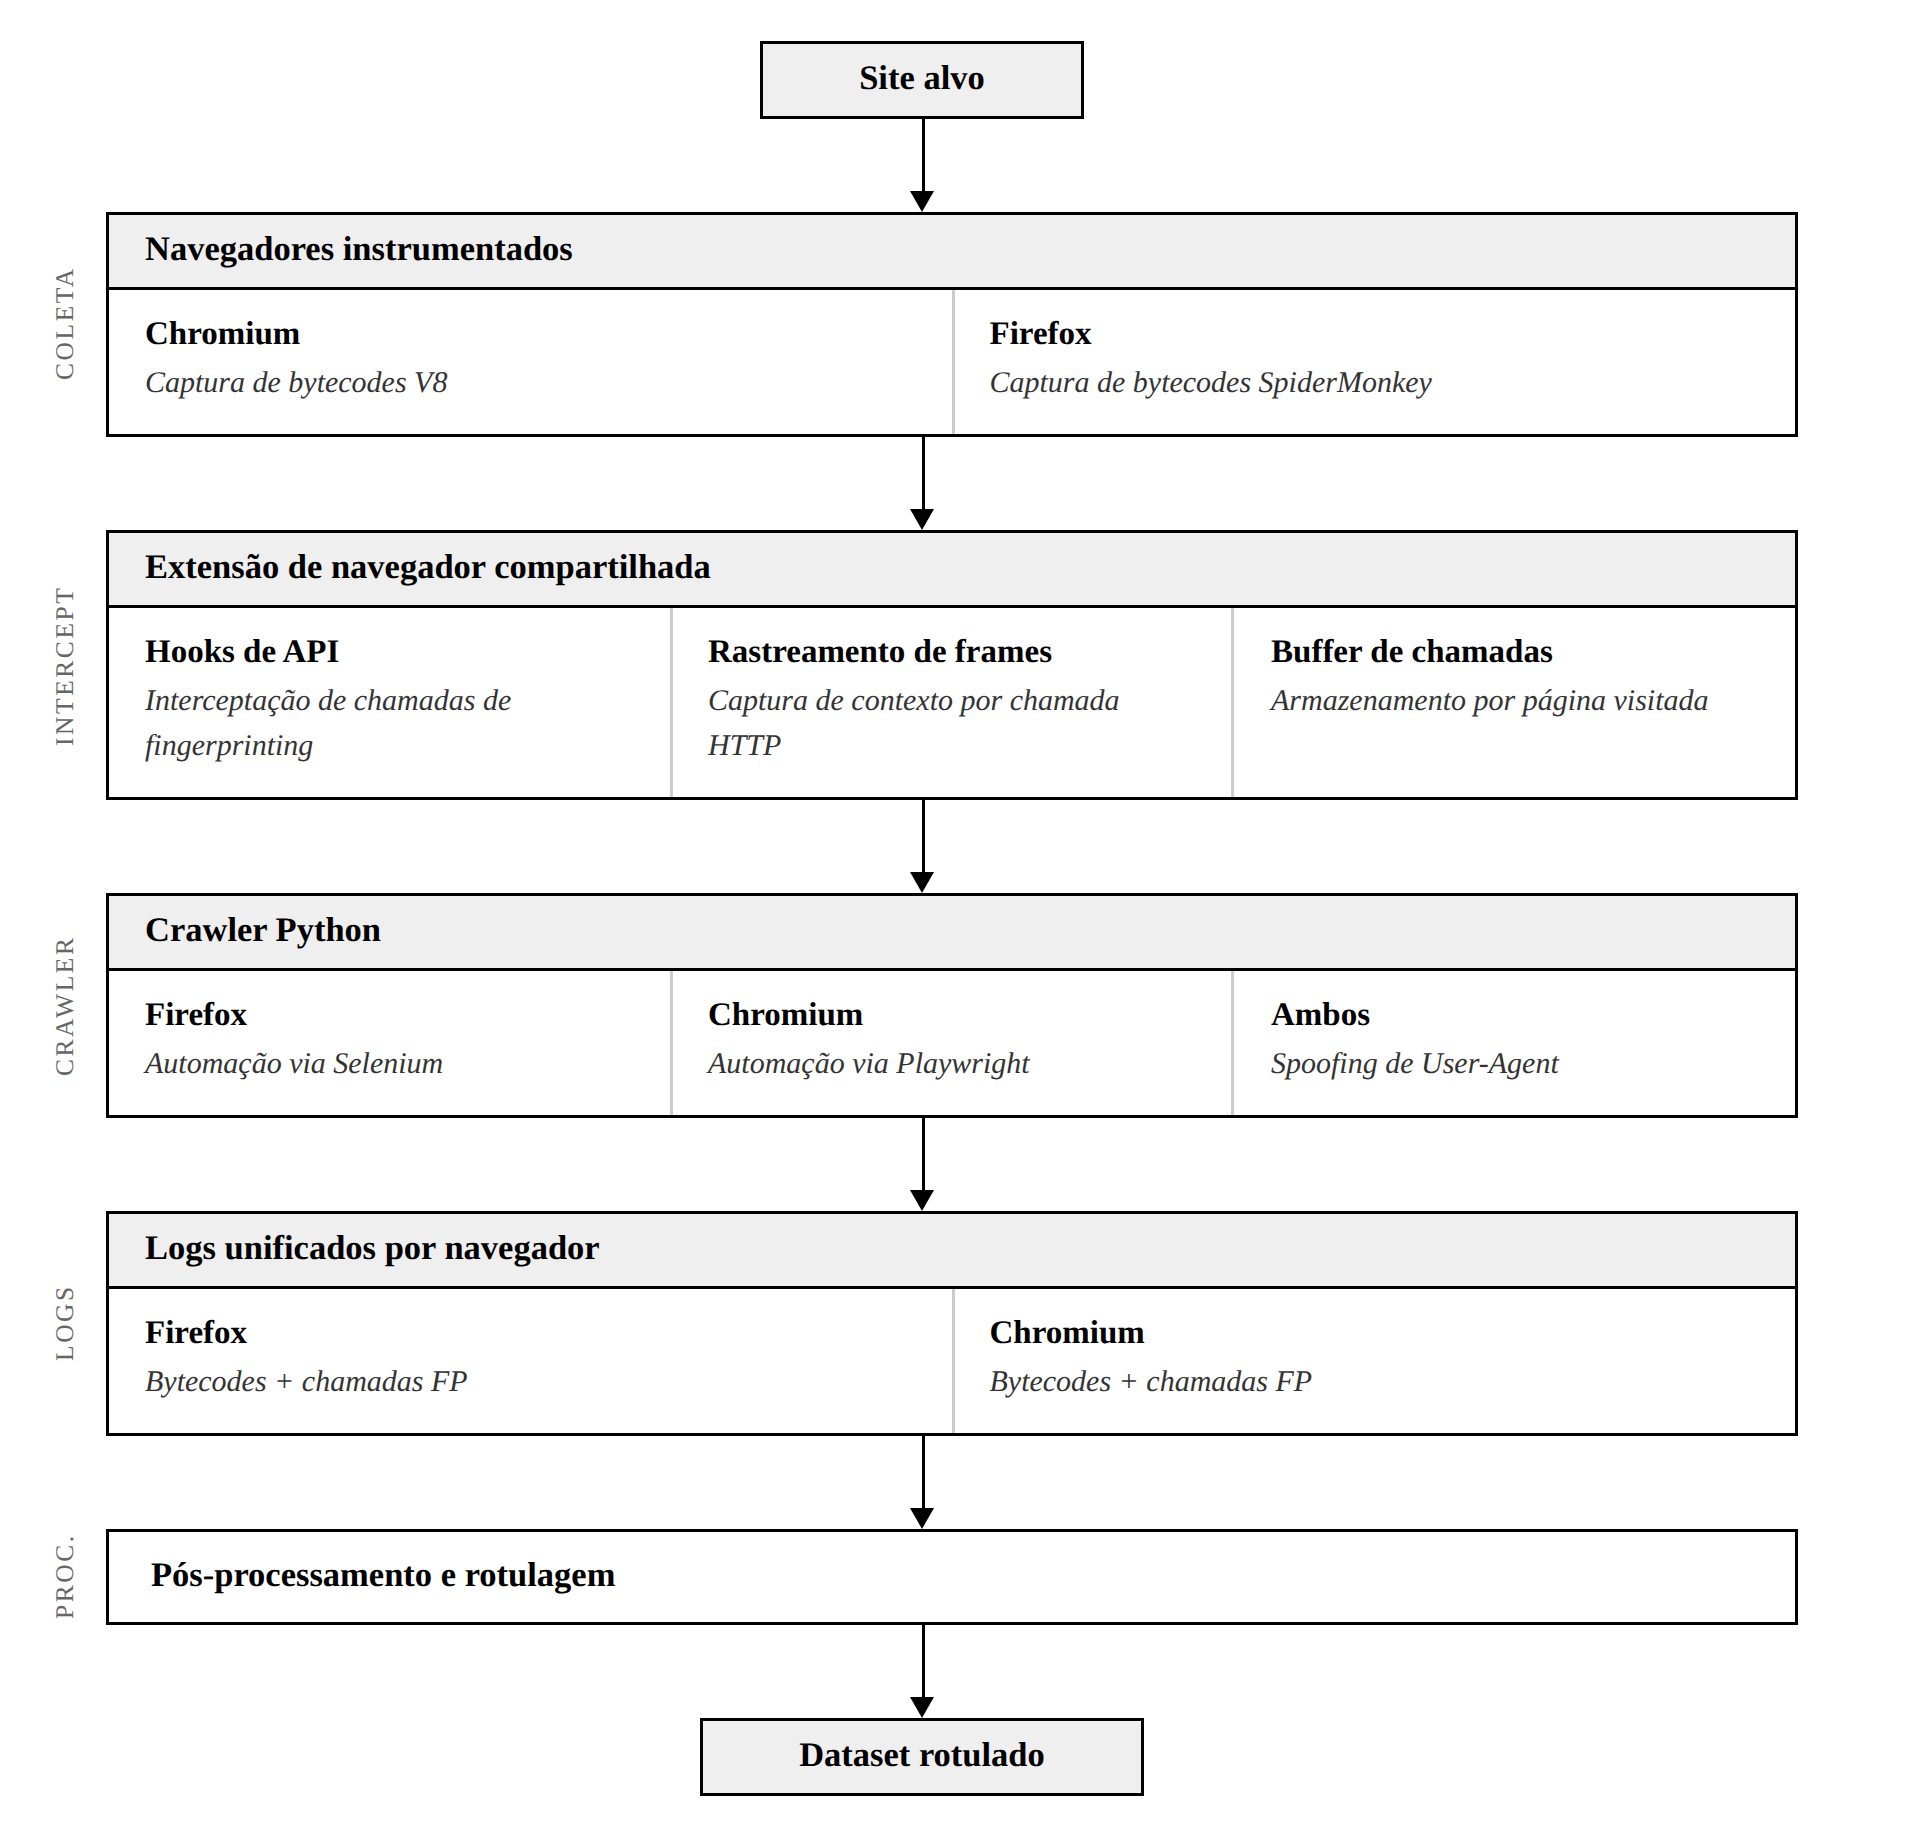
\includegraphics[width=\textwidth]{pipeline}
\fonte{Elaborada pelo autor.}
\end{figure}

O formato JSONL de bytecodes é unificado entre os dois navegadores, com os campos
\texttt{browser}, \texttt{injected\_id}, \texttt{script\_url}, \texttt{script\_id},
\texttt{function\_name} e \texttt{bytecodes} presentes em ambos. O campo
\texttt{injected\_id} possui semântica distinta nos dois motores e é descrito nas
seções seguintes.

%, , , , , , , , , , , , , , , , , , , --
\section{Instrumentação do V8}
\label{sec:v8}

A instrumentação é inserida no interpretador Ignition, invocada ao término
da compilação de cada função JavaScript. Para cada função, um identificador
estável é computado via hash FNV-1a de 64 bits sobre a combinação de URL do
script e posições de início/fim no código-fonte, garantindo reprodutibilidade
entre sessões. Funções sem script associado (built-ins e módulos internos) são
descartadas. Cada registro é emitido para o fluxo de erro padrão com o prefixo
\texttt{[V8Log]}, contendo identificador, URL, posições e sequência de bytecodes.
O código completo de instrumentação está no Apêndice~\ref{ap:instrumentacao}.

%, , , , , , , , , , , , , , , , , , , --
\section{Instrumentação do SpiderMonkey e injeção de ID para funções anônimas}
\label{sec:sm}

\subsection{Formato de emissão}
\label{sub:sm-formato}

A instrumentação do SpiderMonkey emite um bloco de texto por função compilada,
identificado pelo prefixo \texttt{[SpiderMonkey Log]}, com URL do script, nome da
função e sequência de bytecodes. O formato usa múltiplas linhas por registro,
ao contrário do JSON de linha única do V8. Um exemplo completo está no
Apêndice~\ref{ap:crawler-ext}.

\subsection{O problema das funções anônimas}
\label{sub:sm-anon}

Em bundles JavaScript minificados, a grande maioria das funções não possui
nome: \texttt{Function name} aparece como string vazia no log do SpiderMonkey. Sem
nome, não é possível ligar o registro de bytecodes a uma chamada de API capturada
pela extensão, o \texttt{Error.stack} expõe o nome da função chamadora, e uma
string vazia produz colisões massivas no join.

A solução implementada neste trabalho é a \textbf{injeção de identificador único
como \texttt{displayName}}: no código-fonte do SpiderMonkey, funções anônimas
recebem um nome sintético no formato \texttt{anon\_injected\_ID} no momento da
compilação, onde \texttt{ID} é um hash de 64 bits baseado em atributos da função
(URL do script e índice interno). Esse nome é armazenado como \texttt{displayName}
da função, que o motor do JavaScript propaga automaticamente para
\texttt{Error.stack} quando a função aparece na pilha de chamadas.

O efeito prático é que a extensão de navegador, ao capturar um \texttt{Error.stack}
durante uma chamada a \texttt{canvas.toDataURL}, enxerga o nome
\texttt{anon\_injected\_ID} na pilha, mesmo que a função não tenha nome no
código-fonte original, e o registra em \texttt{funcName}. O parser do
crawler encontra o registro de bytecodes com exatamente o mesmo
\texttt{function\_name}, e o join ocorre sem perda de dados.

Essa abordagem eliminou a perda de dados que afetava aproximadamente 38\% das
funções anônimas na versão anterior do pipeline, que tentava identificar funções
por posição no script.

\subsection{Parser do log SpiderMonkey}
\label{sub:sm-parser}

O crawler Firefox processa o log do geckodriver ao final de cada batch de
sites: identifica os blocos \texttt{[SpiderMonkey Log]}, descarta URLs internas
do Firefox, deduplica registros entre batches e converte o resultado para o
formato JSONL unificado. Detalhes estão no Apêndice~\ref{ap:instrumentacao}.

%, , , , , , , , , , , , , , , , , , , --
\section{Extensão de navegador: hooking de APIs e captura de pilha multi-frame}
\label{sec:extensao}

\subsection{Arquitetura e hooking de protótipos}
\label{sub:ext-arq}

A extensão compartilhada é uma extensão Manifest V3 carregada por ambos os
navegadores. Seu script de conteúdo é injetado antes de qualquer script do
site, garantindo que os hooks estejam ativos desde o início do carregamento da
página. A interceptação é feita por substituição de métodos nos protótipos das
APIs alvo; propriedades somente leitura são redefinidas com preservação dos
valores originais. Os detalhes de implementação estão no
Apêndice~\ref{ap:crawler-ext}.

As 32 APIs monitoradas estão listadas na Tabela~\ref{tab:apis}.

\begin{table}[htb]
\centering
\caption{APIs interceptadas pela extensão de navegador}
\label{tab:apis}
\begin{tabularx}{\linewidth}{l>{\raggedright\arraybackslash}X}
\toprule
\textbf{Categoria} & \textbf{Métodos / Propriedades interceptados} \\
\midrule
Canvas          & \texttt{toDataURL}, \texttt{getImageData}, \texttt{fillText}, \texttt{measureText}, \texttt{font} (setter), \texttt{save}, \texttt{restore} \\
OffscreenCanvas & \texttt{fillText}, \texttt{measureText}, \texttt{font} (setter) \\
Áudio           & \texttt{createOscillator}, \texttt{createDynamicsCompressor}, \texttt{startRendering}, \texttt{connect}, \texttt{copyFromChannel}, \texttt{getChannelData} \\
WebGL~1         & \texttt{getParameter}, \texttt{getSupportedExtensions} \\
WebGL~2         & \texttt{getParameter} \\
Tela            & \texttt{colorDepth}, \texttt{pixelDepth}, \texttt{width}, \texttt{height}, \texttt{availWidth} \\
Navigator       & \texttt{hardwareConcurrency}, \texttt{languages}, \texttt{platform}, \texttt{deviceMemory}, \texttt{maxTouchPoints} \\
WebRTC          & \texttt{createOffer}, \texttt{createDataChannel}, \texttt{setLocalDescription} \\
\bottomrule
\end{tabularx}
\fonte{Elaborada pelo autor.}
\end{table}

\subsection{Captura de pilha multi-frame}
\label{sub:ext-stack}

Para cada chamada de API interceptada, a extensão captura a pilha de chamadas
completa e registra todos os frames HTTP presentes, não apenas o chamador
imediato. Essa estratégia é necessária para que o pós-processador atribua
rótulos às funções orquestradoras que delegam chamadas de API para sub-rotinas
internas. Os detalhes de implementação, incluindo o tratamento de diferenças de
formato de stack trace entre V8 e SpiderMonkey, estão no
Apêndice~\ref{ap:crawler-ext}.

%, , , , , , , , , , , , , , , , , , , --
\section{Normalização de propriedades do Firefox}
\label{sec:normalizacao}

Uma condição necessária para o alinhamento cross-engine é que os sites web sirvam
o mesmo bundle JavaScript aos dois navegadores e que as bibliotecas de
fingerprinting executem os mesmos caminhos de código em ambos. Por padrão,
isso não ocorre: o Firefox expõe propriedades exclusivas que essas bibliotecas
detectam para selecionar implementações alternativas, ou para pular
completamente vetores como Canvas.

A extensão, executada em \texttt{document\_start}, realiza as seguintes
normalizações antes que qualquer script do site execute:

\textbf{Adições para simular Chromium:}
\begin{itemize}
  \item \texttt{window.chrome = \{ runtime: \{\} \}}, presente no Chromium,
    ausente no Firefox; a ausência é usada por bibliotecas como FingerprintJS para
    detectar Firefox.
  \item \texttt{navigator.vendor = 'Google Inc.'}, o Firefox retorna string
    vazia; o Chromium retorna \texttt{'Google Inc.'}.
\end{itemize}

\textbf{Remoções de propriedades exclusivas do Firefox:}
\begin{itemize}
  \item \texttt{navigator.buildID, navigator.globalPrivacyControl, navigator.oscpu}, presentes apenas no Firefox; usados como
    indicadores de motor pelo FingerprintJS e similares.
  \item \texttt{window.mozInnerScreenX}, \texttt{window.onmozfullscreenchange},
    \texttt{document.documentElement.style.MozAppearance}, propriedades
    prefixadas \texttt{moz}, detectadas por heurísticas de identificação de motor.
\end{itemize}

Além disso, o User-Agent é configurado no crawler Firefox para o valor
idêntico ao do Chromium~131 (string completa no Apêndice~\ref{ap:crawler-ext}).

O efeito combinado dessas normalizações é que sites que utilizam
\texttt{isFirefox()} ou verificações análogas para desviar o fluxo de coleta de
fingerprints passam a executar o mesmo código nos dois navegadores,
produzindo chamadas de API comparáveis entre sessões. Sem essas normalizações,
sites como os que utilizam FingerprintJS produzem zero chamadas à Canvas API no
Firefox.

%, , , , , , , , , , , , , , , , , , , --
\section{Crawlers}
\label{sec:crawlers}

Os dois crawlers visitam os 10.000 sites-alvo com Firefox e Chromium
instrumentados, emitindo logs no formato JSONL unificado. Ambos simulam
interação humana após o carregamento das páginas para ativar fingerprinting
condicionado a eventos, impõem timeout por site e são idempotentes,
permitindo retomada sem reprocessamento após falhas. Os detalhes de
implementação estão no Apêndice~\ref{ap:crawler-ext}.

%, , , , , , , , , , , , , , , , , , , --
\section{Estratégia de join: bytecodes <---> chamadas de API}
\label{sec:join}

O pós-processador liga cada registro de bytecodes ao conjunto de chamadas de
API observadas na mesma função, produzindo as colunas de rótulo multilabel do
dataset. A estratégia de join varia segundo o motor e o tipo
de função (Tabela~\ref{tab:join}).

\begin{table}[htb]
\centering
\caption{Estratégias de join por motor e tipo de função}
\label{tab:join}
\begin{tabularx}{\linewidth}{llX}
\toprule
\textbf{Motor} & \textbf{Tipo de função} & \textbf{Estratégia} \\
\midrule
Firefox (SM) & Nomeada & Join por nome da função \\
Firefox (SM) & Anônima & Join por nome: ID injetado (\texttt{anon\_injected\_ID}) propaga-se para o call stack \\
Chromium (V8) & Nomeada & Join por (URL do script, nome da função) \\
Chromium (V8) & Anônima & Join por posição: (linha, coluna) convertido a offset de caractere \\
\bottomrule
\end{tabularx}
\fonte{Elaborada pelo autor.}
\end{table}

Para o Chromium, o offset de caractere é determinado a partir de linha e
coluna; o intervalo mais interno é selecionado para resolver sobreposições de
funções aninhadas. As heurísticas de rotulagem multilabel que determinam as
categorias de fingerprinting a partir do padrão de chamadas de API observado
são descritas em detalhe no Capítulo~\ref{cap:dataset}.

% ============================================================
%  Capítulo 4 — Dataset
% ============================================================
\chapter{DATASET}
\label{cap:dataset}

\section{Configuração do crawl}
\label{sec:crawl-config}

\subsection{Seleção de sites}
\label{sub:sitios}

Os sites-alvo são os 10.000 primeiros da lista Tranco \cite{lepochat2019}, uma
classificação de popularidade de domínios baseada em múltiplas listas de tráfego
agregadas semanalmente. A Tranco é preferida em relação à lista Alexa por ser
reprodutível (cada versão é identificada por data e pode ser consultada
retroativamente) e por filtrar domínios de infraestrutura e CDN que distorcem
classificações baseadas em DNS puro.

O mesmo conjunto de 10.000 URLs é visitado pelos dois crawlers:
Firefox/SpiderMonkey e Chromium/V8. Isso garante que cada site contribua com dois
registros de bytecodes, um por motor, para o mesmo conjunto de chamadas de
API, tornando o dataset intrinsecamente cross-engine.

\subsection{Parâmetros de visita}
\label{sub:params}

Cada site é visitado uma única vez por navegador, com os seguintes parâmetros:

\begin{table}[htb]
\centering
\caption{Parâmetros de visita por crawler}
\label{tab:params}
\begin{tabularx}{\linewidth}{lXX}
\toprule
\textbf{Parâmetro} & \textbf{Firefox} & \textbf{Chromium} \\
\midrule
Timeout de carregamento             & 15\,s & 15\,s \\
Watchdog por site                  & 60\,s & 60\,s \\
Comportamento pós-carregamento      & scroll em 5 posições + digitação & scroll em 5 posições + digitação \\
Espera extra após FP detectado      & 2\,s  & 2\,s \\
Reinício do navegador               & a cada 30 sites & a cada 10 sites \\
\bottomrule
\end{tabularx}
\fonte{Elaborada pelo autor.}
\end{table}

O comportamento de scroll e digitação simula interação humana, ativando
event listeners de sites que iniciam a coleta de fingerprint apenas
após interação do usuário. O reinício periódico do Firefox controla o tamanho do
arquivo de log do geckodriver, que seria processado integralmente ao final de cada
batch. O reinício do Chromium foi feito com maior frequência por conta do maior consumo de memória acumulada entre sessões.

\subsection{Idempotência e retomada}
\label{sub:idempotencia}

Ambos os crawlers são idempotentes: registram URLs concluídas em arquivos
de progresso e retomam a partir da última URL pendente em caso de
reinicialização. Bytecodes são escritos
incrementalmente no arquivo JSONL de saída; chamadas de API são appended ao
arquivo correspondente após cada visita.

%, , , , , , , , , , , , , , , , , , , --
%, , , , , , , , , , , , , , , , , , , --
\section{Estatísticas do dataset}
\label{sec:stats}

\subsection{Dataset rotulado bruto}
\label{sub:stats-bruto}

Após o crawl completo dos 10.000 sites com ambos os navegadores e o
processamento pelo pós-processador, o dataset rotulado bruto apresenta
as seguintes características:

\begin{table}[htb]
\centering
\caption{Estatísticas do dataset rotulado bruto}
\label{tab:stats-bruto}
\begin{tabular}{ll}
\toprule
\textbf{Métrica} & \textbf{Valor} \\
\midrule
Funções totais                                            & 68.008.403 \\
Funções de fingerprinting (\texttt{is\_fp = True})        & 37.644 (0,055\%) \\
Funções não-FP                                            & 67.970.759 (99,945\%) \\
Tamanho do arquivo (Parquet, zstd)                        & 5,43~GB \\
\bottomrule
\end{tabular}

\fonte{Elaborada pelo autor.}
\end{table}

A proporção de 0,055\% de funções positivas é característica de crawls de
alta escala: a vasta maioria das funções JavaScript de uma página serve a
propósitos de interface, roteamento, gerenciamento de estado ou analytics, não
de fingerprinting. Esse nível extremo de desbalanceamento motiva a
estratégia de amostragem descrita na Seção~\ref{sec:amostragem}.

\subsection{Distribuição por categoria}
\label{sub:stats-cats}

Os rótulos multilabel não são mutuamente exclusivos: uma função pode ser
classificada em mais de uma categoria se suas chamadas de API satisfizerem os
critérios de múltiplas heurísticas. A Figura~\ref{fig:cats} apresenta a distribuição de funções por categoria relativo ao total de funções FP.

\begin{figure}[htb]
\centering
\caption{Distribuição de funções de fingerprinting por categoria (categorias não exclusivas).}
\label{fig:cats}
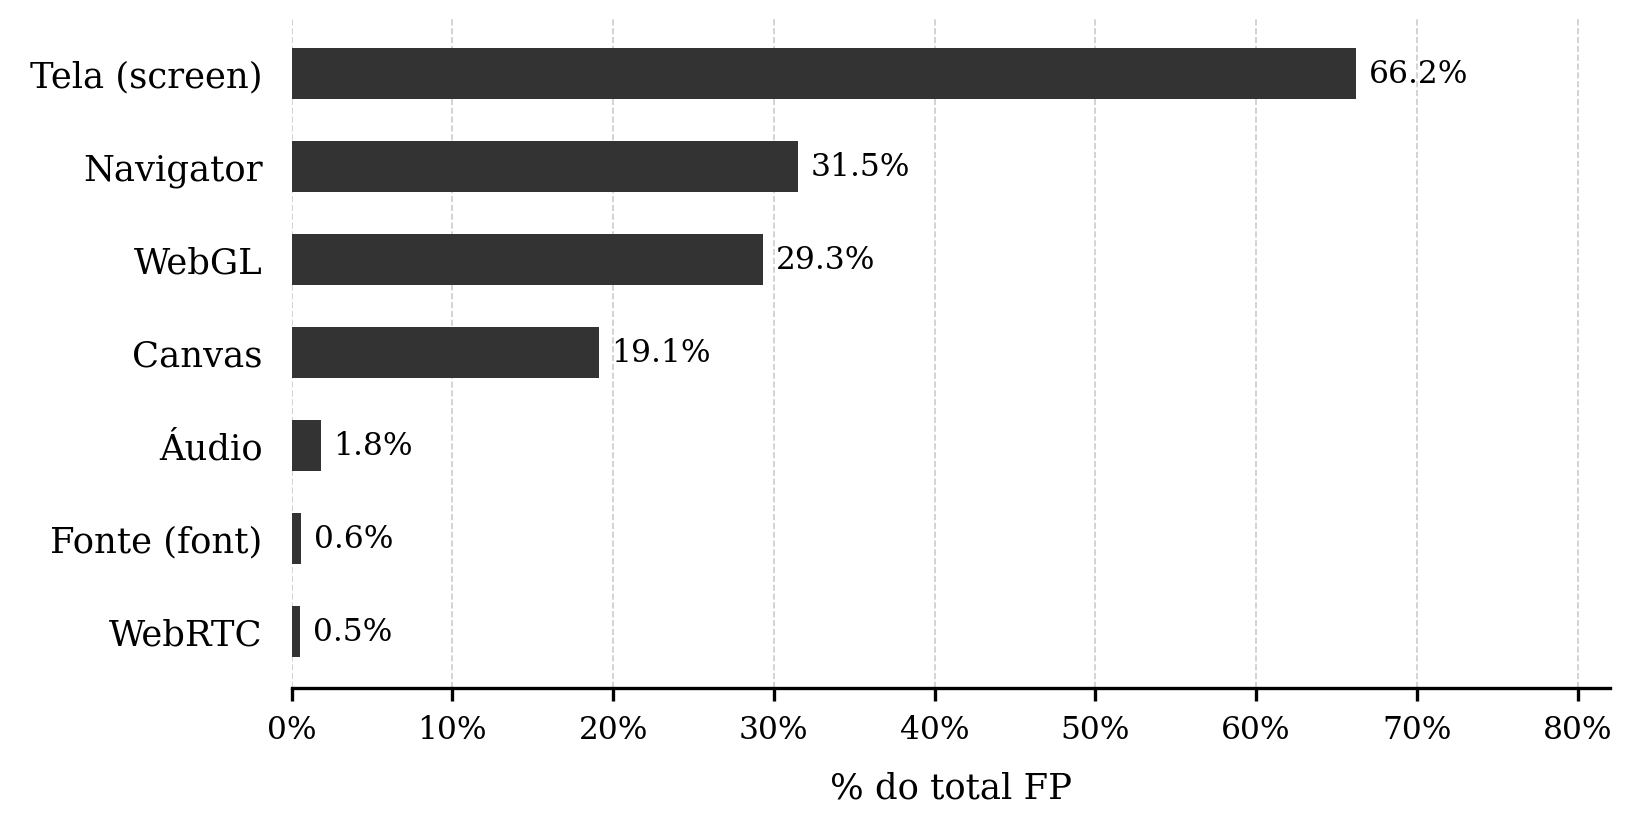
\includegraphics[width=0.82\linewidth]{fig_category_distribution}

\fonte{Elaborada pelo autor.}
\end{figure}

A Figura~\ref{fig:cats} ilustra graficamente essa distribuição. A assimetria é de
duas ordens de magnitude entre as categorias mais comuns (Tela, WebGL, Navigator)
e as mais raras (WebRTC, Fonte).
Categorias como Tela e Navigator são coletadas por praticamente qualquer biblioteca
de fingerprinting, enquanto WebRTC e Fonte aparecem apenas em
implementações mais agressivas, presentes em uma minoria dos sites do Top~10k.
Essa assimetria tem implicações diretas para o desempenho dos classificadores
multilabel, discutidas no Capítulo~\ref{cap:discussao}.

%, , , , , , , , , , , , , , , , , , , --
\section{Heurísticas ByteDefender para atribuição de rótulos multilabel}
\label{sec:heuristicas}

A atribuição de rótulos não é feita por inspeção manual nem por palavras-chave no
nome da função: as funções de fingerprinting têm nomes arbitrários,
especialmente em bundles minificados. Em vez disso, o pós-processador
implementa heurísticas baseadas no padrão de chamadas de API observado durante
a execução, seguindo a metodologia do ByteDefender \cite{nikkhahbahrami2025}.

Para cada função, o pós-processador agrega o conjunto de APIs chamadas, o
comprimento máximo do argumento de \texttt{fillText}, o número de chamadas a
\texttt{measureText}, o número de valores distintos do setter \texttt{font}, o
número de chamadas WebGL que expõem parâmetros de fabricante/renderizador e o
número de propriedades distintas de \texttt{navigator} acessadas. Com base
nesses agregados, cada heurística é avaliada como uma expressão booleana:

\textbf{Canvas.} Presença simultânea de \texttt{canvas.toDataURL} e
\texttt{canvas.fillText} com argumento de comprimento mínimo 10, combinada com
ausência de \texttt{canvas.save} e \texttt{canvas.restore}. Os critérios negativos
discriminam uso de canvas para renderização de interface, que frequentemente envolve
save/restore, do uso para extração de fingerprint, que não necessita dessas
operações.

\textbf{Áudio.} Presença simultânea de \texttt{audio.\allowbreak createOscillator},
\texttt{audio.\allowbreak createDynamicsCompressor}, \texttt{audio.\allowbreak startRendering},
\texttt{audio.\allowbreak connect} e pelo menos um entre \texttt{audio.\allowbreak getChannelData} e
\texttt{audio.\allowbreak copyFromChannel}. O padrão completo (oscilar, comprimir, renderizar offline, conectar e extrair o resultado) é a assinatura canônica da técnica de audio fingerprinting.

\textbf{WebRTC.} Presença de \texttt{webrtc.setLocalDescription} combinada com
\texttt{webrtc.createOffer} ou \texttt{webrtc.createDataChannel}. A negociação de
candidatos ICE, que expõe IPs locais, requer obrigatoriamente
\texttt{setLocalDescription}.

\textbf{Fonte.} Pelo menos 20 chamadas a \texttt{canvas.measureText} e mais de 20
valores distintos do setter \texttt{canvas.font}. A enumeração de fontes requer a
medição das dimensões de texto em dezenas de famílias tipográficas, daí os
limiares elevados.

\textbf{WebGL.} Pelo menos uma chamada a \texttt{webgl.getParameter} com um
parâmetro que exponha informações do fabricante ou do renderizador da GPU
(\texttt{RENDERER}, \texttt{VENDOR} ou constantes de extensão equivalentes).

\textbf{Tela.} Presença de \texttt{screen.colorDepth} ou
\texttt{screen.pixelDepth}, combinada com pelo menos uma entre
\texttt{screen.width}, \texttt{screen.height} e \texttt{screen.availWidth}. O
acesso isolado a dimensões de tela é comum em código responsivo legítimo; a
combinação com profundidade de cor é o indicador de fingerprinting.

\textbf{Navigator.} Pelo menos 3 propriedades distintas de \texttt{navigator}
acessadas dentre as monitoradas (\texttt{hardwareConcurrency}, \texttt{languages},
\texttt{platform}, \texttt{deviceMemory}, \texttt{maxTouchPoints}). O acesso a
uma ou duas propriedades pode ocorrer legitimamente; o acesso a três ou mais indica
coleta sistemática de perfil de hardware.

%, , , , , , , , , , , , , , , , , , , --
\section{Limpeza de ruído}
\label{sec:limpeza}

\subsection{Origem do ruído}
\label{sub:ruido-origem}

O dataset bruto contém tokens espúrios provenientes de dois mecanismos:

\textbf{Artefatos de cabeçalho de log.} A separação entre o prefixo de log e o
conteúdo JSON é feita por parsing de texto simples. Em casos de quebra de linha
inesperada, por exemplo, quando o sistema operacional interrompe uma escrita em
stderr, o prefixo \texttt{[V8Log]} ou \texttt{[SpiderMonkey Log]} pode
aparecer embutido dentro da string de bytecodes, gerando tokens como
\texttt{[SpiderMonkey}, \texttt{Log]} ou \texttt{Return[V8Log]}.

\textbf{Tokens truncados.} O geckodriver impõe um limite de comprimento por linha de
log do SpiderMonkey; o sistema operacional pode interromper escritas longas em stderr
para o V8. Funções com sequências de bytecodes muito longas têm as últimas sequências
truncadas, produzindo tokens parciais como \texttt{GetNam} (em vez de
\texttt{GetNamedProperty} no SpiderMonkey) ou \texttt{LdaConst} (em vez de
\texttt{LdaConstant} no V8) ou caracteres isolados como \texttt{S}, \texttt{C},
\texttt{L}.

\textbf{Normalização de formato.} O SpiderMonkey emite bytecodes com espaço após
a vírgula (\texttt{"A, B, C"}), enquanto o V8 não usa espaço (\texttt{"A,B,C"}).
O módulo de limpeza normaliza para o formato sem espaço.

\subsection{Regra de filtragem}
\label{sub:ruido-filtro}

Um token é considerado válido se e somente se corresponde à expressão regular:

\begin{lstlisting}[language={}]
^[A-Za-z][A-Za-z0-9_]{1,}$
\end{lstlisting}

A regra exige início com letra, comprimento mínimo de 2 caracteres e composição
exclusivamente alfanumérica com sublinhados. Tokens com colchetes, tokens de um
caractere e tokens truncados são descartados. Linhas cujos bytecodes ficam
completamente vazios após a filtragem são removidas do dataset.

\subsection{Resultado da limpeza}
\label{sub:ruido-resultado}

\begin{table}[htb]
\centering
\caption{Resultado da limpeza de ruído}
\label{tab:limpeza}
\begin{tabular}{ll}
\toprule
\textbf{Métrica} & \textbf{Valor} \\
\midrule
Linhas processadas                                            & 68.008.403 \\
Taxa de ruído de tokens                                       & 1,17\% \\
Arquivo de saída (Parquet limpo, zstd) & 5,10~GB \\
\bottomrule
\end{tabular}

\fonte{Elaborada pelo autor.}
\end{table}

A taxa de ruído de 1,17\% confirma que a maioria das sequências de bytecodes está
íntegra. Os tokens removidos concentram-se em um subconjunto pequeno de funções
com bytecodes muito longos (afetados pelo truncamento do geckodriver para o
SpiderMonkey ou por interrupções de escrita em stderr para o V8) e em funções
cujos scripts foram carregados durante reinicializações do navegador.

%, , , , , , , , , , , , , , , , , , , --
\section{Amostra de treinamento}
\label{sec:amostragem}

\subsection{Problema de escala e desbalanceamento}
\label{sub:escala}

O dataset limpo contém 68 milhões de funções. Carregar todas as sequências de
tokens em memória para treinamento de classificadores baseados em TF-IDF é
inviável: a matriz TF-IDF em formato denso (68M $\times$ 4.723~features de
bigrams, em \texttt{float32}) ocuparia aproximadamente 1,3~TB de RAM. Além disso, o
desbalanceamento de 1:1.806 (FP:não-FP) inviabiliza o treinamento direto sem
estratégia de amostragem.

\subsection{Sampler em dois passes}
\label{sub:sampler}

O amostrador opera em dois passes sobre o arquivo Parquet:

\textbf{Passo~1, estimativa de FP.} Um em cada 50 grupos de linhas (row
groups) do arquivo Parquet é lido, carregando apenas a coluna \texttt{is\_fp}. O
número de funções FP no corpus completo é estimado por extrapolação linear:

\begin{equation}
\hat{n}_{\text{FP}} = n_{\text{FP}}^{\text{amostra}} \times
\frac{N_{\text{total}}}{N_{\text{amostra}}}
\end{equation}

\textbf{Passo~2, coleta completa.} O arquivo é lido integralmente, grupo por
grupo. Todas as funções FP são retidas. Funções não-FP são incluídas com
probabilidade de Bernoulli:

\begin{equation}
p_{\text{neg}} = \min\!\left(1{,}0,\;
\frac{r \cdot \hat{n}_{\text{FP}}}{N_{\text{total}} - \hat{n}_{\text{FP}}}\right)
\end{equation}

onde $r$ é a razão de negativos por positivo ($r = 10$). Com
$\hat{n}_{\text{FP}} \approx 48.822$ (estimativa do passo~1, consideravelmente
superior ao valor real de 37.644, sobreestimativa de $\approx$30\% decorrente
da distribuição não-uniforme de funções FP entre os grupos de linhas do arquivo
Parquet), $p_{\text{neg}} \approx 0{,}72\%$.

\subsection{Características da amostra}
\label{sub:amostra-stats}

A Tabela~\ref{tab:amostra} apresenta a composição da amostra resultante do
processo de dois passes. Todos os 37.644 exemplos FP são retidos; os negativos são
subamostrados com razão $r = 10$, produzindo uma amostra gerenciável em memória
com desbalanceamento efetivo de 1:13.

\begin{table}[htb]
\centering
\caption{Composição da amostra de treinamento}
\label{tab:amostra}
\begin{tabular}{ll}
\toprule
\textbf{Métrica} & \textbf{Valor} \\
\midrule
Funções FP na amostra    &  37.644 \\
Funções não-FP na amostra & 488.166 \\
Total da amostra         & 525.810 \\
Razão FP:não-FP efetiva  & 1:13,0 \\
\bottomrule
\end{tabular}

\fonte{Elaborada pelo autor.}
\end{table}

\subsection{Divisão treino/teste}
\label{sub:split}

A amostra é dividida em 80\% para treinamento e 20\% para teste com estratificação
pela coluna \texttt{is\_fp} e semente aleatória~42. A estratificação garante que a
proporção de positivos seja idêntica em ambas as partições.

\begin{table}[htb]
\centering
\caption{Divisão treino/teste}
\label{tab:split}
\begin{tabular}{lrr}
\toprule
\textbf{Partição} & \textbf{Linhas totais} & \textbf{Funções FP} \\
\midrule
Treinamento & 420.648 & 30.115 \\
Teste       & 105.162 &  7.529 \\
\bottomrule
\end{tabular}

\fonte{Elaborada pelo autor.}
\end{table}

A mesma divisão, gerada com a mesma semente e a mesma ordem de leitura do
Parquet, é utilizada por todos os classificadores (RF, LightGBM, SVM, BiLSTM e
Transformer), garantindo comparabilidade direta entre os resultados reportados no
Capítulo~\ref{cap:experimentos}.

% ============================================================
%  Capítulo 5 — Representação Intermediária Cross-Engine
% ============================================================
\chapter{REPRESENTAÇÃO INTERMEDIÁRIA CROSS-ENGINE}
\label{cap:ir}

\section{Motivação: vocabulários disjuntos entre V8 e SpiderMonkey}
\label{sec:ir-motivacao}

A detecção de fingerprinting baseada em bytecodes pressupõe que o
classificador opere sobre um espaço de features compartilhado entre os motores que
se deseja suportar. Essa condição não é satisfeita por nenhum conjunto de opcodes
nativo: os conjuntos de instrução do V8 (Ignition) e do SpiderMonkey são definidos
independentemente por suas equipes de desenvolvimento e não possuem nomes em comum.

Além da diferença nominal, os dois motores adotam arquiteturas de máquina virtual
distintas. O V8 utiliza uma \textbf{máquina de registradores com acumulador
implícito}: cada instrução opera sobre o acumulador e, opcionalmente, sobre
registradores explicitamente nomeados. O SpiderMonkey utiliza uma \textbf{máquina
de pilha}: operandos são empilhados explicitamente antes de cada instrução e o
resultado é depositado no topo da pilha. Uma operação aritmética que o V8 codifica
em uma única instrução, por exemplo, \texttt{Add r1} (soma o registrador
\texttt{r1} ao acumulador), requer três instruções no SpiderMonkey:
\texttt{GetLocal 0; GetLocal 1; Add}. Isso implica que a mesma função JavaScript
produz sequências de bytecodes de comprimentos diferentes e com tokens distintos
nos dois motores.

A Tabela~\ref{tab:opcodes-divergencia} ilustra a divergência para um trecho
representativo de código de fingerprinting, leitura de
\texttt{navigator.hardwareConcurrency}:

\begin{table}[htb]
\centering
\caption{Opcodes para \texttt{let x = navigator.hardwareConcurrency}}
\label{tab:opcodes-divergencia}
\begin{tabular}{lll}
\toprule
\textbf{Passo semântico} & \textbf{V8 (Ignition)} & \textbf{SpiderMonkey} \\
\midrule
Carregar \texttt{navigator}           & \texttt{LdaGlobal}       & \texttt{GetGName} \\
Ler \texttt{.hardwareConcurrency}     & \texttt{GetNamedProperty} & \texttt{GetProp} \\
Armazenar em variável local           & \texttt{Star0}            & \texttt{SetLocal} \\
\bottomrule
\end{tabular}
\fonte{Elaborada pelo autor.}
\end{table}

Treinar um classificador TF-IDF diretamente sobre bytecodes brutos de um motor e
aplicá-lo ao outro é equivalente a usar vocabulários completamente disjuntos:
nenhum feature do modelo de origem existe no espaço de features do destino. Os
experimentos de transferência zero-shot (Capítulo~\ref{cap:experimentos}) confirmam
empiricamente essa intuição, com F1 entre 0,149 e 0,180.

A solução proposta neste trabalho é uma \textbf{representação intermediária
cross-engine (RI)}: um vocabulário fixo de tokens abstratos que substituem os
opcodes nativos de ambos os motores, preservando as distinções semânticas relevantes
para a tarefa de classificação de fingerprinting. O mesmo trecho acima,
traduzido para a RI, torna-se \texttt{LOAD\_GLOBAL, GET\_NAMED\_PROP, STORE\_LOCAL}
em ambos os motores.

%, , , , , , , , , , , , , , , , , , , --
\section{Metodologia dos micro-scripts}
\label{sec:micro}

\subsection{Motivação para a abordagem empírica}
\label{sub:micro-motivacao}

A correspondência entre opcodes dos dois motores não pode ser derivada
automaticamente a partir de suas especificações: não existe documentação formal que
mapeie instruções V8 para instruções SpiderMonkey. A única fonte de verdade é a
observação empírica: executar o mesmo código JavaScript nos dois motores
instrumentados e comparar as sequências de bytecodes produzidas.

Para que o mapeamento seja exaustivo e auditável, é necessário que os scripts de
teste cubram sistematicamente as construções JavaScript relevantes para
fingerprinting, uma por vez, de forma que a correspondência entre opcodes
possa ser estabelecida por inspeção direta da saída.

\subsection{Conjunto de micro-scripts}
\label{sub:micro-conjunto}

Foram elaborados 27 micro-scripts JavaScript, cada um
exercitando uma construção isolada. A Tabela~\ref{tab:micro} lista os scripts e as
construções cobertas.


\begin{longtable}{l p{0.55\linewidth}}
\caption{Micro-scripts e construções JavaScript cobertas}
\label{tab:micro} \\
\toprule
\textbf{Script} & \textbf{Construção} \\
\midrule
\endfirsthead
\toprule
\textbf{Script} & \textbf{Construção} \\
\midrule
\endhead
\bottomrule
\endlastfoot
\texttt{01\_literals.js}       & Literais numéricos, booleanos, \texttt{null}, \texttt{undefined} \\
\texttt{02\_local\_vars.js}    & Leitura e escrita de variáveis locais \\
\texttt{03\_global\_vars.js}   & Leitura e escrita de variáveis globais \\
\texttt{04\_closure\_vars.js}  & Leitura e escrita de variáveis de closure (upvalues) \\
\texttt{05\_property\_read.js} & Leitura de propriedade nomeada (\texttt{obj.prop}) \\
\texttt{06\_property\_write.js}& Escrita de propriedade nomeada (\texttt{obj.prop = v}) \\
\texttt{07\_keyed\_read.js}    & Leitura de propriedade indexada (\texttt{obj[key]}) \\
\texttt{08\_keyed\_write.js}   & Escrita de propriedade indexada (\texttt{obj[key] = v}) \\
\texttt{09\_arithmetic.js}     & Operações aritméticas (\texttt{+}, \texttt{-}, \texttt{*}, \texttt{/}, \texttt{\%}, \texttt{**}) \\
\texttt{10\_bitwise.js}        & Operações bitwise (\texttt{|}, \texttt{\&}, \texttt{\textasciicircum}, \texttt{<<}, \texttt{>>}, \texttt{>>>}) \\
\texttt{11\_unary.js}          & Operadores unários (\texttt{-}, \texttt{\textasciitilde}, \texttt{!}, \texttt{++}, \texttt{--}) \\
\texttt{12\_comparisons.js}    & Comparações (\texttt{==}, \texttt{===}, \texttt{<}, \texttt{>}, \texttt{<=}, \texttt{>=}) \\
\texttt{13\_typeof.js}         & Operador \texttt{typeof} \\
\texttt{14\_conditional.js}    & Desvios condicionais (\texttt{if}/\texttt{else}, operador ternário) \\
\texttt{15\_loops.js}          & Laços (\texttt{for}, \texttt{while}, \texttt{do...while}) \\
\texttt{16\_logical.js}        & Operadores lógicos de curto-circuito (\texttt{\&\&}, \texttt{||}, \texttt{??}) \\
\texttt{17\_method\_call.js}   & Chamada de método (\texttt{obj.method(args)}) \\
\texttt{18\_function\_call.js} & Chamada de função pura (\texttt{func(args)}) \\
\texttt{19\_constructor.js}    & Construção de objeto (\texttt{new Class(args)}) \\
\texttt{20\_return.js}         & Instrução \texttt{return} \\
\texttt{21\_closure\_create.js}& Criação de closure \\
\texttt{22\_object\_literal.js}& Literal de objeto (\texttt{\{ k: v \}}) \\
\texttt{23\_array\_literal.js} & Literal de array (\texttt{[a, b, c]}) \\
\texttt{24\_try\_catch.js}     & Bloco \texttt{try}/\texttt{catch}/\texttt{throw} \\
\texttt{25\_type\_coercion.js} & Coerções de tipo (\texttt{Number()}, \texttt{String()}, \texttt{Boolean()}) \\
\texttt{26\_instanceof.js}     & Operador \texttt{instanceof} \\
\texttt{27\_string\_concat.js} & Concatenação de strings \\
\end{longtable}

As construções escolhidas cobrem intencionalmente os padrões observados no topo da
lista de importância de features (Capítulo~\ref{cap:experimentos}): acesso a
propriedades (scripts 05--08), chamadas de método e função (17, 18), variáveis de
closure (04, 21) e desvios condicionais com \texttt{try/catch} (14, 24).

\subsection{Execução pareada e alinhamento}
\label{sub:micro-exec}

Cada micro-script é executado nos dois navegadores instrumentados por um script
de automação. Para cada execução, captura-se a sequência de bytecodes emitida
pelo motor para a função principal do micro-script e salva-se o resultado com
as sequências de cada motor.

O alinhamento é feito em duas etapas:

\begin{enumerate}
\item \textbf{Alinhamento manual.} Para cada par
  \texttt{(v8\_bytecodes, sm\_bytecodes)}, os opcodes são inspecionados
  visualmente e agrupados por correspondência semântica. A diferença de
  arquitetura (registrador vs. pilha) exige mapeamentos de cardinalidade
  N:1 ou 1:N em alguns casos, por exemplo, um único \texttt{Add} do V8 pode
  corresponder a \texttt{GetLocal; GetLocal; Add} do SpiderMonkey, mas todos os
  três são mapeados para o mesmo token de RI \texttt{BINARY\_ADD}.

\item \textbf{Validação estatística.} O validador aplica o mapeamento estático
  ao corpus de micro-scripts e calcula a cobertura dos opcodes observados.
  Mapeamentos que deixam opcodes frequentes sem correspondência são revisados
  até que a cobertura do corpus de micro-scripts atinja 100\%.
\end{enumerate}

A Figura~\ref{fig:ir-metodologia} sintetiza essa metodologia.

\begin{figure}[htb]
\centering
\caption{Metodologia de construção da representação intermediária cross-engine}
\label{fig:ir-metodologia}
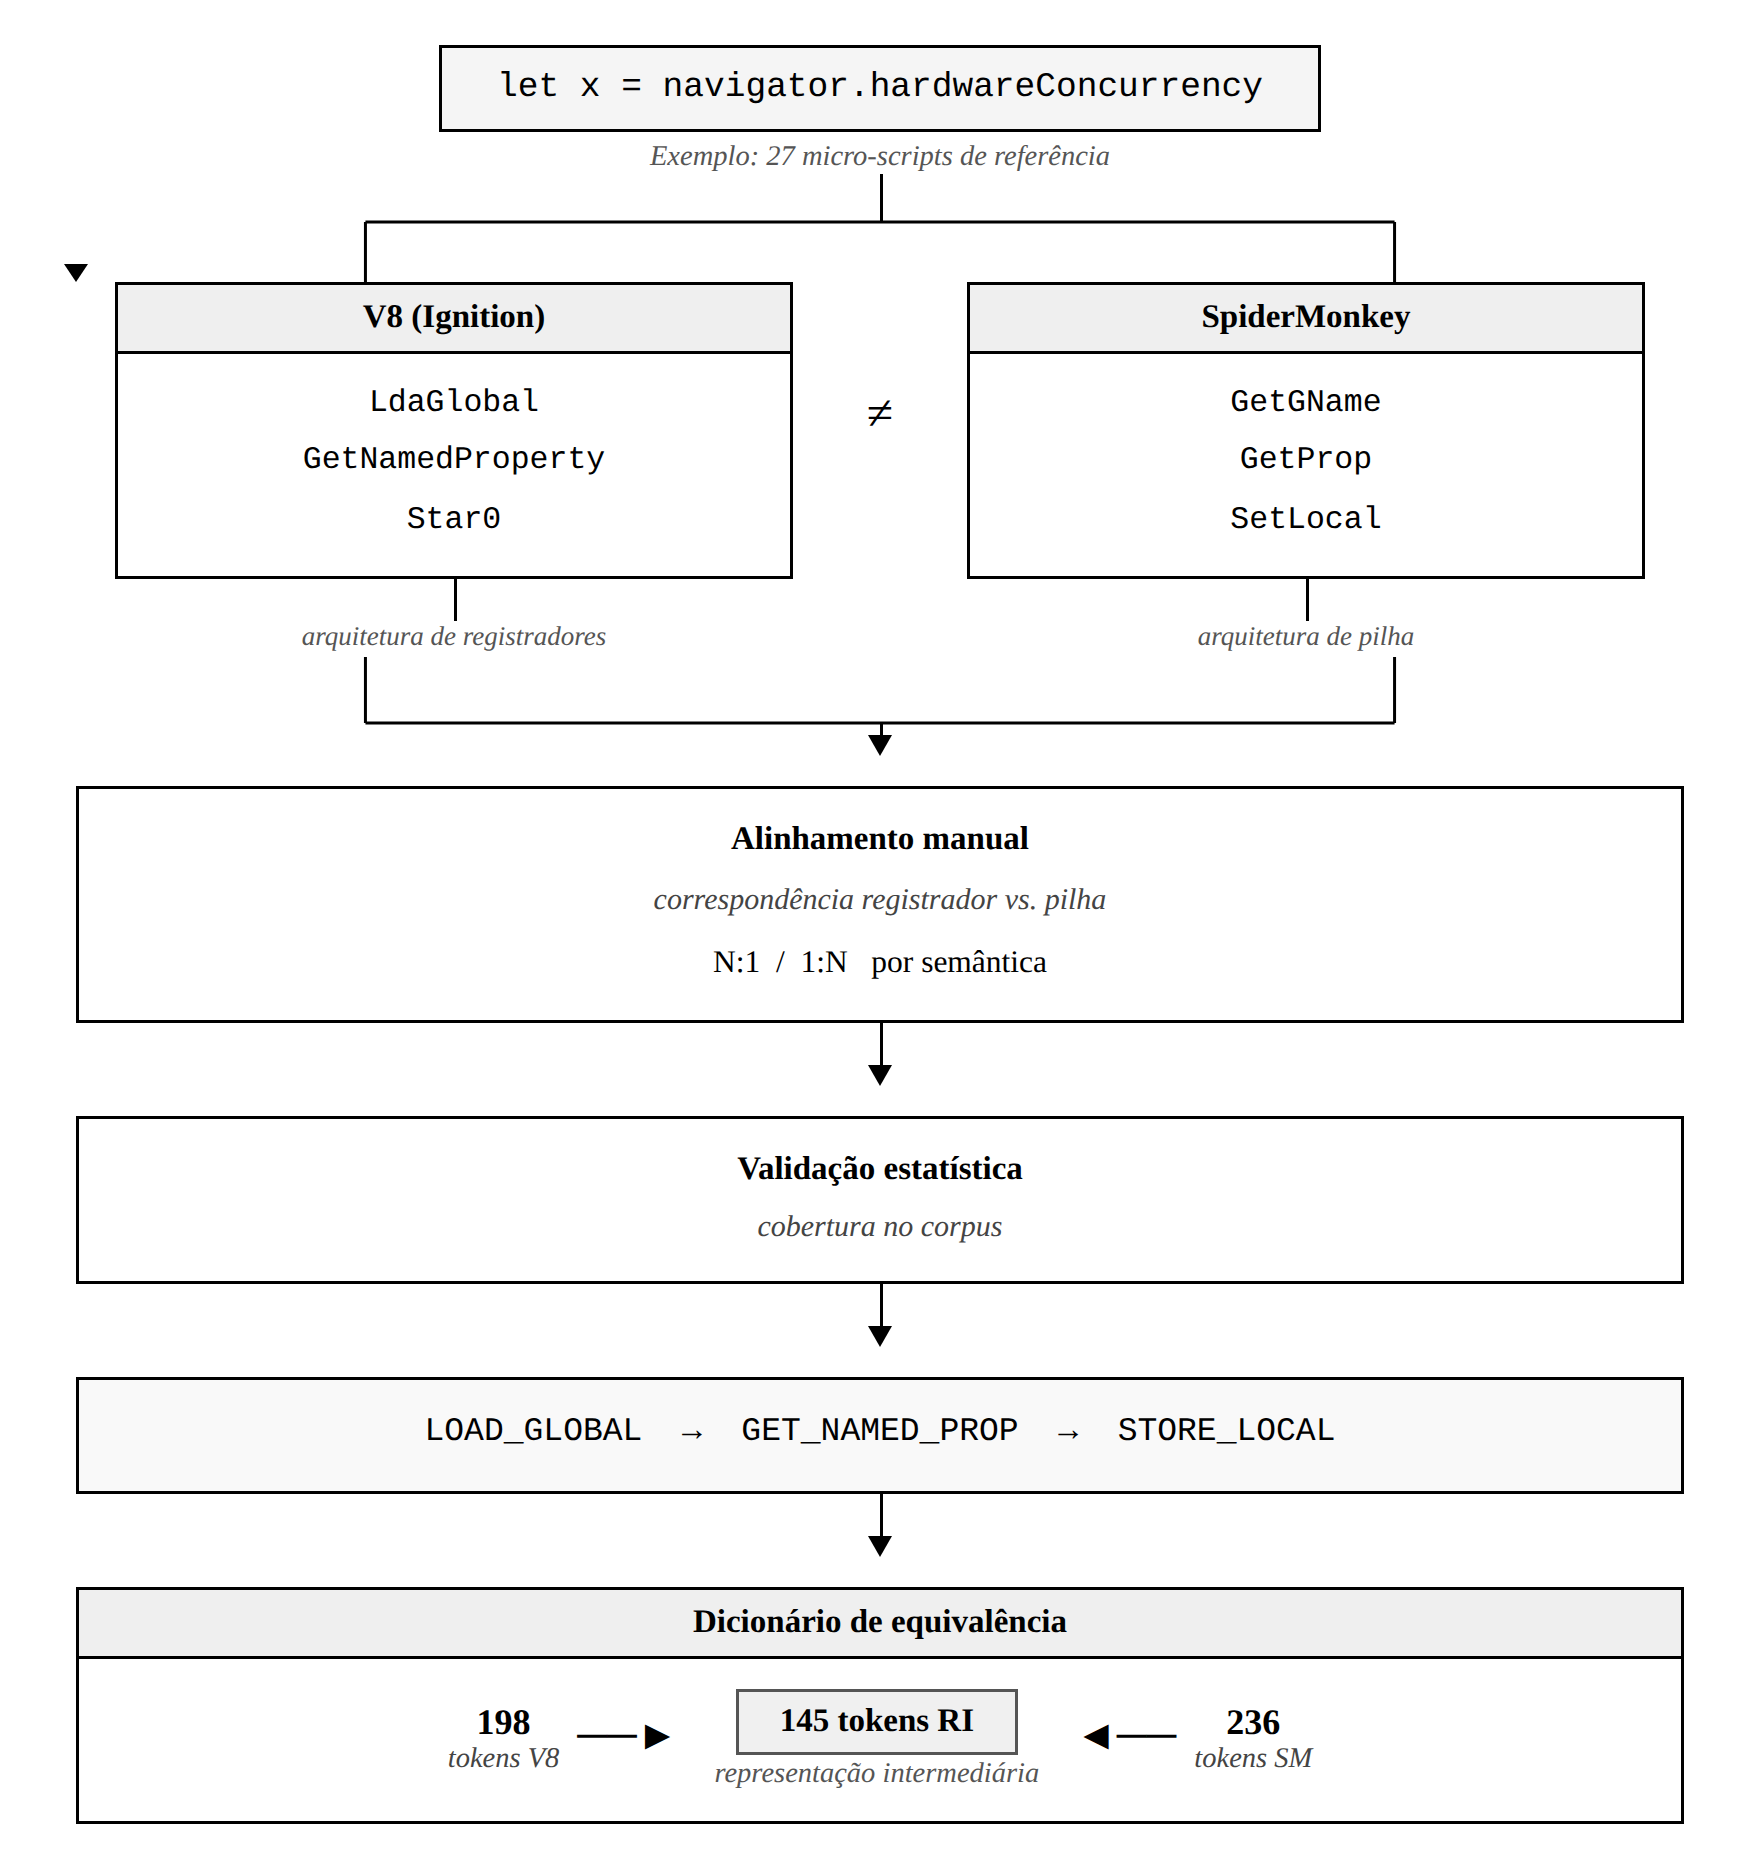
\includegraphics[width=0.92\linewidth]{fig_ir_methodology}

\fonte{Elaborada pelo autor.}
\end{figure}

%, , , , , , , , , , , , , , , , , , , --
\section{Dicionário de equivalência}
\label{sec:dict}

\subsection{Estrutura e dimensões}
\label{sub:dict-estrutura}

O dicionário de equivalência contém dois mapeamentos planos: \texttt{v8\_to\_ir}
(198 entradas) e \texttt{sm\_to\_ir}
(236 entradas), ambos mapeando para o mesmo conjunto de 145 tokens de RI. O número
maior de entradas no lado SpiderMonkey reflete a granularidade mais alta do
conjunto de instrução de pilha: construções que o V8 codifica em poucos opcodes
correspondem a múltiplos opcodes especializados no SpiderMonkey sob o mesmo token de RI.
Por exemplo, o token \texttt{LOAD\_INT} cobre apenas \texttt{LdaZero} e \texttt{LdaSmi}
no V8, mas seis variantes no SpiderMonkey (\texttt{Zero}, \texttt{One}, \texttt{Int8},
\texttt{Int32}, \texttt{Uint16}, \texttt{Uint24}).

A Tabela~\ref{tab:dict-exemplos} apresenta exemplos representativos do dicionário
para as categorias de maior importância discriminativa.

\begin{table}[htb]
\centering
\caption{Exemplos de mapeamentos por categoria no dicionário de equivalência}
\label{tab:dict-exemplos}
\begin{tabularx}{\linewidth}{l>{\raggedright\arraybackslash}X>{\raggedright\arraybackslash}X}
\toprule
\textbf{Token de RI} & \textbf{Opcodes V8 mapeados} & \textbf{Opcodes SM mapeados} \\
\midrule
\texttt{GET\_KEYED\_PROP}   & \texttt{GetKeyedProperty}, \texttt{GetEnumeratedKeyedProperty} & \texttt{GetElem} \\
\texttt{GET\_NAMED\_PROP}   & \texttt{GetNamedProperty}, \texttt{GetNamedPropertyFromSuper} & \texttt{GetProp} \\
\texttt{LOAD\_CLOSURE\_VAR} & \texttt{LdaContextSlot}, \ldots\ (13 variantes) & \texttt{GetAliasedVar} \\
\texttt{CALL\_FUNC}         & --- & \texttt{Call}, \texttt{CallIgnoresRv}, \ldots \\
\texttt{CALL\_FUNC\_N}      & \texttt{CallUndefinedReceiver}, \texttt{CallAnyReceiver}, \texttt{CallWithSpread} & --- \\
\texttt{CALL\_METHOD\_N}    & \texttt{CallProperty} & --- \\
\texttt{BINARY\_ADD}        & \texttt{Add}, \texttt{AddSmi} & \texttt{Add} \\
\texttt{STORE\_LOCAL}       & \texttt{Star}, \texttt{Star0}--\texttt{Star15}, \texttt{Mov} & \texttt{SetLocal} \\
\texttt{TRY\_START}         & ---                                                     & \texttt{Try} \\
\bottomrule
\end{tabularx}
\fonte{Elaborada pelo autor.}
\end{table}

O V8 possui variantes \texttt{*Smi} para operações aritméticas e bit a bit que são
caminhos rápidos especializados para inteiros pequenos (small integers).
Essas variantes não têm equivalente direto no SpiderMonkey e são mapeadas para o
mesmo token de RI que a instrução genérica correspondente.

\subsection{Cobertura no corpus real}
\label{sub:dict-cobertura}

A cobertura foi medida sobre o corpus completo de 68 milhões de funções,
que contém 4,41 bilhões de tokens de bytecodes nativos distribuídos entre os
dois motores. A cobertura de 99,82\% é calculada sobre o corpus misto; o valor
é reportado por motor na tabela abaixo como a fração dos tokens daquele motor
que possui mapeamento no dicionário.

\begin{table}[htb]
\centering
\caption{Cobertura do dicionário de equivalência no corpus real}
\label{tab:cobertura}
\begin{tabular}{lrr}
\toprule
\textbf{Métrica} & \textbf{V8} & \textbf{SpiderMonkey} \\
\midrule
Mapeamentos no dicionário           & 198    & 236    \\
Cobertura de tokens (\% do total)   & 99,82\% & 99,82\% \\
Tokens não mapeados $\to$ \texttt{<UNK>} & $\approx$0,18\% & $\approx$0,18\% \\
\bottomrule
\end{tabular}
\fonte{Elaborada pelo autor.}
\end{table}

Os tokens não mapeados ($\approx$0,18\%) correspondem a opcodes específicos de
versões recentes do V8 e do SpiderMonkey não cobertos pelo conjunto de 27
micro-scripts, como variantes de instruções de feedback de tipo e opcodes
introduzidos após a construção do dicionário. As instruções de gerador/assíncrono e
de módulo ES têm mapeamentos explícitos no dicionário (ver Apêndice~\ref{ap:ir-dict},
seção \textit{Generators, async e miscelânea}) e não contribuem para o
\texttt{<UNK>}. Dois tokens de RI nunca aparecem no corpus real, \texttt{SCOPE\_INIT} e \texttt{WIDE\_PREFIX};
os 143 restantes reduzem-se a \textbf{136 tokens ativos} após filtragem por frequência
mínima (\texttt{min\_df}) nos conjuntos de treinamento amostrados.

%, , , , , , , , , , , , , , , , , , , --
\section{Pipeline de tradução do dataset}
\label{sec:traducao}

O pipeline de tradução lê o dataset limpo um grupo de linhas (row group) por
vez (o arquivo possui 401 grupos com $\approx$170 mil linhas cada) e
aplica a tradução token a token, produzindo o dataset traduzido.

Para cada função, o campo \texttt{browser} determina qual mapeamento usar
(\texttt{sm\_to\_ir} para Firefox ou \texttt{v8\_to\_ir} para Chromium). Os
bytecodes separados por vírgula são traduzidos token a token; tokens ausentes no
dicionário recebem o símbolo especial \texttt{<UNK>}. O delimitador muda de
vírgula para espaço na sequência de RI, alinhando-se ao formato esperado pelo
TF-IDF e pelo FastText. A coluna de bytecodes é substituída pela sequência de
tokens de RI; todas as demais colunas são preservadas.

O processamento em streaming mantém o pico de memória em $\approx$4~GB
(dominado pelo grupo de linhas corrente mais os buffers de escrita PyArrow),
viabilizando a execução em máquinas com 16~GB de RAM sem armazenamento temporário
em disco.

%, , , , , , , , , , , , , , , , , , , --
\section{Embeddings FastText}
\label{sec:embeddings}

\subsection{Construção do corpus de treinamento}
\label{sub:corpus}

O corpus de treinamento é gerado iterando todas as 68 milhões de sequências
de tokens de RI do dataset traduzido. Duas situações de borda são tratadas:

\textbf{Sequências muito curtas.} Funções com menos de 2 tokens de RI (811
stubs com apenas \texttt{RETURN}) são descartadas: não possuem janela de
contexto válida para o algoritmo Skip-gram e produziriam gradientes inválidos.

\textbf{Sequências muito longas.} Funções com mais de 512 tokens são divididas em
fragmentos não sobrepostos de 512 tokens cada, sem descarte de tokens. A divisão é
semanticamente equivalente à sequência completa para o Skip-gram, que opera sobre
janelas de contexto locais de $\pm$5 posições, a co-ocorrência entre tokens
distantes não é capturada de qualquer forma. A alternativa de truncar em 512
descartaria silenciosamente tokens de fingerprinting que aparecem no final
de funções longas.

\subsection{Decisões críticas de treinamento}
\label{sub:fasttext-decisoes}

\textbf{Algoritmo: Skip-gram, não CBOW.} O CBOW (Word2Vec) foi treinado e
descartado. Com um vocabulário fechado de 145 tokens, o amostrador negativo do CBOW
escolhe com alta frequência o próprio token positivo como amostra negativa, gerando
gradientes contraditórios. O resultado foi colapso de vetores: 5 vetores com
NaN/Inf, 28 vetores com norma zero, e coerência semântica de categoria $-0{,}010$
(pior que aleatório). O Skip-gram inverte o problema de predição, prevê o
contexto a partir da palavra central, e produz gradientes bem definidos mesmo
com vocabulário pequeno.

\textbf{Subsampling desativado ($t = 0{,}0$).} O parâmetro $t$ controla a taxa de
descarte de tokens de alta frequência durante o treinamento. O valor padrão
$t = 1 \times 10^{-4}$ descarta tokens cujas frequências relativas excedem o
limiar. Com apenas 145 tipos no vocabulário, todos os tokens qualificam-se como
``alta frequência'' sob esse critério, e virtualmente todo o sinal de treinamento é
eliminado nas primeiras iterações. Definir $t = 0{,}0$ desativa o subsampling
completamente, que é o comportamento correto para um vocabulário fechado desta
magnitude.

\textbf{\texttt{minCount = 1}.} Para garantir que todos os 145 tokens de RI
recebam vetores mesmo que apareçam raramente no corpus, o limiar mínimo de
frequência é fixado em~1.

\textbf{Hiperparâmetros de treinamento:}

\begin{table}[htb]
\centering
\caption{Hiperparâmetros do modelo FastText Skip-gram}
\label{tab:fasttext-hp}
\begin{tabular}{ll}
\toprule
\textbf{Parâmetro} & \textbf{Valor} \\
\midrule
Algoritmo            & Skip-gram \\
Dimensão             & 128 \\
Épocas               & 5 \\
Janela de contexto   & 5 \\
\texttt{minCount}    & 1 \\
Subsampling $t$      & 0,0 \\
Threads       & 4 \\
Chunk size    & 512 tokens \\
\bottomrule
\end{tabular}

\fonte{Elaborada pelo autor.}
\end{table}

\subsection{Avaliação dos embeddings}
\label{sub:fasttext-eval}

\textbf{Saúde dos vetores.} O modelo FastText resultante não apresenta vetores
degenerados: 0 vetores NaN/Inf, 0 vetores de norma zero, norma média de 0,0061, e
similaridade de cosseno média entre pares de 0,017, indicando que o espaço
vetorial está bem distribuído e não colapsado.

\textbf{Coerência semântica de categoria.} O avaliador de embeddings computa, para cada categoria de opcode, a
similaridade de cosseno média intra-categoria (pares de tokens na mesma
categoria) e inter-categoria (pares entre categorias distintas). O
gap positivo confirma que tokens semanticamente relacionados estão mais
próximos entre si do que de tokens de outras categorias.

\begin{table}[htb]
\centering
\caption{Coerência por categoria de token de RI (FastText Skip-gram)}
\label{tab:coerencia}
\begin{tabular}{lrrr}
\toprule
\textbf{Categoria} & \textbf{Intra} & \textbf{Inter} & \textbf{Gap} \\
\midrule
\texttt{PROP\_GET} & 0,505 &  0,047 & \textbf{+0,458} \\
\texttt{BINARY}    & 0,478 & $-0{,}004$ & \textbf{+0,482} \\
\texttt{CREATE}    & 0,436 &  0,005 & \textbf{+0,431} \\
\texttt{CALL}      & 0,355 &  0,005 & \textbf{+0,350} \\
\texttt{LOAD}      & 0,328 &  0,004 & \textbf{+0,324} \\
\texttt{BITWISE}   & 0,331 &  0,010 & \textbf{+0,321} \\
\texttt{PROP\_SET} & 0,286 &  0,033 & \textbf{+0,253} \\
\texttt{STORE}     & 0,251 &  0,007 & \textbf{+0,244} \\
\texttt{CMP}       & 0,201 & $-0{,}003$ & \textbf{+0,204} \\
\texttt{UNARY}     & 0,142 &  0,015 & \textbf{+0,127} \\
\texttt{JMP}       & 0,054 &  0,001 & \textbf{+0,053} \\
\texttt{COERCE}    & 0,052 &  0,004 & \textbf{+0,048} \\
\texttt{CONTROL}   & $-0{,}006$ & $-0{,}010$ & \textbf{+0,004} \\
\midrule
\textbf{GERAL}     & \textbf{0,245} & \textbf{0,008} & \textbf{+0,237} \\
\bottomrule
\end{tabular}

\fonte{Elaborada pelo autor.}
\end{table}

As categorias \texttt{PROP\_GET} e \texttt{BINARY} apresentam os maiores
gaps, refletindo a alta co-ocorrência contextual entre tokens de acesso a
propriedades (típicos de código de fingerprinting) e entre operadores
aritméticos. A categoria \texttt{CONTROL}, que agrupa \texttt{RETURN},
\texttt{POP}, \texttt{THROW} e \texttt{SWAP}, apresenta gap próximo de
zero por ser semanticamente heterogênea: esses tokens não compartilham contexto de
co-ocorrência, e o modelo corretamente os representa com vetores dissimilares.

\textbf{Independência de motor.} O modelo foi treinado sobre o corpus misto
(Firefox + Chromium) sem rótulo de motor. Qualquer estrutura de agrupamento no
espaço vetorial é portanto intrinsecamente cross-engine: quando \texttt{BINARY\_ADD}
aparece em uma sequência SpiderMonkey e em uma sequência V8, ambas as ocorrências
contribuem para o mesmo vetor. O gap de coerência geral de +0,237 confirma
que o modelo aprendeu estrutura semântica a partir desse sinal combinado.

% ============================================================
%  Capítulo 6 — Experimentos e Resultados
% ============================================================
\chapter{EXPERIMENTOS E RESULTADOS}
\label{cap:experimentos}

\section{Configuração experimental}
\label{sec:exp-config}

\subsection{Features}
\label{sub:exp-features}

Todos os classificadores utilizam exclusivamente a coluna \texttt{ir\_tokens} do
dataset traduzido como entrada. Nenhuma feature de metadados é utilizada, nome
da função, URL do script, identificador de motor ou posição no código-fonte são
deliberadamente excluídos. Esse isolamento garante que os resultados meçam a
capacidade discriminativa dos bytecodes em si, sem dependência de informações de
contexto que podem não estar disponíveis em cenários de implantação.

A representação de entrada varia por família de modelos, como demonstrado na Tabela~\ref{tab:features}.

\begin{table}[htb]
\centering
\caption{Representação de entrada por família de modelos}
\label{tab:features}
\begin{tabular}{l p{6cm} l}
\toprule
\textbf{Família} & \textbf{Representação} & \textbf{Dimensão} \\
\midrule
RF, SVM, LightGBM & TF-IDF esparso sobre tokens de RI & 136 / 4.723 / 50.631 \\
Transformer (v.1)  & Embeddings FastText 128-dim fixos, seq.\ até 512 tokens & 128 por posição \\
Transformer (v.2)  & Embeddings treináveis 128-dim, seq.\ até 512 tokens & 128 por posição \\
\bottomrule
\end{tabular}

\fonte{Elaborada pelo autor.}
\end{table}

\subsection{Divisão treino/teste}
\label{sub:exp-split}

Os experimentos binários e multilabel utilizam a divisão descrita no
Capítulo~\ref{cap:dataset} (Tabela~\ref{tab:split}: 30.115~FP treino, 7.529~FP
teste). O experimento de modelo conjunto cross-engine
(Seção~\ref{sec:crossengine}) usa uma amostra combinada de ambos os motores
sobre o mesmo conjunto de sites, cujos totais de FP são maiores por incluir
registros independentes de cada motor (Tabela~\ref{tab:split-exp}). O experimento
de transferência zero-shot (Seção~\ref{sub:zeroshot}) usa subconjuntos por motor
do dataset, separados por engine antes da amostragem. A estratificação é feita sobre \texttt{is\_fp} em todos os
casos.

\begin{table}[htb]
\centering
\caption{Divisão treino/teste: experimento cross-engine (modelo conjunto)}
\label{tab:split-exp}
{\footnotesize
Os totais de funções FP (33.087 treino, 8.272 teste) correspondem à amostra do
experimento cross-engine e excedem os 37.644 reportados no
Capítulo~\ref{cap:dataset} por incluir registros independentes de ambos os
motores coletados sobre o mesmo conjunto de sites. O número total de linhas
(525.810) é mantido igual à divisão padrão por sub-amostragem proporcional
dos negativos.
}

\bigskip
\begin{tabular}{lrr}
\toprule
\textbf{Partição} & \textbf{Linhas} & \textbf{FP} \\
\midrule
Treino & 420.648 & 33.087 \\
Teste  & 105.162 &  8.272 \\
\bottomrule
\end{tabular}

\fonte{Elaborada pelo autor.}
\end{table}

\subsection{Métricas}
\label{sub:exp-metricas}

Para a tarefa binária (\texttt{is\_fp}), reportam-se precisão, revocação e F1
sobre a classe positiva após ajuste de limiar (threshold tuning) no conjunto
de teste. O limiar é varrido em passos de 0,05 entre 0 e 1; o valor que maximiza o
F1 é selecionado. Para modelos com limiar padrão (RF), o limiar 0,50 é mantido.

Para a tarefa multilabel, reporta-se o F1 por rótulo e o macro-F1 (média não
ponderada entre os sete rótulos). O macro-F1 penaliza igualmente rótulos raros e
comuns, refletindo a dificuldade total da tarefa.

Para os experimentos cross-engine, reportam-se precisão, revocação e F1 por motor,
mais a média ponderada pelo suporte FP de cada motor.

\subsection{Hiperparâmetros dos modelos principais}
\label{sub:exp-hp}

\textbf{Random Forest (binário):} 200 árvores, balanceamento por subamostragem
por árvore (\textit{balanced\_subsample}), mínimo de 5 amostras por folha.

\textbf{LightGBM (binário):} 500 estimadores, taxa de aprendizado 0,05, 127
folhas por árvore, balanceamento automático de classes, subamostragem de 80\%
de linhas e colunas. Variante com contexto iterativo (iter.~2 e~3): 1.000
estimadores, razão de negativos por positivo $r = 7$.

Hiperparâmetros dos modelos adicionais (SVM, BiLSTM, Transformer, variantes
multilabel) são descritos na Seção~\ref{sec:adicionais}.

\subsection{Ambiente computacional}
\label{sub:exp-ambiente}

Os experimentos com LightGBM, Random Forest, SVM e o benchmark de inferência
foram executados em um notebook com processador Intel Core i7-12700H (20
threads), 16~GB de RAM, sob Fedora Linux~43. O treinamento do Transformer foi
realizado no cluster SLURM \textit{blaise} (PCAD/UFRGS), equipado com 4
GPUs Tesla P100-SXM2.

%, , , , , , , , , , , , , , , , , , , --
\section{Modelo base: LightGBM com bigrams}
\label{sec:baseline}

A Tabela~\ref{tab:bin} e a Figura~\ref{fig:f1-progressao} apresentam os resultados
da linha principal, do piso de unigrams à inferência iterativa com contexto de
script, permitindo acompanhar cada passo de ganho antes de introduzir o seguinte. O modelo oracle
(F1~=~0,928), que usa rótulos reais como features de contexto e não é implantável,
é discutido separadamente na Seção~\ref{sec:oracle}.

\begin{table}[htb]
\centering
\caption{Classificadores binários, linha principal (\texttt{is\_fp})}
\label{tab:bin}
{\footnotesize
Divisão 80/20 estratificada, semente~42. Dataset: 68M funções, 37.644 FP.
$\dagger$ByteDefender: valor reportado sobre bytecodes brutos V8, motor único.
$\P$Inferência iterativa sem rótulos oracle: contagens previstas em três limiares
($p{>}0{,}30$; $p{>}0{,}50$; $p{>}0{,}70$) e tamanho de script, recomputadas a
cada iteração. As variantes iter.~2 e iter.~3 ($\P$) usam $r = 7$; a variante de
duas passagens usa $r = 10$. O conjunto de treinamento menor de iter.~2 e iter.~3
(com $r = 7$) reduz o número de bigramas TF-IDF retidos acima da frequência mínima,
explicando a contagem de features inferior (4.574) em relação à variante de duas
passagens (4.726, treinada com $r = 10$).
}
\bigskip
{\small
\begin{tabularx}{\linewidth}{p{3.2cm}|X|r|r|r|r|l}
\toprule
\textbf{Modelo} & \textbf{Features} & \textbf{\# feat.} & \textbf{P} & \textbf{R} & \textbf{F1} & \textbf{Limiar} \\
\midrule
RF (unigrams)
  & TF-IDF unigrams
  &    136 & 0,834 & 0,835 & 0,834 & 0,50 \\[2pt]
LightGBM (bigrams)
  & TF-IDF bigrams
  &  4.723 & 0,888 & 0,802 & 0,843 & 0,80 \\[2pt]
LightGBM (trigrams)
  & TF-IDF trigrams
  & 50.631 & 0,885 & 0,809 & 0,845 & 0,80 \\[2pt]
LightGBM + densidade
  & TF-IDF bigrams + densidade de script
  &  4.724 & 0,883 & 0,825 & 0,853 & 0,80 \\[2pt]
LightGBM + duas passagens$\P$
  & + dens.\ + contagem FP prev.\ + tam.\
  &  4.726 & 0,901 & 0,848 & 0,874 & 0,80 \\[2pt]
LightGBM + iter.\ 2$\P$
  & + dens.\ + 3 cont.\ limiares + tam.\
  &  4.574 & 0,917 & 0,886 & 0,901 & 0,70 \\[2pt]
\textbf{LightGBM + iter.\ 3}$\P$
  & \textbf{idem iter.\ 2}
  & \textbf{4.574} & \textbf{0,934} & \textbf{0,876} & \textbf{0,904} & \textbf{0,80} \\[2pt]
ByteDefender$\dagger$ (motor único)
  & Bytecodes brutos V8
  & --- & --- & --- & $\approx$0,950 & --- \\
\bottomrule
\end{tabularx}
}% end \small
\fonte{Elaborada pelo autor.}
\end{table}

\begin{figure}[htb]
\centering
\caption{Progressão do F1 binário: do modelo base à inferência iterativa}
\label{fig:f1-progressao}
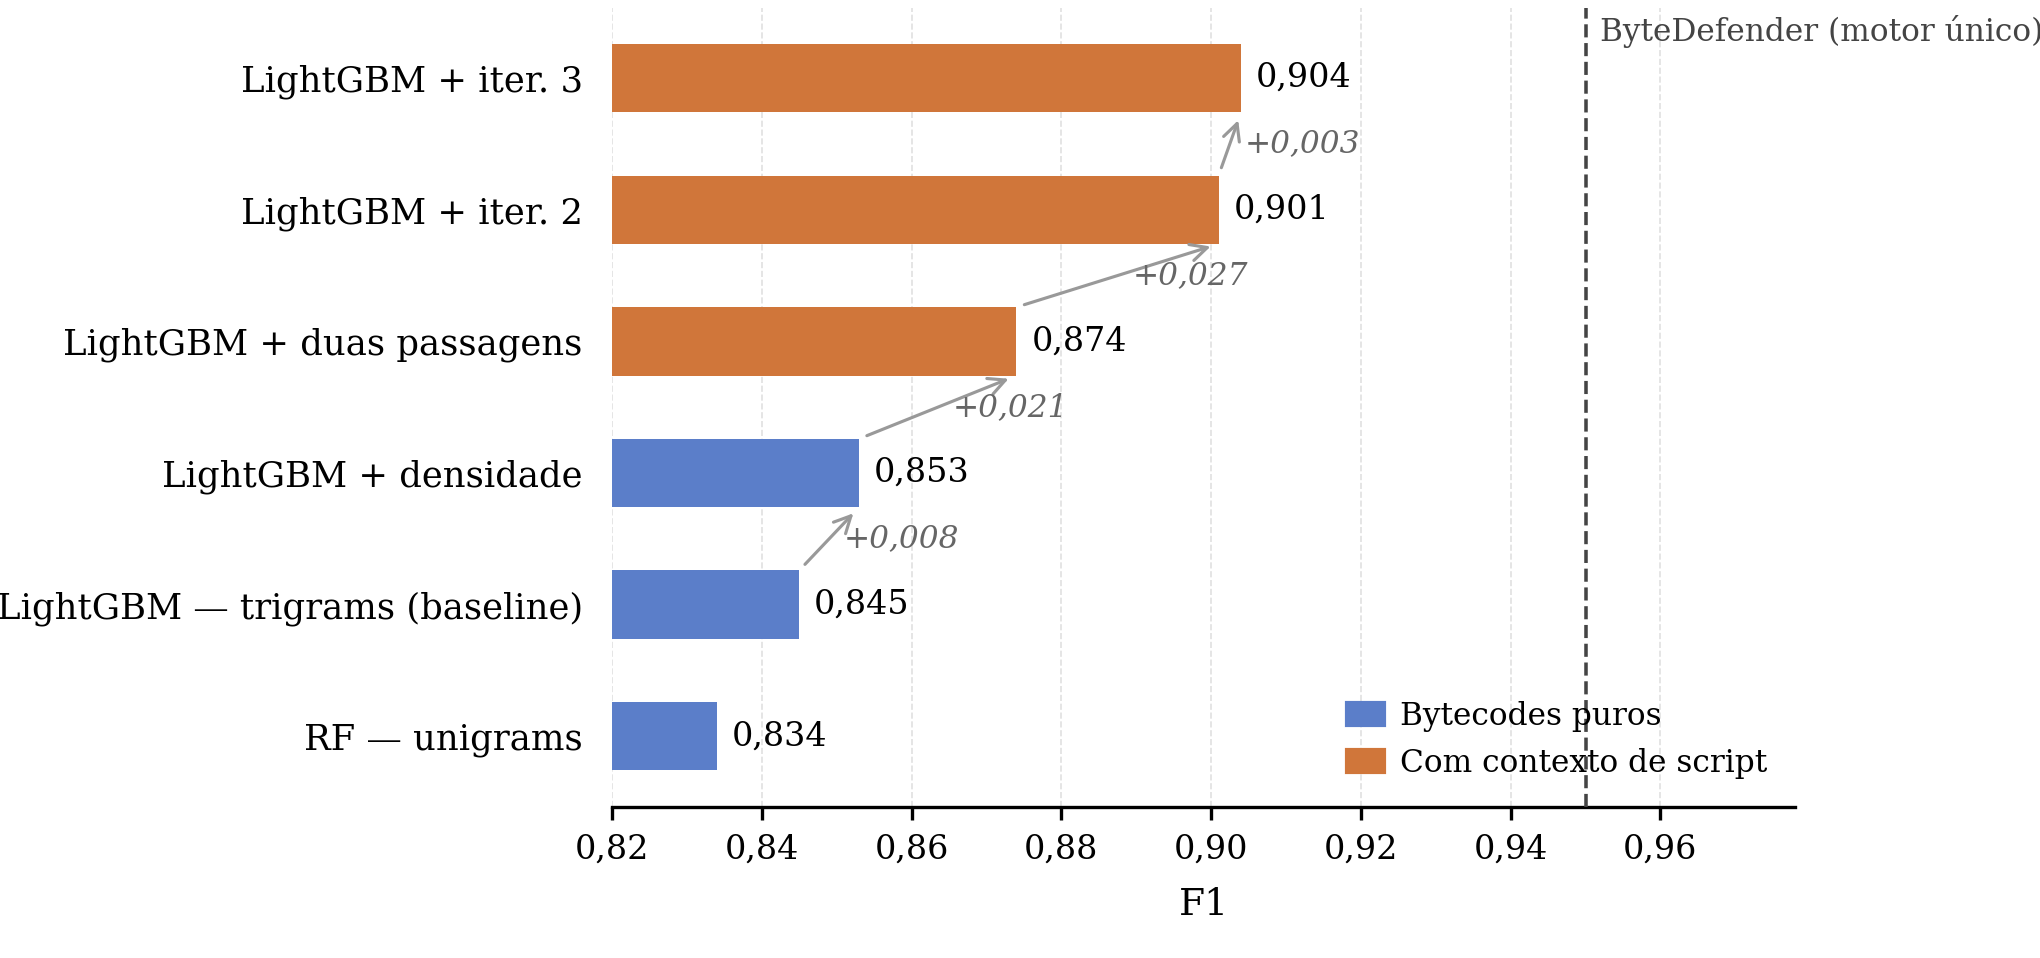
\includegraphics[width=0.88\linewidth]{fig_f1_progression}
\fonte{Elaborada pelo autor.}
\end{figure}

\textbf{RF como piso interpretativo.} O RF com unigrams (136~features) atinge
F1~=~0,834, confirmando que as frequências de tokens individuais da RI já codificam
sinal discriminativo substancial. Funções de fingerprinting são
caracterizadas por alta frequência de tokens de acesso a propriedades
(\texttt{get\_keyed\_prop}, \texttt{get\_named\_prop}) e de chamadas de método
(\texttt{call\_func}); esses padrões são suficientemente distintos para separar a
maioria dos positivos com um modelo simples de 136~features. Qualquer modelo mais
complexo deve superar esse piso para justificar a complexidade adicional.

\textbf{LightGBM com trigrams confirma o teto de n-gramas.} O LightGBM com trigrams
TF-IDF atinge F1~=~0,845 (P~=~0,885, R~=~0,809, limiar~=~0,80), ganho de apenas +0,002
sobre os bigrams apesar de 10,7$\times$ mais features (50.631 vs.\ 4.723). Esse plateau
indica que o espaço de n-gramas sobre 145 tokens está essencialmente exaurido nos bigrams;
os enriquecimentos de features subsequentes partem do modelo de bigrams (F1~=~0,843) como
referência, buscando superar o teto de bytecodes puros de $\approx$F1~0,85. A análise
detalhada está na Seção~\ref{sec:adicionais}.

%, , , , , , , , , , , , , , , , , , , --
\section{Contexto de script e inferência iterativa}
\label{sec:iterativo}

A principal limitação do LightGBM baseline é a classificação em isolamento: cada
função é avaliada independentemente, sem informação sobre o script em que está
inserida. Funções de fingerprinting tendem a co-ocorrer no mesmo script, uma biblioteca como \texttt{fingerprintjs} empacota dezenas de funções
especializadas em um único arquivo, e bibliotecas menores de WebGL ou áudio
raramente aparecem em scripts de propósito geral. Incorporar essa co-ocorrência sem
usar rótulos externos é o objetivo das três etapas desta seção.

\textbf{Densidade de script.} O primeiro estágio adiciona como feature a densidade
média de fingerprinting do script: a fração de funções no mesmo arquivo com
probabilidade prevista acima de 0,5, calculada com o LightGBM baseline em uma
passagem prévia sobre o dataset completo. Nenhum rótulo real é consultado. O
resultado é F1~=~0,853 (+0,008 sobre o baseline de trigrams, +0,019 sobre o RF,
P~=~0,883, R~=~0,825, limiar~=~0,80). O ganho de divisão dessa única feature (2.949)
é o maior de qualquer feature individual do modelo com densidade, superando qualquer bigram
TF-IDF \emph{nesse mesmo modelo}, e confirma que a co-ocorrência de script é um sinal genuinamente
informativo, irredutível à frequência de tokens por função. Nota: os ganhos de divisão
reportados aqui (escala de unidades a milhar) não são diretamente comparáveis com
os da Tabela~\ref{tab:features-imp}, que correspondem ao modelo de bigrams sem feature
de densidade; ao adicionar a densidade, o modelo redistribui parte substancial do
ganho para essa nova feature, reduzindo os ganhos individuais dos bigrams. Destaca-se ainda que
esse modelo usa apenas bigrams TF-IDF mais a feature de densidade (4.724 features
no total, cf.\ Tabela~\ref{tab:bin}), mas supera o baseline de trigrams
(50.631~features), demonstrando que uma feature de contexto de script vale mais do
que 10$\times$ mais n-grams.

\textbf{Inferência em duas passagens.} O segundo estágio enriquece o vetor de
contexto: além da densidade, acrescenta a contagem absoluta de funções com
probabilidade prevista acima de~0,5 e o logaritmo do tamanho total do script.
A motivação é que a densidade relativa e a contagem absoluta capturam aspectos
complementares: um script com 3 de 5 funções previstas como FP
(densidade~=~0,60) transmite sinal distinto de um com 3 de 300
(densidade~=~0,01), mesmo que a contagem absoluta seja idêntica. O resultado é
F1~=~0,874 (+0,021 sobre a densidade, P~=~0,901, R~=~0,848, limiar~=~0,80).

\textbf{Inferência iterativa com contagens em múltiplos limiares.} O terceiro
estágio substitui a contagem única por três contagens em limiares distintos
($p{>}0{,}30$; $p{>}0{,}50$; $p{>}0{,}70$), capturando a forma da
distribuição de probabilidades dentro de cada script. Um script com muitas funções
classificadas a $p \approx 0{,}4$ (positivos suaves) é qualitativamente diferente
de um com poucas funções a $p{>}0{,}70$ (positivos de alta confiança), mesmo que a
densidade seja semelhante. Com \texttt{neg\_ratio} = 7 e 1.000 árvores, a iteração~2 atinge
\textbf{F1~=~0,901} (P~=~0,917, R~=~0,886, limiar~=~0,70). Os split gains das features de contexto dominam todas as demais: 4.952
(densidade), 4.410 (logaritmo do tamanho), 4.149 (contagem $p{>}0{,}30$),
3.944 (contagem $p{>}0{,}70$), 3.391 (contagem $p{>}0{,}50$).

Um ciclo adicional de auto-melhora, recomputando as contagens com o modelo da
iteração~2 e retreinando com os mesmos parâmetros, produz
\textbf{F1~=~0,904} (P~=~0,934, R~=~0,876, limiar~=~0,80, iter.~3). A progressão
por iteração é +0,021, +0,027, +0,003, confirmando convergência gradual com
retornos decrescentes a partir da iteração~2. O modelo da iteração~3 é o
\textbf{resultado implantável principal deste trabalho}: F1~=~0,904 sem nenhum
rótulo prévio, usando apenas predições do próprio modelo iteradas sobre o corpus
completo.

%, , , , , , , , , , , , , , , , , , , --
\section{Generalização cross-engine}
\label{sec:crossengine}

\subsection{Transferência zero-shot}
\label{sub:zeroshot}

O experimento de transferência zero-shot treina o LightGBM de bigrams sobre
funções de um único motor (conjunto completo de dados disponível para esse motor) e
avalia sobre o conjunto completo do outro motor. Nenhum dado do motor de teste está
disponível durante o treinamento.

\begin{table}[htb]
\centering
\caption{Transferência zero-shot (LightGBM bigrams, sem dados do motor de teste)}
\label{tab:zeroshot}
{\small
\begin{tabular}{lrrrrrrl}
\toprule
\textbf{Treino $\to$ Teste} & \textbf{Tam.\ treino} & \textbf{Tam.\ teste} & \textbf{FP teste} & \textbf{Limiar} & \textbf{P} & \textbf{R} & \textbf{F1} \\
\midrule
Chromium $\to$ Firefox & 191.565 & 296.610 & 27.312 & 0,05 & 0,093 & 0,363 & \textbf{0,149} \\
Firefox $\to$ Chromium & 296.965 & 191.692 & 14.047 & 0,05 & 0,123 & 0,341 & \textbf{0,180} \\
\bottomrule
\end{tabular}
}% end \small
{\footnotesize As leves diferenças entre o tamanho de treino e de teste de um mesmo
motor (ex.: Firefox treino 296.965 vs.\ teste 296.610) decorrem da estratificação
por \texttt{is\_fp} realizada independentemente em cada direção do experimento.}

\fonte{Elaborada pelo autor.}
\end{table}

Os limiares de 0,05 revelam o estado de colapso do classificador: para obter
qualquer revocação razoável, é necessário aceitar um número massivo de falsos
positivos. A precisão de 0,093--0,123 corresponde a aproximadamente 1 verdadeiro
positivo para cada 7--10 alarmes falsos. O F1 de 0,149--0,180 confirma que a
transferência zero-shot falha completamente.

A causa é estrutural: TF-IDF sobre bigrams captura padrões de sequência locais.
Embora ambos os motores compartilhem o mesmo vocabulário de tokens de RI após a
tradução, as distribuições de n-grams diferem sistematicamente: V8 e
SpiderMonkey compilam a mesma operação JavaScript em ordens de tokens distintas
(ver Seção~\ref{sec:ir-motivacao}). O modelo aprende limites de decisão moldados
pela distribuição de bigrams do motor de origem; esses limites não se transferem.

\subsection{Modelo conjunto por motor}
\label{sub:conjunto}

O experimento de modelo conjunto treina um único LightGBM de bigrams sobre a
amostra mista (dados de ambos os motores), usando a divisão cross-engine 80/20
estratificada descrita na Tabela~\ref{tab:split-exp} (33.087~FP treino, 8.272~FP
teste — totais maiores que os 37.644 da divisão padrão por incluir registros
independentes de cada motor). O conjunto de teste é então filtrado por
motor para avaliar o desempenho por engine separadamente, sem vazamento de dados de
treinamento.

\begin{table}[htb]
\centering
\caption{Modelo conjunto bigrams: avaliação por motor no conjunto de teste (LightGBM bigrams)}
\label{tab:conjunto}
\begin{tabular}{lrrrr}
\toprule
\textbf{Motor} & \textbf{P} & \textbf{R} & \textbf{F1} & \textbf{Suporte FP} \\
\midrule
Chromium (V8)            & 0,933 & 0,828 & \textbf{0,877} & 2.873 \\
Firefox (SpiderMonkey)   & 0,864 & 0,830 & \textbf{0,847} & 5.399 \\
\midrule
\textbf{Média ponderada} & 0,888 & 0,829 & \textbf{0,857} & 8.272 \\
\bottomrule
\end{tabular}

\fonte{Elaborada pelo autor.}
\end{table}

A média ponderada de 0,857 coincide exatamente com o F1 global do modelo
(Tabela~\ref{tab:conjunto}), confirmando que a divisão de teste está balanceada entre os
motores e que a avaliação é internamente consistente, não há viés de amostragem
que favorecesse um motor no conjunto de teste global.

O modelo conjunto atinge F1~=~0,877 no Chromium e F1~=~0,847 no Firefox a partir
de um único conjunto de pesos, sem retreinamento por motor. O F1 global de 0,857
corresponde à média ponderada pelo suporte desses dois valores (Tabela~\ref{tab:conjunto}),
confirmando consistência entre a avaliação por motor e a métrica global.
A diferença de $\approx$0,030 entre os motores (0,877 vs.\ 0,847) é consistente com
a maior regularidade estrutural dos bytecodes do V8 (máquina de registradores, sequências
mais compactas) em relação ao SpiderMonkey (máquina de pilha, maior verbosidade), que
produz padrões de n-gramas V8 mais uniformes e portanto mais discriminativos para o
classificador TF-IDF.

Quando o modelo conjunto é aumentado com as mesmas cinco features de contexto
iterativo da Tabela~\ref{tab:bin} (densidade de script, três contagens por limiar e
tamanho), o desempenho por motor melhora significativamente.

\begin{table}[htb]
\centering
\caption{Modelo conjunto com contexto iterativo (iter~3): avaliação por motor}
\label{tab:conjunto-iter}
{\footnotesize
Avaliado na divisão padrão (Tabela~\ref{tab:split}: 7.529~FP de teste total,
1.521 Chromium + 6.008 Firefox), diferente da divisão cross-engine usada na
Tabela~\ref{tab:conjunto} (8.272~FP). Os suportes por motor diferem entre as
duas tabelas porque os datasets foram construídos com estratégias de amostragem
distintas: a divisão padrão parte do dataset unificado (37.644~FP, razão
Firefox:Chromium de $\approx$4:1 no corpus), enquanto a divisão cross-engine
amostra cada motor independentemente, elevando o total de FP (41.359) e
redistribuindo a proporção relativa entre os motores. A comparação direta
de F1 entre as tabelas é, portanto, aproximada.
}

\bigskip
\begin{tabular}{lrrrr}
\toprule
\textbf{Motor} & \textbf{P} & \textbf{R} & \textbf{F1} & \textbf{Suporte FP} \\
\midrule
Chromium (V8)            & 0,941 & 0,869 & \textbf{0,903} & 1.521 \\
Firefox (SpiderMonkey)   & 0,932 & 0,878 & \textbf{0,904} & 6.008 \\
\bottomrule
\end{tabular}

\fonte{Elaborada pelo autor.}
\end{table}

O modelo iterativo atinge F1~=~0,903 no Chromium e F1~=~0,904
no Firefox (divisão padrão). A homogeneidade entre motores, diferença de apenas 0,001, confirma
que a RI com treinamento conjunto produz representações igualmente úteis para ambos
os engines quando complementadas por contexto de script.

%, , , , , , , , , , , , , , , , , , , --
\section{Importância de features}
\label{sec:features}

A Tabela~\ref{tab:features-imp} apresenta as 15 features de maior ganho de divisão
(split gain) no modelo LightGBM de bigrams. O ganho de divisão mede a
redução total de impureza atribuída a cada feature ao longo de todas as árvores e
divisões do ensemble.

\begin{table}[htb]
\centering
\caption{Top-15 features por ganho de divisão (LightGBM bigrams)}
\label{tab:features-imp}
\begin{tabular}{rlrr}
\toprule
\textbf{Rank} & \textbf{Feature (token ou bigram de RI)} & \textbf{Ganho} & \textbf{Divisões} \\
\midrule
 1 & \texttt{get\_keyed\_prop}                  & 718.016 &  280 \\
 2 & \texttt{load\_closure\_var}                & 249.551 &  787 \\
 3 & \texttt{call\_func get\_keyed\_prop}        & 237.632 &  163 \\
 4 & \texttt{get\_named\_prop}                  & 211.451 &  700 \\
 5 & \texttt{return}                            & 195.687 &  961 \\
 6 & \texttt{call\_func}                        & 166.258 &  669 \\
 7 & \texttt{load\_closure\_var call\_func}     &  83.605 &  241 \\
 8 & \texttt{load\_undefined call\_func}        &  83.188 &  243 \\
 9 & \texttt{pop\_scope}                        &  81.646 &  125 \\
10 & \texttt{call\_func pop}                    &  80.206 &  390 \\
11 & \texttt{store\_closure\_var}               &  79.208 &  356 \\
12 & \texttt{load\_undefined set\_exception}    &  69.639 &   51 \\
13 & \texttt{call\_func store\_local}           &  62.009 &  358 \\
14 & \texttt{load\_global get\_named\_prop}     &  61.085 &  170 \\
15 & \texttt{call\_func return}                 &  59.609 &  351 \\
\bottomrule
\end{tabular}

\fonte{Elaborada pelo autor.}
\end{table}

\textbf{\texttt{get\_keyed\_prop}} lidera com folga (ganho 718.016, quase 3$\times$
o segundo colocado), refletindo o padrão central de fingerprinting: acessar
propriedades indexadas de objetos de API como \texttt{gl.getParameter(pname)} ou
\texttt{screen[prop]}. Esse padrão está presente em todas as sete categorias de
fingerprinting.

\textbf{\texttt{load\_closure\_var}} (ganho 249.551, 787 divisões, o segundo maior
número de divisões na lista, abaixo apenas de \texttt{return} com 961) codifica o uso de closures típico de
bibliotecas de fingerprinting empacotadas em IIFE (Immediately Invoked
Function Expressions): os resultados intermediários são armazenados e recuperados
via variáveis de closure entre funções internas do módulo.

\textbf{Bigrams de acesso-chamada} como \texttt{call\_func get\_keyed\_prop} e
\texttt{load\_closure\_var call\_func} capturam a sequência invoke-then-read:
chamar um método de API e imediatamente ler a propriedade do resultado, padrão
idiomático em WebGL (\texttt{gl.getParameter(...)}) e Canvas
(\texttt{ctx.measureText(...).width}).

\textbf{\texttt{load\_undefined set\_exception}} (rank~12, 51 divisões, alto ganho
por divisão: $\approx$1.366 por divisão) corresponde ao bloco
\texttt{try \{ ... \} catch(e) \{\}} que bibliotecas de fingerprinting usam
para testar a disponibilidade de APIs de forma resiliente entre navegadores. Esse
padrão é altamente discriminativo por seu ganho por divisão elevado, cada vez
que o modelo usa essa feature, ela reduz substancialmente a impureza do nó.

A predominância de tokens de acesso a propriedades (\texttt{get\_keyed\_prop},
\texttt{get\_named\_prop}, \texttt{load\_global get\_named\_prop}) e de chamadas
de função/método (\texttt{call\_func}, \texttt{call\_func get\_keyed\_prop}) na
lista reflete a natureza de fingerprinting: coleta sistemática de
propriedades de objetos de API do browser, encadeada com chamadas que processam ou
armazenam os resultados.

%, , , , , , , , , , , , , , , , , , , --
\section{Experimentos Adicionais}
\label{sec:adicionais}

Esta seção consolida experimentos que complementam a linha principal com contexto
comparativo sobre outras famílias de modelos, variantes de features e o limite
superior oracle.

\subsection{Expansão para trigrams e teto de bytecodes}
\label{sub:trigrams}

Bigrams e trigrams TF-IDF atingem respectivamente F1~=~0,843 e F1~=~0,845
(4.723 vs.\ 50.631 features). O gap entre bigrams e
trigrams (teto de bytecodes puros em $\approx$F1~0,85)
não se fecha ao se acrescentar mais features, e bigrams+densidade supera o baseline
de trigrams com apenas 4.724~features, confirmando a interpretação. O plateau entre bigrams e trigrams é
explicado na Seção~\ref{sec:disc-teto}: os trigrams reexpressam combinações de
bigrams discriminativos sem introduzir informação nova, pois o comportamento de
fingerprinting se concentra em poucos padrões de opcode que já estão cobertos
pelos bigrams retidos.

\subsection{SVM}
\label{sub:svm-exp}

O SVM com gradiente estocástico e perda de dobradiça, calibrado em
probabilidades, sobre TF-IDF de bigrams, atinge F1~=~0,649 (P~=~0,644,
R~=~0,653, limiar~=~0,35), bem abaixo do LightGBM com as mesmas features
(F1~=~0,843) e abaixo até do RF com unigrams (F1~=~0,834). A calibração de
probabilidades introduz ruído nos limiares de decisão, e o gradiente estocástico
com perda de dobradiça produz margens menos estáveis do que o LightGBM com
histogram splitting no regime de alta dimensionalidade esparsa.

\subsection{BiLSTM}
\label{sub:bilstm}

Uma BiLSTM de duas camadas (256 unidades ocultas, embedding $145 \times 64$
RI com separação de aridade descrita na Seção~\ref{sub:aridade},
pooling mean+max) treinada atinge F1~=~0,856 (P~=~0,894,
R~=~0,821, limiar~=~0,95), superior em +0,013~F1 ao LightGBM de bigrams
(F1~=~0,843), mas com modelo substancialmente mais pesado e maior custo de
treinamento. O ganho marginal confirma que a informação sequencial captada pelo BiLSTM
não acrescenta discriminação substancial além do que o TF-IDF de bigrams já codifica;
o vocabulário fechado de 145~tokens limita a vantagem de qualquer representação sequencial.

\subsection{Transformer}
\label{sub:transformer}

\textbf{Versão~1 (FastText fixo, F1~=~0,415):} O Transformer original (2 camadas
de codificador, embeddings FastText 128-dim fixos, Focal Loss, treinado
em 4$\times$ Tesla P100-SXM2) obteve resultado anomalamente baixo. A investigação
identificou três causas: (1)~bug de conversão de tipo nas sequências de entrada;
(2)~Focal Loss instável com vocabulário fechado de 145~tokens; (3)~embeddings
fixos que impedem adaptação ao domínio.

\textbf{Versão~2 (embeddings treináveis, F1~=~0,764):} Corrigidos os três
problemas --- conversão correta de tipos nas entradas, substituição da Focal
Loss por BCE ponderada e embeddings iniciados aleatoriamente e treinados
conjuntamente --- com pooling mean+max em vez de mean-only, o modelo atinge
F1~=~0,764 (P~=~0,817, R~=~0,717, limiar~=~0,85). O gap remanescente em
relação ao LightGBM ($\approx$0,09~F1) reflete uma limitação arquitetural: com
sequências de tokens altamente repetidos (ex.: 50$\times$ \texttt{load\_local} em
uma mesma função), o mecanismo de auto-atenção degenera em bag-of-words,
perdendo a vantagem posicional que o Transformer deveria oferecer.

\subsection{Features estruturais locais}
\label{sub:estrutural}

Seis features escalares derivadas da sequência de tokens de RI — contagem de tokens,
contagem de leituras de propriedades, contagem de chamadas, densidade de leituras
de propriedades, número de tipos distintos e presença de variável de fechamento —
foram acrescentadas ao LightGBM de bigrams. O resultado é F1~=~0,842
(P~=~0,886, R~=~0,801, 4.729 features): ganho nulo ($\approx{-}0{,}001$) em relação
ao baseline de bigrams (F1~=~0,843).
As features estruturais não carregam informação independente porque as frequências
TF-IDF já as codificam implicitamente: uma função densa em tokens \texttt{call\_*}
terá alta frequência nesses unigrams, e o TF-IDF já captura isso como feature
individual.

\subsection{IR com separação de aridade}
\label{sub:aridade}

O dicionário base (Apêndice~\ref{ap:ir-dict}) mantém separação de aridade para
opcodes V8 de chamada de função (\texttt{CALL\_FUNC\_0}, \texttt{CALL\_FUNC\_1},
\texttt{CALL\_FUNC\_2}, \texttt{CALL\_FUNC\_N}, \texttt{CALL\_METHOD\_0},
\texttt{CALL\_METHOD\_1}, \texttt{CALL\_METHOD\_2}, \texttt{CALL\_METHOD\_N}),
refletindo que o V8 emite opcodes distintos conforme o número de argumentos
(\texttt{CallUndefinedReceiver0}, \texttt{CallUndefinedReceiver1}, etc.). Uma
variante experimental colapsa esses oito tokens em dois (\texttt{CALL\_FUNC} e
\texttt{CALL\_METHOD\_N}), na hipótese de que a granularidade de aridade não
acrescentaria discriminação útil. O LightGBM com bigrams sobre essa variante
colapsada (4.623~features) atinge F1~=~0,857, equivalente ao modelo base de bigrams
(4.723~features). A redução no número de features da variante colapsada (4.623 vs.\ 4.723~do modelo base)
é atenuada pelo aumento de frequência dos tokens fundidos, que fazem mais bigramas
superarem o limiar mínimo de frequência (\texttt{min\_df}).
A aridade das chamadas não acrescenta informação discriminativa sobre o tipo de função.

\subsection{Classificadores multilabel}
\label{sec:multilabel}

A Tabela~\ref{tab:multilabel} apresenta os resultados por categoria e o macro-F1
para os três modelos multilabel. O suporte de teste por rótulo reflete a
distribuição apresentada no Capítulo~\ref{cap:dataset}.

\begin{table}[htb]
\centering
\caption{Classificadores multilabel: 7 categorias de fingerprinting}
\label{tab:multilabel}
{\footnotesize
Mesma divisão e features da Tabela~\ref{tab:bin}. Suporte de teste: Canvas~1.635,
Áudio~182, WebRTC~39, Fonte~39, WebGL~2.001, Tela~5.323, Navigator~2.844.
}

\bigskip
\resizebox{\linewidth}{!}{%
\begin{tabular}{lrrrrrrrl}
\toprule
\textbf{Modelo} & \textbf{Canvas} & \textbf{Áudio} & \textbf{WebRTC} & \textbf{Fonte} & \textbf{WebGL} & \textbf{Tela} & \textbf{Navigator} & \textbf{Macro-F1} \\
\midrule
RF (200 árvores, bal.\ por subamostragem) & 0,687 & 0,480 & 0,201 & 0,345 & 0,729 & 0,755 & 0,747 & \textbf{0,564} \\
LightGBM (classificador multirrótulo)      & 0,818 & 0,198 & 0,001 & 0,001 & 0,826 & 0,758 & 0,788 & 0,484 \\
Transformer (Focal Loss)                & 0,204 & 0,075 & 0,017 & 0,013 & 0,288 & 0,279 & 0,320 & 0,171 \\
\bottomrule
\end{tabular}%
}
\fonte{Elaborada pelo autor.}
\end{table}

\textbf{O RF é o melhor modelo multilabel} (macro-F1~=~0,564). A estratégia de
balanceamento por subamostragem por árvore reamostra cada árvore
individualmente, produzindo classificadores por rótulo mais robustos a
desequilíbrios extremos do que a abordagem de pesos globais do LightGBM. O
LightGBM com balanceamento automático de classes colapsa nos rótulos raros: o
classificador WebRTC atinge P~=~0,0007 (F1~=~0,001), predizendo positivo para
quase todas as funções do conjunto de teste. O Transformer com Focal Loss não converge para
representações úteis nos rótulos raros com apenas 39 positivos de teste para os rótulos raros
(WebRTC e Fonte; suporte do conjunto de teste, ver nota da tabela). Para
os rótulos bem suportados (Tela, WebGL, Navigator, Canvas), todos os três modelos
produzem F1 acima de~0,68, confirmando que os bytecodes da RI carregam sinal
multilabel genuíno quando o suporte é adequado. A discussão completa está na
Seção~\ref{sec:disc-raro}.

\subsection{Benchmark de inferência}
\label{sec:inferencia}

\begin{table}[htb]
\centering
\caption{Benchmark de inferência: LightGBM bigrams (CPU, processo único)}
\label{tab:inferencia}
{\footnotesize
$n_{\text{reps}}$: número de repetições para estimativa de média e percentis.
Medições em ambiente quiescente; p99 inclui variação de sistema operacional.
}

\bigskip
{\small
\begin{tabular}{rrrrrrl}
\toprule
\textbf{Lote} & \textbf{$n_{\text{reps}}$} & \textbf{Média (ms)} & \textbf{p50 (ms)} & \textbf{p95 (ms)} & \textbf{p99 (ms)} & \textbf{Por função (µs)} \\
\midrule
    1 & 200 &  3,31 &  2,84 &  4,08 & 18,73 & 3.308 \\
   10 &  20 &  4,19 &  3,31 &  5,74 & 16,23 &   419 \\
  100 &   5 &  9,28 &  8,95 &  9,91 &  9,98 &  92,8 \\
1.000 &   5 & 44,15 & 44,05 & 45,64 & 45,87 & \textbf{44,1} \\
\bottomrule
\end{tabular}
}% end \small
\fonte{Elaborada pelo autor.}
\end{table}

Com lote de 1.000 funções, o modelo classifica a \textbf{44,1~µs por função}
(vazão de $\approx$22.700~funções/segundo). O traço de bytecodes de uma página web
típica, algumas centenas de funções JavaScript, seria classificado em menos
de 15~ms. Com lote unitário, a latência de 3,31~ms é dominada pela construção da
matriz TF-IDF esparsa; em produção, o processamento em lote elimina esse custo
fixo. A discussão de cenários de implantação está na
Seção~\ref{sec:disc-implantacao}.

\subsection{Limite superior oracle}
\label{sec:oracle}

O modelo oracle (LightGBM + bigrams + densidade de script + 6~features estruturais
+ 4~features de contexto de script real) atinge \textbf{F1~=~0,928} (P~=~0,944, R~=~0,912,
limiar~=~0,90). As features de contexto real são: contagem absoluta de funções FP
no mesmo script, contagem total de funções, razão entre elas e logaritmo do
tamanho, calculadas sobre as 68M linhas do dataset antes da divisão
treino/teste, com os rótulos reais.

\textbf{Este resultado não é implantável.} Em produção, os rótulos reais não estão
disponíveis no momento da classificação. O modelo oracle estabelece um
limite superior para sistemas de co-ocorrência de script: o desempenho
atingível se todas as funções vizinhas de um script fossem previamente rotuladas
com perfeição. O modelo iterativo (iter.~3, F1~=~0,904) recupera $\approx$68\%
desse intervalo sem consultar nenhum rótulo real; a diferença remanescente de 0,024
e sua irredutibilidade são analisadas na Seção~\ref{sec:disc-teto}.

% ============================================================
%  Capítulo 7 — Discussão
% ============================================================
\chapter{DISCUSSÃO}
\label{cap:discussao}

\section{Teto de informação da representação intermediária}
\label{sec:disc-teto}

O resultado mais revelador da Tabela~\ref{tab:bin} não é o melhor F1 absoluto, mas
a resposta quase nula à expansão do espaço de features: passar de bigrams
(4.723~features, F1~=~0,843) para trigrams (50.631~features, F1~=~0,845) representa
um ganho de apenas +0,002 apesar de uma expansão 10,7$\times$ no número de
features. Essa resposta plana indica um teto imposto pela entrada, não pela
capacidade do modelo.

A aritmética do vocabulário explica o fenômeno. O vocabulário da RI contém 136
tokens ativos. Como os bigrams TF-IDF são ordenados (o par
\texttt{load\_global get\_named\_prop} é distinto de
\texttt{get\_named\_prop load\_arg}), o número máximo de bigrams distintos é
$136^2 = 18.496$; o máximo de trigrams é da ordem de
$136^3 \approx 2{,}5 \times 10^6$. O TF-IDF retém, respectivamente, 4.723 e
50.631 features por frequência mínima, ou seja, apenas os n-grams que aparecem
com frequência suficiente no corpus de treinamento. Como o comportamento de
fingerprinting se concentra num subconjunto pequeno de padrões de opcode
(acesso a propriedades, captura de closure, chamadas de API,
try/catch), os bigrams discriminativos estão praticamente exauridos dentro
das 4.723 features retidas. Trigrams adicionam cadeias mais longas, mas estas
apenas reexpressam padrões já capturados por combinações de bigrams; não introduzem
informação nova.

O RF com unigrams (136~features, F1~=~0,834) reforça essa conclusão por outro
ângulo: a frequência de tokens individuais, sem qualquer noção de ordem ou
co-ocorrência, já alcança 0,011 abaixo do melhor modelo. A contribuição marginal de
cada nível de n-gram é decrescente e pequena.

O teto situa-se em aproximadamente \textbf{F1 $\approx$ 0,85} para detecção
cross-engine baseada exclusivamente em bytecodes. Os $\approx$15\% de erro residual
não podem ser fechados com n-grams mais ricos sobre o mesmo vocabulário de 145
tokens. Três fontes de informação ausentes nos bytecodes poderiam reduzir esse
erro:

\begin{enumerate}
\item \textbf{Nomes de funções e contexto de grafo de chamadas.} O modelo atual não
  distingue uma função \texttt{canvasFingerprint} de uma função
  \texttt{renderButton} se ambas produzirem sequências de RI similares. Nomes e
  posição no grafo de chamadas identificam funções orquestradoras que não tocam a
  API diretamente.

\item \textbf{Valores em tempo de execução.} Um mesmo bytecode
  \texttt{GET\_NAMED\_PROP} pode ler \texttt{screen.width} (FP) ou
  \texttt{div.offsetWidth} (layout legítimo). A distinção requer conhecimento do
  valor do receptor, informação ausente no traço estático de bytecodes.

\item \textbf{Vocabulário de opcodes mais fino.} A RI abstrai variantes de opcodes
  que o V8 e o SpiderMonkey distinguem (ex.: \texttt{LdaSmi} vs.\
  \texttt{LdaConstant} $\to$ ambos \texttt{LOAD\_INT}). Preservar essas distinções
  aumentaria a expressividade, ao custo de reduzir a portabilidade entre motores.
\end{enumerate}

\textbf{Features estruturais e contexto de script.} Para testar se o teto poderia
ser elevado sem abandonar a resistência à ofuscação, dois grupos de features
adicionais foram avaliados via ablação (Seções~\ref{sub:estrutural}
e~\ref{sec:oracle}). O primeiro, seis features estruturais locais derivadas
diretamente da sequência de tokens da RI, não produziu ganho mensurável sobre
o baseline de bigrams (F1~=~0,842~vs.~0,843, $\approx{-}0{,}001$), confirmando que as frequências
TF-IDF já codificam implicitamente essas estatísticas. O segundo grupo, contagem
real de funções FP no mesmo script, calculada sobre as 68M linhas com os rótulos
reais do dataset, produziu um salto de +0,075~F1 (F1~=~0,928
vs.~0,853). Esse experimento delimita o \textbf{limite superior oracle}:
o desempenho máximo atingível pela co-ocorrência de script, pressupondo perfeita
rotulagem prévia de todas as funções vizinhas. Como essa condição não se verifica
em produção, F1~=~0,928 não é implantável (ver Seção~\ref{sec:oracle}).

\textbf{Inferência iterativa: F1~=~0,904 sem rótulos oracle.} Para recuperar parte
do intervalo de 0,075 sem vazar rótulos, foi implementada uma estratégia de
inferência iterativa. A primeira passagem classifica todas as 68M funções com o
modelo de densidade e acumula, por script, a contagem absoluta de funções com
probabilidade acima de 0,50 e o logaritmo do tamanho total.
Nenhum rótulo real é consultado. A segunda passagem retreina o LightGBM com essas
três features de contexto (densidade, contagem e logaritmo do tamanho), atingindo
F1~=~0,874. Ciclos adicionais de auto-melhora, expandindo para três contagens em
limiares distintos ($p{>}0{,}30$; $p{>}0{,}50$; $p{>}0{,}70$) e recomputando as
contagens com o modelo da iteração anterior, produzem \textbf{F1~=~0,901} (iter.~2)
e \textbf{F1~=~0,904} (P~=~0,934, R~=~0,876, limiar~=~0,80, iter.~3). A progressão
por iteração é +0,021, +0,027, +0,003, confirmando convergência com retornos
decrescentes. O modelo da
iteração~3 recupera $\approx$68\% do intervalo oracle (0,051 de 0,075) e é o
\textbf{resultado implantável principal} deste trabalho: F1~=~0,904 atingível
sem nenhum rótulo prévio.

A estratégia de contagens em múltiplos limiares captura a forma da
distribuição de probabilidades dentro de cada script: um script com muitas funções
a $p \approx 0{,}4$ (positivos suaves) é qualitativamente diferente de um com
poucas funções a $p{>}0{,}70$ (positivos de alta confiança), mesmo que o número de
funções com $p{>}0{,}5$ seja idêntico. Os split gains das cinco features de
contexto dominam as colunas de importância \emph{no modelo iterativo}, superando
individualmente os bigrams TF-IDF mais informativos nesse mesmo modelo. Nota: os
ganhos do modelo iterativo (escala de unidades a milhar, 1.000 árvores, com
features de contexto que redistribuem o ganho) não são diretamente comparáveis
com os da Tabela~\ref{tab:features-imp}, que apresenta os ganhos do modelo base
de bigrams sem contexto (500 árvores, escala de centenas de milhares).

\textbf{Irredutibilidade do intervalo remanescente.} Uma questão natural é se o
contexto de grafo de chamadas (identificar quais funções orquestradoras invocam
rotinas FP sem tocar a API diretamente) poderia fechar a diferença de 0,024
ainda existente. Para verificar isso empiricamente, os registros de chamadas de API produzidos
pelo script de conteúdo da extensão foram inspecionados. A extensão captura
pilhas de chamadas completas: registros consecutivos com o mesmo par
\texttt{(api, page\_url)} representam quadros sucessivos de uma única cadeia de
chamadas, do invocador direto da API até todos os envolvedores orquestradores.
Entretanto, o pós-processador já consome essa informação integralmente via
propagação de contenção: toda função que apareça em qualquer posição de uma
pilha de chamadas capturada é rotulada como FP, independentemente de ter invocado
a API diretamente. Os rótulos de cadeia de chamadas já estão presentes nos dados de
treinamento; nenhum sinal novo é extraível dos registros de pilha existentes.

A diferença remanescente de 0,024 não reflete ausência de cobertura do grafo de
chamadas. Ela reflete uma classe de sequências de bytecodes genuinamente ambíguas:
funções stub intermediárias corretamente rotuladas como FP por participarem da cadeia
de chamadas, mas cujas sequências de tokens de RI são indistinguíveis de
closures utilitárias comuns (comprimento médio $\approx$96~tokens — acima da
média do corpus de $\approx$65~tokens, pois são funções orquestradoras com
alguma lógica de controle —, fluxo de controle genérico, nenhuma assinatura de opcode específica de API). Nenhuma feature
derivável do dataset existente pode resolver essa ambiguidade. Fechá-la exigiria
informação que bytecodes estáticos não carregam: valores em tempo de execução que
distinguem \texttt{screen.width} de \texttt{div.offsetWidth}, ou nomes de fonte que
identificam \texttt{canvasFingerprint} em vez de \texttt{renderHelper}. Esse
resultado estabelece um teto superior principiado, no nível do dataset, que
profissionais podem usar para avaliar quando abordagens baseadas exclusivamente em
bytecodes são suficientes e quando sinais complementares precisam ser adicionados.

%, , , , , , , , , , , , , , , , , , , --
\section{Necessidade do treinamento conjunto}
\label{sec:disc-conjunto}

A existência de uma RI com vocabulário compartilhado é condição necessária,
mas não suficiente, para a generalização cross-engine. Os experimentos de
transferência zero-shot (Tabela~\ref{tab:zeroshot}) demonstram isso empiricamente:
mesmo com os mesmos 136 tokens de RI em ambos os motores, treinar em Chromium e
testar em Firefox produz F1~=~0,149; a direção inversa produz F1~=~0,180. Ambos os
resultados são próximos de um classificador aleatório calibrado para alta
revocação.

A causa é distribucional. V8 e SpiderMonkey compilam operações JavaScript
semanticamente idênticas em ordens de tokens distintas, como discutido na
Seção~\ref{sec:ir-motivacao}. Um bigram como \texttt{load\_global get\_named\_prop}
é frequente em sequências V8 para o padrão \texttt{navigator.hardwareConcurrency};
o SpiderMonkey pode produzir \texttt{get\_named\_prop load\_arg} para a mesma
operação. Após a tradução para RI, os unigrams são idênticos, mas os
bigrams diferem — a Figura~\ref{fig:zeroshot-vs-conjunto} ilustra essa
divergência nas distribuições de bigramas por motor. Um classificador TF-IDF
treinado exclusivamente em sequências V8 aprende limiares de decisão moldados
pela distribuição de bigrams do V8; esses limiares não transferem para a
distribuição estruturalmente diferente do SpiderMonkey.

\begin{figure}[htb]
\centering
\caption{Distribuições de bigramas de RI por motor: divergência entre V8 e SpiderMonkey}
\label{fig:zeroshot-vs-conjunto}
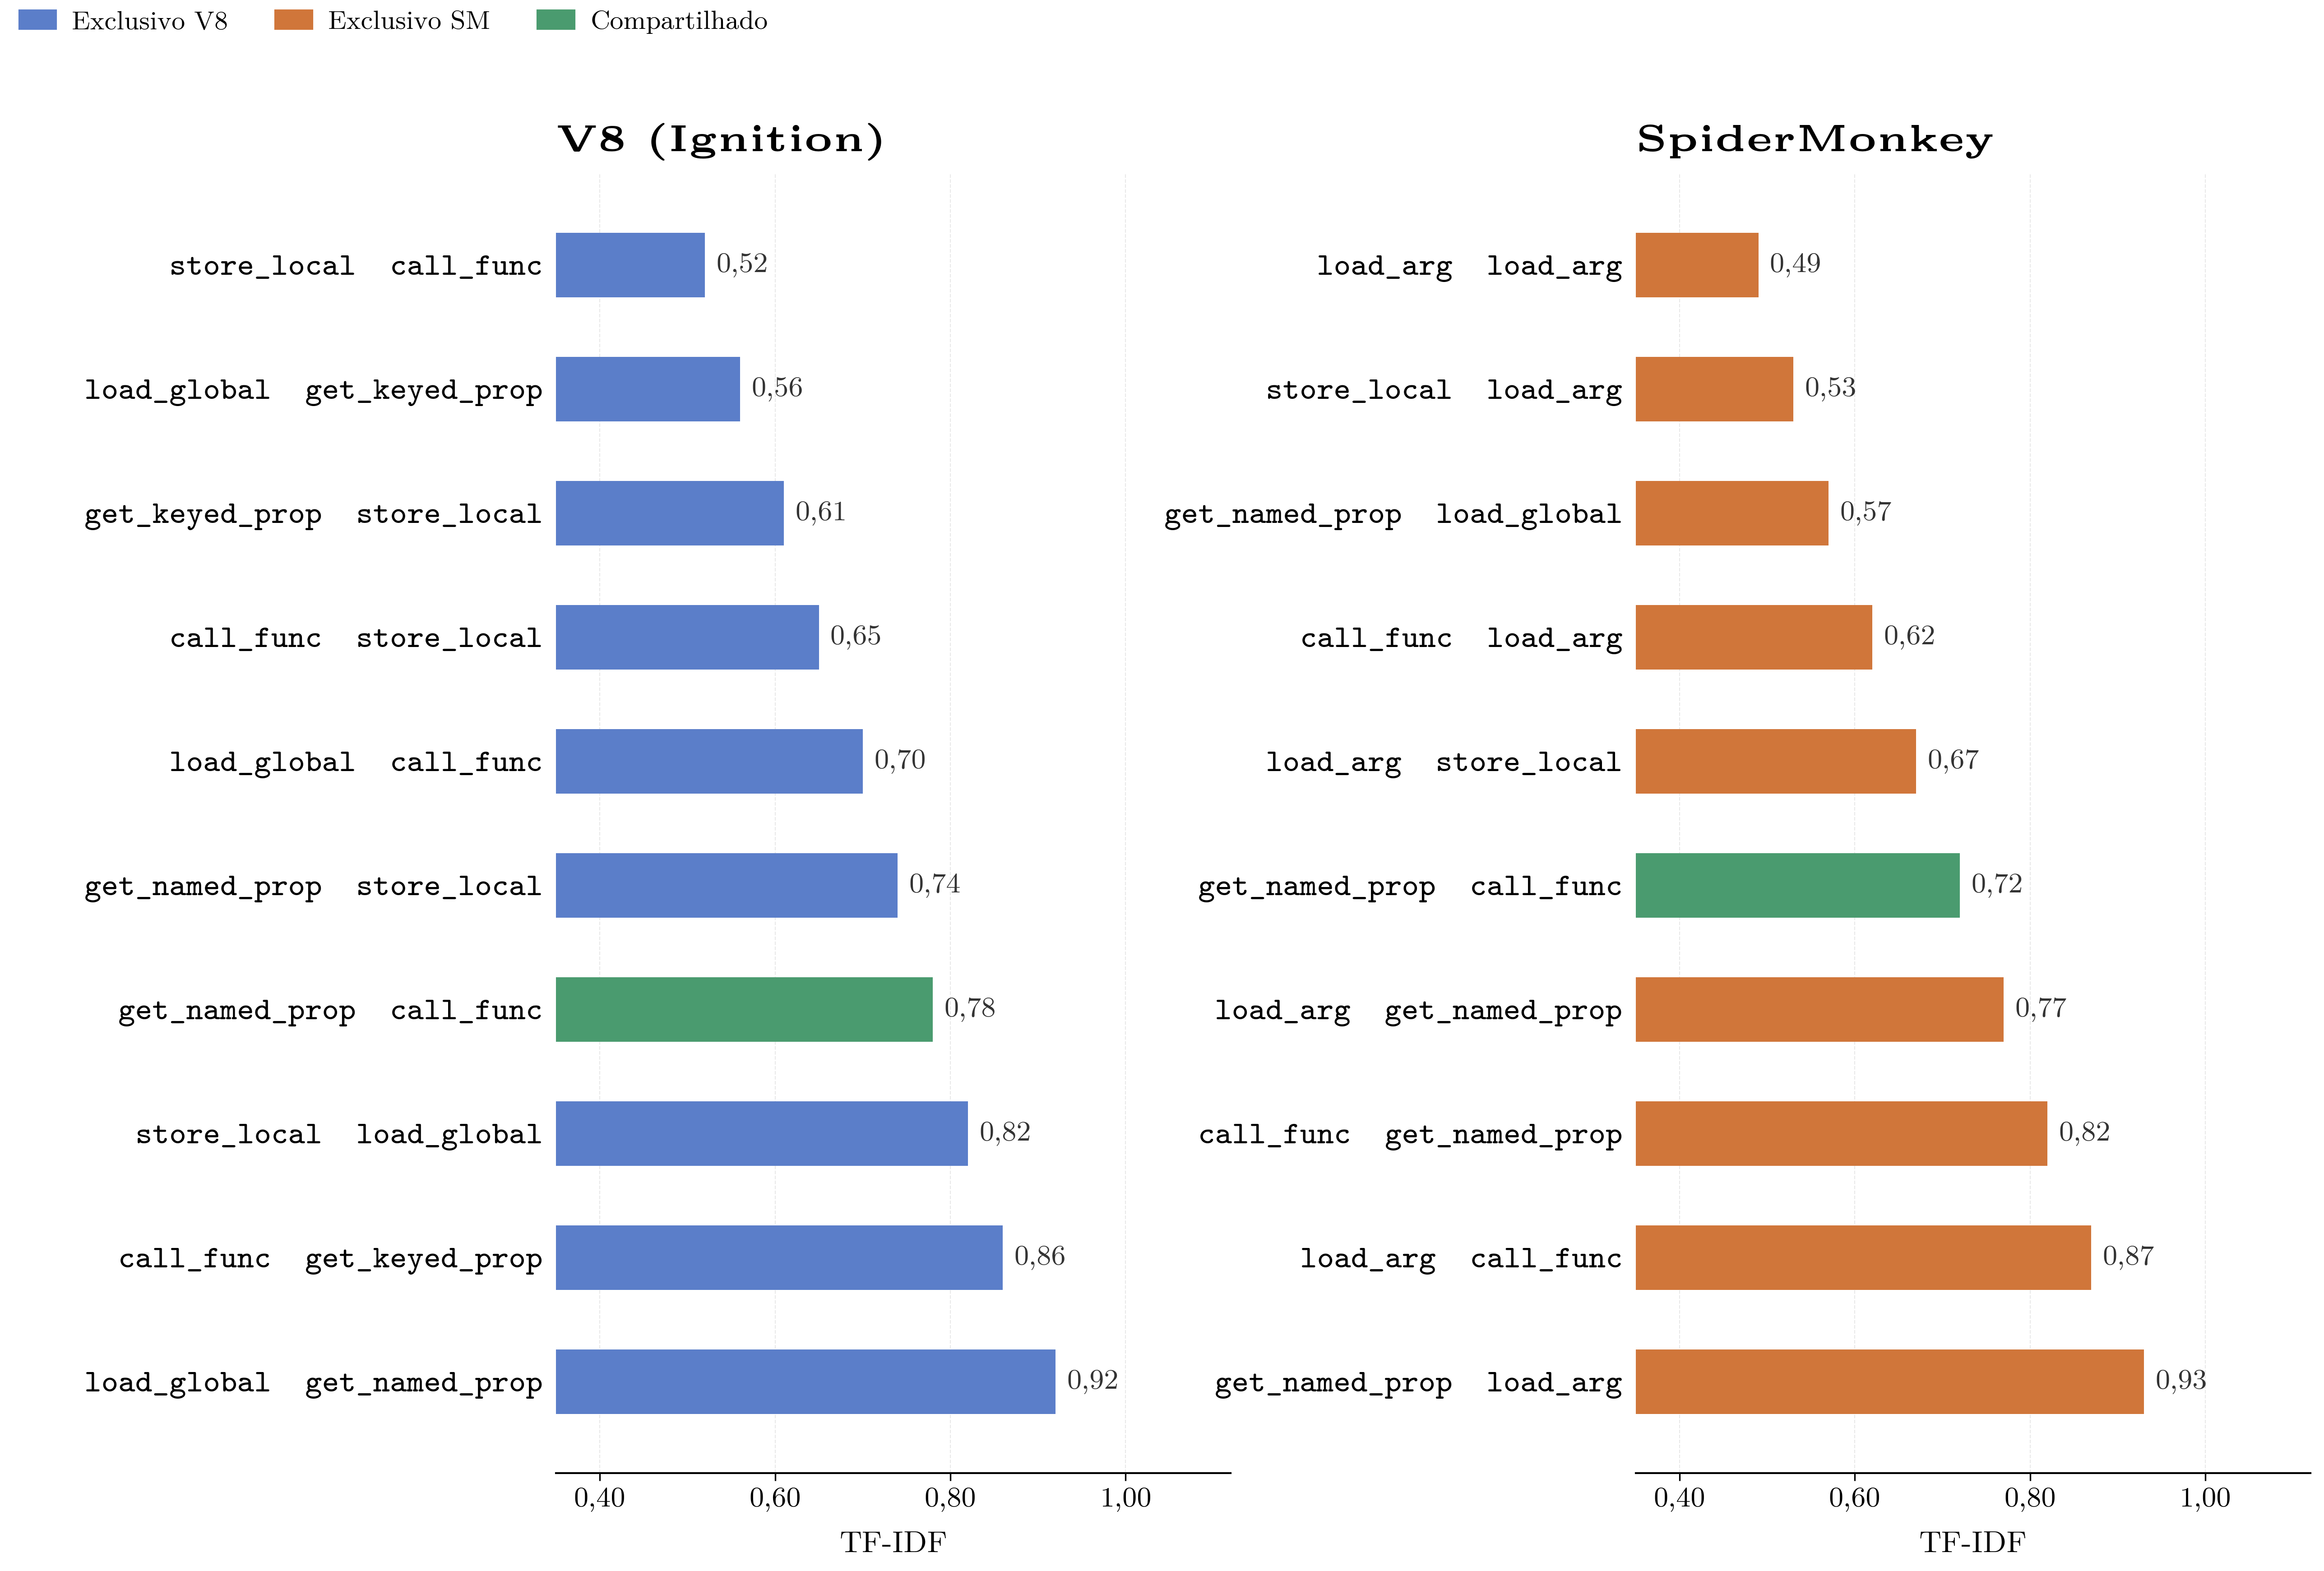
\includegraphics[width=0.88\linewidth]{fig_zeroshot_vs_joint}
\fonte{Elaborada pelo autor.}
\end{figure}

O treinamento conjunto resolve o problema ao expor o modelo às duas distribuições
simultaneamente durante o treinamento. O vocabulário compartilhado da RI garante
que os mesmos nomes de features indexem frequências comparáveis em ambos os
corpora; o modelo aprende uma superfície de decisão que generaliza sobre as duas
distribuições. O resultado (Tabela~\ref{tab:conjunto}) é um único conjunto de pesos
que atinge F1~=~0,877 no Chromium e F1~=~0,847 no Firefox com o modelo de bigrams
básico, ou F1~=~0,903 e F1~=~0,904 quando aumentado pelas features de contexto
iterativo (Tabela~\ref{tab:conjunto-iter}).

A implicação para extensibilidade é direta. Adicionar suporte a um terceiro motor
por exemplo, JavaScriptCore (Safari), exigiria: (i) instrumentar o
JavaScriptCore para emitir bytecodes; (ii) estender o dicionário de equivalência
com mapeamentos para os opcodes do novo motor, preservando os 145 tokens do dicionário de equivalência (136 ativos no TF-IDF);
e (iii) retreinar o modelo conjunto incluindo dados do terceiro motor. Não seria
necessário criar um modelo separado nem modificar os classificadores dos motores
existentes.

%, , , , , , , , , , , , , , , , , , , --
\section{Custo da independência de motor: comparação com ByteDefender}
\label{sec:disc-bytedefender}

O ByteDefender \cite{nikkhahbahrami2025} reportou F1~$\approx$~0,950 usando
bytecodes brutos do V8 em um corpus de motor único. Este trabalho atinge
F1~=~0,904 usando a RI cross-engine num corpus misto V8 + SpiderMonkey. A
diferença de \textbf{$\approx$5 pontos de F1} existe, mas os dois sistemas não
resolvem o mesmo problema: a tarefa deste trabalho é estritamente mais difícil
em três eixos.

\textbf{Funções anônimas e lambda incluídas.} O ByteDefender operou sobre funções
nomeadas, diretamente identificáveis nos metadados de bytecodes. Este trabalho
rastreia funções anônimas injetando IDs únicos em tempo de compilação (injeção de
\texttt{displayName} no SpiderMonkey; correspondência por posição no Chromium),
capturando funções cujos bytecodes não carregam nenhum sinal derivado do nome.
Funções anônimas representam uma parcela significativa do dataset; suas sequências
de bytecodes são genericamente indistinguíveis de closures utilitárias
comuns.

\textbf{Sete categorias de fingerprinting, não quatro.} O ByteDefender
cobriu canvas, fonte, áudio e WebRTC. Este trabalho inclui adicionalmente WebGL,
tela e navigator, categorias que tendem a aparecer em funções menores e
estruturalmente mais genéricas, aumentando a proporção de positivos difíceis no
dataset.

\textbf{Nenhum metadado como feature.} Apenas sequências de tokens de RI são
usadas, sem nomes de funções, URLs de script ou qualquer identificador de
contexto. O conjunto de features do ByteDefender não é completamente especificado
no artigo, mas nomes de funções como \texttt{getCanvasFingerprint} ou
\texttt{collectAudioContext} são metadados trivialmente discriminativos que
inflariam o F1 substancialmente se incluídos. A exclusão deliberada desses sinais
produz um classificador intrinsecamente robusto à renomeação de funções e à
minificação, condições comuns em bundles de produção.

Diante dessas três diferenças, a diferença de $\approx$5 pontos deve ser
interpretada como o \textbf{custo combinado da independência de motor, da inclusão
de funções anônimas, de um espaço de rótulos mais amplo e de um espaço de features
sem metadados}, não como deficiência da abordagem cross-engine.

Três fatores técnicos também contribuem para a diferença.

\textbf{Perda por abstração da RI.} O conjunto de opcodes brutos do V8 contém 198
instruções distintas mapeadas no dicionário; a RI as colapsa em 145 tokens (136 ativos
no TF-IDF após descarte de tokens raros e dos dois nunca observados no corpus).
Cada fusão descarta distinções que o modelo de motor único do ByteDefender pôde
explorar. A cobertura de 99,82\% significa que quase nenhum token é perdido, mas
muitos são agrupados, e esses agrupamentos apagam distinções discriminativas no
contexto de motor único.

\textbf{Ruído distribucional do corpus conjunto.} Para a mesma construção
JavaScript, V8 e SpiderMonkey geram padrões de n-grams distintos sob a mesma RI.
O modelo conjunto deve aprender uma superfície de decisão que satisfaça
simultaneamente ambas as distribuições, um problema estritamente mais difícil do
que ajustar uma única distribuição.

\textbf{Composição do dataset.} O dataset deste trabalho apresenta taxa de
positivos de 0,055\% nos 10.000 sites mais populares da lista Tranco, com 37.644
funções FP em 68 milhões de funções totais. A composição do dataset do ByteDefender
seleção de sites, profundidade de crawl e taxa de positivos, não foi
divulgada publicamente.

Apesar do gap, a perspectiva prática favorece a portabilidade. Com a inferência
iterativa (iter.~3, Seção~\ref{sec:iterativo}), este trabalho atinge
F1~=~0,904 no conjunto combinado V8 + SpiderMonkey sem retreinamento por motor.
Com contexto iterativo, o modelo conjunto atinge F1~=~0,903 no Chromium e
F1~=~0,904 no Firefox em avaliação por motor separada, a $\approx$0,047 do
ByteDefender, sem retreinamento por motor. A
Tabela~\ref{tab:bytedefender} sintetiza o posicionamento comparativo.

\begin{table}[htb]
\centering
\caption{Comparação com ByteDefender}
\label{tab:bytedefender}
\begin{tabularx}{\linewidth}{l>{\raggedright\arraybackslash}X>{\raggedright\arraybackslash}X}
\toprule
\textbf{Propriedade} & \textbf{ByteDefender} & \textbf{Este trabalho} \\
\midrule
Motores suportados                & V8 (Chromium)   & V8 + SpiderMonkey \\
Funções anônimas/lambda           & Não             & Sim (ID injetado em tempo de compilação) \\
Categorias de fingerprinting      & 4               & 7 \\
Features utilizadas               & Bytecodes brutos V8 & RI cross-engine (145 tokens, 136 ativos) \\
Melhor F1 binário (implantável)   & $\approx$0,950  & \textbf{0,904} (LightGBM + contexto iterativo, iter.\ 3) \\
Melhor F1 binário (limite oracle) & $\approx$0,950  & \textbf{0,928} (LightGBM + contexto de script real) \\
F1 no Chromium$\star$              & $\approx$0,950  & \textbf{0,903} (modelo conjunto + contexto iterativo) \\
F1 no Firefox (modelo conjunto)   & ---             & \textbf{0,904} (com contexto iterativo) \\
Retreinamento para novo motor     & Obrigatório     & Não necessário \\
Tamanho do modelo recomendado     & -               & 7,1~MB (LightGBM + TF-IDF) \\
\bottomrule
\end{tabularx}
{\footnotesize $\star$ByteDefender opera exclusivamente no Chromium (motor único, sem modelo conjunto);
o valor $\approx$0,950 é do modelo de motor único. O valor 0,903 deste trabalho é do modelo conjunto V8+SM.}

\fonte{Elaborada pelo autor.}
\end{table}

Para um detector implantado num ecossistema heterogêneo de navegadores, a
eliminação do retreinamento por motor representa uma redução substancial de esforço
de engenharia. O custo de $\approx$5 pontos de F1 é o preço mensurável dessa
portabilidade, considerando uma tarefa de classificação estritamente mais difícil.

%, , , , , , , , , , , , , , , , , , , --
\section{Limites do multilabel para rótulos raros}
\label{sec:disc-raro}

A tarefa multilabel expõe uma dificuldade que a tarefa binária obscurece: as sete
categorias de fingerprinting não têm suporte comparável no dataset, e a
assimetria entre a mais comum (Tela: 24.939 funções FP) e as mais raras (WebRTC:
180; Fonte: 208) abrange aproximadamente duas ordens de magnitude (razão $\approx$138:1). Esse nível de escassez interage
de formas distintas com cada família de modelos. O LightGBM com balanceamento automático de classes colapsa nos rótulos raros:
o classificador WebRTC prediz positivo para quase toda função testada, obtendo
P~=~0,0007 e F1~=~0,001 --- a heurística foi projetada para o regime de
desbalanceamento binário simples e sobre-corrige com apenas 39 positivos contra
$\approx$105.123 negativos no conjunto de teste (105.162 instâncias totais menos
39 positivos WebRTC).
O Transformer com Focal Loss também não converge para os rótulos raros dentro
do budget de treinamento testado, com apenas 39 positivos de teste por rótulo raro
(WebRTC e Fonte; os conjuntos de treino correspondentes têm $\approx$144 e
$\approx$166 positivos respectivamente, ainda insuficientes para os rótulos raros).

O RF com \texttt{balanced\_subsample} tolera melhor a escassez porque o balanceamento
opera no nível da árvore individual: cada árvore vê uma visão balanceada de seus
dados de bootstrap, mas o ensemble não adota um limiar de decisão extremo. Os
classificadores WebRTC e Fonte produzem F1~=~0,201 e F1~=~0,345, baixos, mas não
degenerados. Para os rótulos bem suportados (Tela, WebGL, Navigator e Canvas), todos
os três modelos produzem F1 acima de 0,68, confirmando que os bytecodes da RI
carregam sinal multilabel genuíno quando o suporte é adequado. O caminho mais direto
para melhorar WebRTC e Fonte é a coleta direcionada de sites conhecidos por usar
esses vetores, não melhorias no modelo. Os resultados completos estão na
Tabela~\ref{tab:multilabel}.

%, , , , , , , , , , , , , , , , , , , --
\section{Implantabilidade prática}
\label{sec:disc-implantacao}

Os resultados de latência (Tabela~\ref{tab:inferencia}) estabelecem que a detecção
cross-engine por bytecodes é praticável sem hardware especializado. Com lote de
1.000 funções, o modelo LightGBM de bigrams classifica a \textbf{44~µs por função}
em CPU de propósito geral. Uma página web típica aciona algumas centenas de funções
JavaScript durante o carregamento; a vazão de $\approx$22.700~funções/segundo
significa que o traço de bytecodes de uma página completa seria classificado em
\textbf{menos de 15~ms}, imperceptível ao usuário.

O tamanho do artefato de implantação é compacto: o modelo LightGBM de bigrams
ocupa 7,0~MB serializado, mais 140~KB para o vetorizador TF-IDF, total de
$\approx$7,1~MB. Esse footprint é adequado para inclusão em extensões de
navegador, proxies de rede ou pipelines de análise pós-crawl.

Três cenários de implantação são viáveis com os artefatos produzidos:

\textbf{Extensão de navegador em tempo real.} O content script já
instrumentado (Capítulo~\ref{cap:arquitetura}) pode ser estendido para enviar
bytecodes capturados para um serviço local ou embutir o modelo TF-IDF + LightGBM
diretamente em WebAssembly. A latência de 44~µs por função a lotes de 1.000 é
compatível com análise em tempo real durante o carregamento da página.

\textbf{Proxy de rede ou gateway de segurança.} Um proxy que intercepte respostas
JavaScript pode executar o modelo offline sobre bytecodes pré-compilados,
sinalizando scripts com alta densidade de funções FP detectadas antes de repassá-los
ao cliente.

\textbf{Auditoria de crawl em escala.} O pipeline completo demonstrou
viabilidade em escala de 68 milhões de funções; o processamento pós-crawl é
o caso de uso de menor latência exigida e maior throughput disponível.

As limitações operacionais conhecidas do sistema são as seguintes. \textbf{Web
Workers} não são cobertos pela extensão de captura: APIs de fingerprinting
invocadas em Workers (contexto isolado) não são registradas. \textbf{Funções carregadas de forma lazy} só aparecem
nos logs de bytecodes se o navegador as compilar durante a visita; funções em
pacotes de rota que não são ativados pelo crawler são invisíveis ao pipeline.
\textbf{\texttt{eval} e \texttt{new Function}} recebem um \texttt{injected\_id}
baseado na posição da chamada \texttt{eval}, não no código gerado, o que pode
causar colisões em frameworks que geram código dinamicamente. Nenhuma dessas
limitações é específica da abordagem cross-engine proposta; todas afetam igualmente
qualquer sistema baseado em instrumentação de bytecodes.

% ============================================================
%  Capítulo 8 — Conclusão
% ============================================================
\chapter{CONCLUSÃO}
\label{cap:conclusao}

\section{Síntese das contribuições}
\label{sec:conclusao-contrib}

Este trabalho partiu de uma limitação concreta do estado da arte: o ByteDefender
\cite{nikkhahbahrami2025} demonstrou que bytecodes V8 são suficientemente
discriminativos para detectar funções de browser fingerprinting com
F1~$\approx$~0,95, mas o modelo é restrito a um único motor JavaScript e não
transfere para o Firefox/SpiderMonkey sem retreinamento completo. A questão central
investigada foi: é possível construir um único classificador que opere corretamente
em ambos os motores sem retreinamento por motor?

A resposta é afirmativa, com custo mensurável. As contribuições que sustentam essa
resposta são descritas a seguir.

\textbf{Instrumentação do SpiderMonkey com rastreamento de funções anônimas.} O
Firefox foi modificado para emitir, a cada função compilada, sua sequência de
bytecodes e metadados de identificação. O problema específico das funções anônimas
(a maioria das funções em bundles minificados) foi resolvido injetando
um identificador único como \texttt{displayName} no momento da compilação, que se
propaga para \texttt{Error.stack} e permite o join direto com as chamadas de
API capturadas pela extensão. Essa solução recuperou dados que a abordagem por
posição no código-fonte perdia em $\approx$38\% dos casos.

\textbf{Pipeline de coleta cross-engine.} Um crawler de dupla engine visita
os 10.000 sites mais populares da lista Tranco com Firefox e Chromium
instrumentados. Uma extensão de navegador compartilhada (Manifest~V3) intercepta 32
APIs de fingerprinting, normaliza propriedades exclusivas do Firefox para que
as bibliotecas de rastreamento executem o mesmo caminho de código nos dois
navegadores, e captura chamadas com resolução de frame múltiplo no call
stack. O resultado é um dataset rotulado de \textbf{68.008.403 funções JavaScript}
com 37.644 exemplos positivos de sete categorias de fingerprinting, produzido
com ambos os motores sobre o mesmo conjunto de sites.

\textbf{Representação intermediária cross-engine (contribuição principal).} Um
vocabulário de \textbf{145 tokens} (136 ativos no TF-IDF) que mapeia os opcodes nativos do V8 (198
entradas) e do SpiderMonkey (236 entradas) para uma representação compartilhada,
construído por execução pareada de 27 micro-scripts e alinhamento empírico das
sequências de bytecodes resultantes. A RI atinge \textbf{cobertura de 99,82\%} dos
tokens observados no corpus real de 68 milhões de funções, com apenas 0,18\%
mapeados para \texttt{<UNK>}. Embeddings FastText Skip-gram treinados sobre o corpus
traduzido (128 dimensões, $t=0{,}0$) apresentam coerência semântica de categoria com
gap intra/inter de +0,237.

\textbf{Avaliação comparativa de classificadores e inferência iterativa.} Cinco
famílias de modelos foram treinadas e avaliadas sobre a RI na tarefa binária
(RF, LightGBM, SVM, BiLSTM e Transformer); três dessas famílias (RF, LightGBM
e Transformer) foram também avaliadas na tarefa multilabel
(Tabela~\ref{tab:multilabel}), com a mesma divisão e as mesmas features em
todos os experimentos.
O teto de detecção baseada exclusivamente em tokens de RI (sem contexto de script)
situa-se em F1~$\approx$~0,85 (LightGBM com bigrams). O melhor
modelo sem inferência iterativa, LightGBM com bigrams e densidade de script, atinge
F1~=~0,853. A inferência iterativa, que recomputa contagens de funções
previstas em múltiplos limiares como features de contexto de script, eleva o
\textbf{resultado implantável para F1~=~0,904} sem nenhum rótulo externo. O melhor classificador multilabel, Random Forest com
\texttt{balanced\_subsample}, atinge \textbf{macro-F1~=~0,564}. Os experimentos
de transferência zero-shot confirmam que a RI é necessária mas não suficiente: o
treinamento conjunto produz um modelo com \textbf{F1~=~0,903 no Chromium e
F1~=~0,904 no Firefox} (com contexto iterativo) a partir de um único conjunto de
pesos. A diferença de
$\approx$5 pontos de F1 em relação ao ByteDefender (F1~=~0,904 vs.\
$\approx$0,950) é o custo quantificado da portabilidade entre motores, acrescido de uma tarefa estritamente mais difícil: funções anônimas incluídas,
sete categorias de fingerprinting e features exclusivamente de bytecodes
sem metadados.

As perguntas de pesquisa formuladas no Capítulo~\ref{cap:intro} são respondidas
como segue. \textbf{PQ1} (cobertura da RI $>99\%$): afirmativa, 99,82\% de
cobertura no corpus real de 68 milhões de funções. \textbf{PQ2} (detector único
cross-engine com F1 comparável ao estado da arte): afirmativa, modelo conjunto
atinge F1~=~0,903 no Chromium e F1~=~0,904 no Firefox (com contexto iterativo) sem retreinamento por motor.
\textbf{PQ3} (RI suficiente para zero-shot): negativa, transferência zero-shot
falha (F1 entre 0,149 e 0,180); treinamento conjunto é condição necessária.
\textbf{PQ4} (teto de informação): F1~$\approx$~0,85 para bytecodes puros;
F1~=~0,904 com inferência iterativa sem rótulos externos; F1~=~0,928 como limite
superior oracle.

%, , , , , , , , , , , , , , , , , , , --
\section{Limitações}
\label{sec:conclusao-limitacoes}

\textbf{Teto de informação dos bytecodes puros.} O F1~$\approx$~0,85 (F1~=~0,843
com bigrams; F1~=~0,845 com trigrams) representa o
teto para detecção baseada exclusivamente em tokens de RI sem qualquer feature de
contexto de script. O F1~=~0,853 do modelo de bigrams com densidade de script
(Tabela~\ref{tab:bin}) já incorpora um primeiro passo de contexto de
script e não é comparável ao teto de bytecodes puros. A transição de bigrams para
trigrams (+0,002~F1 com 10,7$\times$ mais features) indica que o espaço de n-grams
sobre 145 tokens está essencialmente exaurido. A inferência iterativa eleva o
resultado implantável para F1~=~0,904 incorporando contagens previstas como contexto
de script, sem consultar rótulos reais. Superar o limite superior oracle
(F1~=~0,928) requer sinais ausentes nos bytecodes: nomes de funções, contexto de
grafo de chamadas ou valores em tempo de execução.

\textbf{Rótulos raros no multilabel.} WebRTC (180 funções FP no dataset completo) e
Fonte (208) possuem suporte insuficiente para aprendizado confiável. Os melhores
resultados, F1~=~0,201 e F1~=~0,345 respectivamente, refletem a escassez de
dados, não uma limitação intrínseca da abordagem. A taxa de fingerprinting
WebRTC e de enumeração de fontes nos 10.000 sites mais populares é genuinamente
baixa.

\textbf{Cobertura de Web Workers e código lazy.} A extensão de captura não injeta
hooks em contextos de Web Worker; APIs de fingerprinting invocadas em Workers
não são registradas. Funções em pacotes de rota não ativados durante a visita do
crawler não aparecem nos logs de bytecodes.

\textbf{JavaScriptCore não instrumentado.} A RI cobre V8 e SpiderMonkey. JavaScriptCore
(Safari) não foi instrumentado; a portabilidade para um terceiro motor permanece
como hipótese de extensão, não como resultado demonstrado.

\textbf{Comparação com ByteDefender parcialmente controlada.} A composição do
dataset do ByteDefender, seleção de sites, profundidade de crawl e taxa
de positivos, não foi divulgada publicamente. O gap de $\approx$5 pontos de F1
comparando o modelo implantável (F1~=~0,904) com o ByteDefender
($\approx$0,950), inclui fatores não isoláveis além da diferença de motor,
incluindo a inclusão de funções anônimas e um espaço de rótulos mais amplo
(7 categorias vs.\ 4 do ByteDefender).

\textbf{Custo de abstração da RI não isolado.} O custo de $\approx$5 pontos de
F1 em relação ao ByteDefender é atribuído à portabilidade entre motores, mas
mistura pelo menos três fatores: (1)~perda de informação pela abstração da RI
(fusão de opcodes distintos em tokens compartilhados); (2)~ruído distribucional
do corpus conjunto (V8 e SpiderMonkey geram n-grams distintos para a mesma
construção JavaScript); e (3)~tarefa estritamente mais difícil (funções
anônimas, 7 categorias, sem metadados). Um baseline limpo para isolar o
componente~(1) seria um modelo treinado e testado \emph{no mesmo motor}, mas
sobre a RI em vez dos bytecodes brutos. Esse experimento não foi realizado; a
decomposição do custo permanece qualitativa.

%, , , , , , , , , , , , , , , , , , , --
\section{Trabalhos futuros}
\label{sec:conclusao-futuros}

\textbf{Extensão a JavaScriptCore.} A arquitetura do sistema foi projetada para
receber um terceiro motor: instrumentar o JavaScriptCore, estender o dicionário de
equivalência com os novos mapeamentos (preservando os 145 tokens existentes, 136 ativos no TF-IDF) e
retreinar o modelo conjunto. Essa extensão tornaria o sistema aplicável ao
ecossistema completo de navegadores de desktop.

\textbf{Sinais complementares para superar o teto.} A análise do
Capítulo~\ref{cap:discussao} identificou três fontes de informação que poderiam
elevar o F1 além do limite superior oracle (F1~=~0,928): nomes de funções e grafo
de chamadas, valores de propriedades em tempo de execução, e vocabulário de opcodes
mais fino (com menos fusões na RI). Uma abordagem híbrida que combine bytecodes com embeddings de nome
de função, quando disponíveis em código não minificado, é uma extensão natural.

\textbf{Coleta direcionada para rótulos raros.} WebRTC e Fonte atingiriam F1 mais
alto com suporte de treinamento adequado. Identificar e incluir sites conhecidos
por usar fingerprinting via WebRTC (ex.: serviços de videoconferência) e
enumeração de fontes (ex.: ferramentas de design web) no corpus de crawl
aumentaria o suporte positivo dessas categorias sem requerer mudanças no modelo.

\textbf{Implantação como extensão de navegador.} Os artefatos produzidos, extensão de captura de bytecodes, dicionário de RI e modelo LightGBM de 7,1~MB, são suficientes para uma prova de conceito de extensão de navegador com detecção em
tempo real. A latência de 44~µs por função é compatível com análise durante o
carregamento de página; a compilação do modelo para WebAssembly viabilizaria
execução local sem servidor.

\textbf{Análise longitudinal.} O pipeline de crawl é idempotente e
retomável. Repetir o crawl sobre os mesmos sites em intervalos regulares
permitiria rastrear a evolução das técnicas de fingerprinting ao longo do
tempo, novas APIs exploradas, mudanças em bibliotecas populares, e avaliar a
estabilidade do modelo treinado diante de concept drift.

\textbf{Web Workers.} Estender a extensão de captura para contextos de Worker (via
\texttt{ServiceWorker} e \texttt{DedicatedWorkerGlobalScope}) fecharia a lacuna de
cobertura atual e potencialmente descobriria vetores de fingerprinting não
visíveis no contexto da página principal.


% -----------------------------------------------------------
% Referências
% -----------------------------------------------------------
\bibliographystyle{abntex2-alf}
\bibliography{referencias}

% -----------------------------------------------------------
% Apêndices
% -----------------------------------------------------------
% ============================================================
%  Apêndices
% ============================================================
\appendix

% ============================================================
\chapter{DICIONÁRIO DE EQUIVALÊNCIA COMPLETO DA REPRESENTAÇÃO INTERMEDIÁRIA}
\label{ap:ir-dict}
% ============================================================

Este apêndice apresenta o dicionário de equivalência completo da representação
intermediária (RI) cross-engine. O dicionário contém 145 tokens de RI, com 198
mapeamentos de opcodes V8 (Ignition) e 236 mapeamentos de opcodes SpiderMonkey.
Tokens marcados com~$\dagger$ não aparecem no corpus real de 68~milhões de funções
e são excluídos do vocabulário TF-IDF ativo (\texttt{SCOPE\_INIT} e
\texttt{WIDE\_PREFIX}); os demais 143 tokens com pelo menos uma ocorrência reduzem-se
a \textbf{136 tokens ativos} após descarte de tokens raros pelo \texttt{min\_df}.
A coluna ``---'' indica que o motor correspondente não possui opcode equivalente
naquela categoria.

\textbf{Nota sobre tokens de chamada com aridade.} O dicionário base preserva a
separação de aridade para opcodes V8 de chamada de função: os tokens
\texttt{CALL\_FUNC\_0}, \texttt{CALL\_FUNC\_1}, \texttt{CALL\_FUNC\_2},
\texttt{CALL\_FUNC\_N}, \texttt{CALL\_METHOD\_0}, \texttt{CALL\_METHOD\_1},
\texttt{CALL\_METHOD\_2} e \texttt{CALL\_METHOD\_N} são exclusivos do V8, pois o
V8 emite opcodes distintos (\texttt{CallUndefinedReceiver0}, \texttt{CallProperty1},
etc.) conforme o número de argumentos. O SpiderMonkey não distingue aridade nesse
nível e mapeia todas as chamadas de função para \texttt{CALL\_FUNC} e
\texttt{CALL\_SUPER}/\texttt{CALL\_ITER}. A Seção~\ref{sub:aridade} descreve um
experimento que colapsa esses oito tokens V8 em dois (\texttt{CALL\_FUNC} e
\texttt{CALL\_METHOD\_N}), confirmando que a aridade não acrescenta discriminação
útil (F1 comparável com 4.623 features no modelo colapsado vs.\ 4.723 no base).

{\footnotesize
\begin{longtable}{@{}p{4.2cm}p{5.3cm}p{5.3cm}@{}}
\caption{Dicionário de equivalência da RI cross-engine (145 tokens)}
\label{tab:ap-ir-dict}\\
\toprule
\textbf{Token RI} & \textbf{V8 (Ignition)} & \textbf{SpiderMonkey} \\
\midrule
\endfirsthead
\multicolumn{3}{c}{\footnotesize(continuação)} \\
\toprule
\textbf{Token RI} & \textbf{V8 (Ignition)} & \textbf{SpiderMonkey} \\
\midrule
\endhead
\midrule
\multicolumn{3}{l}{\textit{Carregamento de literais e constantes}} \\
\midrule
\texttt{LOAD\_INT} & \texttt{LdaSmi}, \texttt{LdaZero} & \texttt{Zero}, \texttt{One}, \texttt{Int8}, \texttt{Int32}, \texttt{Uint16}, \texttt{Uint24} \\
\texttt{LOAD\_FLOAT} & --- & \texttt{Double} \\
\texttt{LOAD\_BOOL} & \texttt{LdaTrue}, \texttt{LdaFalse} & \texttt{True}, \texttt{False} \\
\texttt{LOAD\_NULL} & \texttt{LdaNull} & \texttt{Null} \\
\texttt{LOAD\_UNDEFINED} & \texttt{LdaUndefined}, \texttt{LdaTheHole} & \texttt{Undefined}, \texttt{Hole}, \texttt{Uninitialized} \\
\texttt{LOAD\_CONST} & \texttt{LdaConstant} & --- \\
\texttt{LOAD\_STR} & --- & \texttt{String} \\
\texttt{LOAD\_BIGINT} & --- & \texttt{BigInt} \\
\texttt{LOAD\_SYMBOL} & --- & \texttt{Symbol} \\
\midrule
\multicolumn{3}{l}{\textit{Variáveis locais, globais e argumentos}} \\
\midrule
\texttt{LOAD\_LOCAL} & \texttt{Ldar} & \texttt{GetLocal} \\
\texttt{STORE\_LOCAL} & \texttt{Star}, \texttt{Mov}, \texttt{Star0}--\texttt{Star15} & \texttt{SetLocal}, \texttt{InitLexical} \\
\texttt{LOAD\_GLOBAL} & \texttt{LdaGlobal}, \texttt{LdaGlobalInsideTypeof}, \texttt{LdaLookupGlobalSlot}, \texttt{LdaLookupGlobalSlotInsideTypeof} & \texttt{GetGName}, \texttt{GetName}, \texttt{GetBoundName}, \texttt{GetIntrinsic} \\
\texttt{STORE\_GLOBAL} & \texttt{StaGlobal} & \texttt{SetGName}, \texttt{StrictSetGName}, \texttt{SetName}, \texttt{StrictSetName}, \texttt{SetIntrinsic}, \texttt{InitGLexical} \\
\texttt{LOAD\_ARG} & --- & \texttt{GetArg}, \texttt{GetFrameArg}, \texttt{GetActualArg} \\
\texttt{STORE\_ARG} & --- & \texttt{SetArg} \\
\texttt{LOAD\_THIS} & --- & \texttt{FunctionThis}, \texttt{ImplicitThis} \\
\texttt{LOAD\_CALLEE} & --- & \texttt{EnvCallee}, \texttt{Callee} \\
\texttt{LOAD\_GLOBAL\_THIS} & --- & \texttt{GlobalThis}, \texttt{NonSyntacticGlobalThis} \\
\texttt{LOAD\_NEW\_TARGET} & --- & \texttt{NewTarget} \\
\texttt{LOAD\_BUILTIN} & --- & \texttt{BuiltinObject} \\
\texttt{BIND\_GLOBAL} & --- & \texttt{BindUnqualifiedGName} \\
\texttt{BIND\_NAME} & --- & \texttt{BindUnqualifiedName}, \texttt{BindName}, \texttt{BindVar} \\
\midrule
\multicolumn{3}{l}{\textit{Variáveis de closure}} \\
\midrule
\texttt{LOAD\_CLOSURE\_VAR} & \texttt{LdaContextSlot}, \texttt{LdaCurrentContextSlot}, \texttt{LdaImmutableContextSlot}, \texttt{LdaImmutableCurrentContextSlot}, \texttt{LdaContextSlotNoCell}, \texttt{LdaCurrentContextSlotNoCell}, \texttt{LdaLookupSlot}, \texttt{LdaLookupContextSlot}, \texttt{LdaLookupContextSlotNoCell}, \texttt{LdaLookupSlotInsideTypeof}, \texttt{LdaLookupContextSlotInsideTypeof}, \texttt{LdaLookupContextSlotNoCellInsideTypeof}, \texttt{LdaModuleVariable} & \texttt{GetAliasedVar}, \texttt{GetAliasedDebugVar} \\
\texttt{STORE\_CLOSURE\_VAR} & \texttt{StaContextSlot}, \texttt{StaCurrentContextSlot}, \texttt{StaContextSlotNoCell}, \texttt{StaCurrentContextSlotNoCell}, \texttt{StaLookupSlot}, \texttt{StaModuleVariable} & \texttt{SetAliasedVar}, \texttt{InitAliasedLexical} \\
\midrule
\multicolumn{3}{l}{\textit{Acesso a propriedades}} \\
\midrule
\texttt{GET\_NAMED\_PROP} & \texttt{GetNamedProperty}, \texttt{GetNamedPropertyFromSuper} & \texttt{GetProp}, \texttt{GetPropSuper} \\
\texttt{SET\_NAMED\_PROP} & \texttt{SetNamedProperty} & \texttt{SetProp}, \texttt{StrictSetProp}, \texttt{SetPropSuper}, \texttt{StrictSetPropSuper}, \texttt{SetElemSuper}, \texttt{StrictSetElemSuper} \\
\texttt{GET\_KEYED\_PROP} & \texttt{GetKeyedProperty}, \texttt{GetEnumeratedKeyedProperty} & \texttt{GetElem}, \texttt{GetElemSuper} \\
\texttt{SET\_KEYED\_PROP} & \texttt{SetKeyedProperty} & \texttt{SetElem}, \texttt{StrictSetElem} \\
\texttt{DEFINE\_OBJ\_PROP} & \texttt{DefineNamedOwnProperty} & \texttt{InitProp}, \texttt{InitHiddenProp}, \texttt{InitPropGetter}, \texttt{InitPropSetter}, \texttt{InitHiddenPropGetter}, \texttt{InitHiddenPropSetter}, \texttt{InitLockedProp}, \texttt{InitHiddenElemGetter}, \texttt{InitHiddenElemSetter} \\
\texttt{SET\_ARR\_ELEM} & \texttt{StaInArrayLiteral}, \texttt{DefineKeyedOwnProperty}, \texttt{DefineKeyedOwnPropertyInLiteral} & \texttt{InitElem}, \texttt{InitElemArray}, \texttt{InitElemInc}, \texttt{InitHiddenElem}, \texttt{InitLockedElem} \\
\texttt{SET\_PROTO} & \texttt{SetPrototypeProperties} & \texttt{MutateProto} \\
\texttt{SET\_FUN\_NAME} & --- & \texttt{SetFunName} \\
\midrule
\multicolumn{3}{l}{\textit{Operações aritméticas}} \\
\midrule
\texttt{BINARY\_ADD} & \texttt{Add}, \texttt{AddSmi}, \texttt{Add\_StringConstant\_Internalize} & \texttt{Add} \\
\texttt{BINARY\_SUB} & \texttt{Sub}, \texttt{SubSmi} & \texttt{Sub} \\
\texttt{BINARY\_MUL} & \texttt{Mul}, \texttt{MulSmi} & \texttt{Mul} \\
\texttt{BINARY\_DIV} & \texttt{Div}, \texttt{DivSmi} & \texttt{Div} \\
\texttt{BINARY\_MOD} & \texttt{Mod}, \texttt{ModSmi} & \texttt{Mod} \\
\texttt{BINARY\_POW} & \texttt{Exp}, \texttt{ExpSmi} & \texttt{Pow} \\
\midrule
\multicolumn{3}{l}{\textit{Operações bitwise}} \\
\midrule
\texttt{BIT\_OR} & \texttt{BitwiseOr}, \texttt{BitwiseOrSmi} & \texttt{BitOr} \\
\texttt{BIT\_AND} & \texttt{BitwiseAnd}, \texttt{BitwiseAndSmi} & \texttt{BitAnd} \\
\texttt{BIT\_XOR} & \texttt{BitwiseXor}, \texttt{BitwiseXorSmi} & \texttt{BitXor} \\
\texttt{BIT\_SHL} & \texttt{ShiftLeft}, \texttt{ShiftLeftSmi} & \texttt{Lsh} \\
\texttt{BIT\_SHR} & \texttt{ShiftRight}, \texttt{ShiftRightSmi} & \texttt{Rsh} \\
\texttt{BIT\_USHR} & \texttt{ShiftRightLogical}, \texttt{ShiftRightLogicalSmi} & \texttt{Ursh} \\
\midrule
\multicolumn{3}{l}{\textit{Operadores unários}} \\
\midrule
\texttt{UNARY\_NEG} & \texttt{Negate} & \texttt{Neg} \\
\texttt{UNARY\_NOT} & \texttt{LogicalNot}, \texttt{ToBooleanLogicalNot} & \texttt{Not} \\
\texttt{UNARY\_BITNOT} & \texttt{BitwiseNot} & \texttt{BitNot} \\
\texttt{INC} & \texttt{Inc} & \texttt{Inc} \\
\texttt{DEC} & \texttt{Dec} & \texttt{Dec} \\
\midrule
\multicolumn{3}{l}{\textit{Comparações}} \\
\midrule
\texttt{CMP\_EQ} & \texttt{TestEqual} & \texttt{Eq} \\
\texttt{CMP\_NEQ} & --- & \texttt{Ne} \\
\texttt{CMP\_SEQ} & \texttt{TestEqualStrict}, \texttt{TestReferenceEqual} & \texttt{StrictEq}, \texttt{StrictConstantEq} \\
\texttt{CMP\_SNEQ} & --- & \texttt{StrictNe}, \texttt{StrictConstantNe} \\
\texttt{CMP\_LT} & \texttt{TestLessThan} & \texttt{Lt} \\
\texttt{CMP\_LTE} & \texttt{TestLessThanOrEqual} & \texttt{Le} \\
\texttt{CMP\_GT} & \texttt{TestGreaterThan} & \texttt{Gt} \\
\texttt{CMP\_GTE} & \texttt{TestGreaterThanOrEqual} & \texttt{Ge} \\
\midrule
\multicolumn{3}{l}{\textit{Tipo, identidade e coerções}} \\
\midrule
\texttt{TYPEOF} & \texttt{TypeOf} & \texttt{Typeof}, \texttt{TypeofExpr} \\
\texttt{TYPEOF\_EQ} & \texttt{TestTypeOf} & \texttt{TypeofEq} \\
\texttt{INSTANCEOF} & \texttt{TestInstanceOf} & \texttt{Instanceof} \\
\texttt{IN\_OP} & \texttt{TestIn} & \texttt{HasOwn}, \texttt{In} \\
\texttt{TEST\_NULL} & \texttt{TestNull} & --- \\
\texttt{TEST\_UNDEFINED} & \texttt{TestUndefined} & --- \\
\texttt{TEST\_NULL\_OR\_UNDEFINED} & --- & \texttt{IsNullOrUndefined} \\
\texttt{TEST\_UNDETECTABLE} & \texttt{TestUndetectable} & --- \\
\texttt{TO\_NUMBER} & \texttt{ToNumber}, \texttt{ToNumeric} & \texttt{Pos}, \texttt{ToNumeric} \\
\texttt{TO\_STRING} & \texttt{ToString} & \texttt{ToString} \\
\texttt{TO\_BOOL} & \texttt{ToBoolean} & --- \\
\texttt{TO\_NAME} & \texttt{ToName} & \texttt{ToPropertyKey} \\
\texttt{TO\_OBJ} & \texttt{ToObject} & \texttt{CheckObjCoercible} \\
\midrule
\multicolumn{3}{l}{\textit{Fluxo de controle e saltos}} \\
\midrule
\texttt{JMP} & \texttt{Jump}, \texttt{JumpConstant} & \texttt{Goto} \\
\texttt{JMP\_LOOP} & \texttt{JumpLoop} & \texttt{LoopHead} \\
\texttt{JMP\_IF\_TRUE} & \texttt{JumpIfTrue}, \texttt{JumpIfTrueConstant} & \texttt{JumpIfTrue} \\
\texttt{JMP\_IF\_FALSE} & \texttt{JumpIfFalse}, \texttt{JumpIfFalseConstant} & \texttt{JumpIfFalse} \\
\texttt{JMP\_IF\_NULL} & \texttt{JumpIfNull}, \texttt{JumpIfNullConstant} & --- \\
\texttt{JMP\_IF\_NOT\_NULL} & \texttt{JumpIfNotNull}, \texttt{JumpIfNotNullConstant} & --- \\
\texttt{JMP\_IF\_UNDEFINED} & \texttt{JumpIfUndefined}, \texttt{JumpIfUndefinedConstant} & --- \\
\texttt{JMP\_IF\_NOT\_UNDEFINED} & \texttt{JumpIfNotUndefined}, \texttt{JumpIfNotUndefinedConstant} & --- \\
\texttt{JMP\_IF\_OBJ} & \texttt{JumpIfJSReceiver}, \texttt{JumpIfJSReceiverConstant} & --- \\
\texttt{JUMP\_TARGET} & --- & \texttt{JumpTarget} \\
\texttt{LOGICAL\_AND} & \texttt{JumpIfToBooleanFalse}, \texttt{JumpIfToBooleanFalseConstant} & \texttt{And} \\
\texttt{LOGICAL\_OR} & \texttt{JumpIfToBooleanTrue}, \texttt{JumpIfToBooleanTrueConstant} & \texttt{Or} \\
\texttt{LOGICAL\_NC} & \texttt{JumpIfUndefinedOrNull}, \texttt{JumpIfUndefinedOrNullConstant} & \texttt{Coalesce} \\
\texttt{SWITCH} & \texttt{SwitchOnSmiNoFeedback} & \texttt{TableSwitch} \\
\texttt{SWITCH\_CASE} & --- & \texttt{Case} \\
\texttt{SWITCH\_DEFAULT} & --- & \texttt{Default} \\
\midrule
\multicolumn{3}{l}{\textit{Chamadas de função e método}} \\
\midrule
\texttt{CALL\_FUNC} & --- & \texttt{Call}, \texttt{CallContent}, \texttt{CallIgnoresRv}, \texttt{SpreadCall}, \texttt{SpreadEval}, \texttt{StrictSpreadEval}, \texttt{Eval}, \texttt{StrictEval}, \texttt{OptimizeSpreadCall} \\
\texttt{CALL\_FUNC\_0} & \texttt{CallUndefinedReceiver0} & --- \\
\texttt{CALL\_FUNC\_1} & \texttt{CallUndefinedReceiver1} & --- \\
\texttt{CALL\_FUNC\_2} & \texttt{CallUndefinedReceiver2} & --- \\
\texttt{CALL\_FUNC\_N} & \texttt{CallUndefinedReceiver}, \texttt{CallAnyReceiver}, \texttt{CallWithSpread} & --- \\
\texttt{CALL\_METHOD\_0} & \texttt{CallProperty0} & --- \\
\texttt{CALL\_METHOD\_1} & \texttt{CallProperty1} & --- \\
\texttt{CALL\_METHOD\_2} & \texttt{CallProperty2} & --- \\
\texttt{CALL\_METHOD\_N} & \texttt{CallProperty} & --- \\
\texttt{CALL\_NEW} & \texttt{Construct}, \texttt{ConstructWithSpread}, \texttt{ConstructForwardAllArgs}, \texttt{FindNonDefaultConstructorOrConstruct} & \texttt{New}, \texttt{SpreadNew}, \texttt{NewContent} \\
\texttt{CALL\_RUNTIME} & \texttt{CallRuntime}, \texttt{CallRuntimeForPair}, \texttt{CallJSRuntime}, \texttt{InvokeIntrinsic} & --- \\
\texttt{CALL\_SUPER} & --- & \texttt{SuperCall}, \texttt{SpreadSuperCall} \\
\texttt{CALL\_ITER} & --- & \texttt{CallIter}, \texttt{CallContentIter} \\
\midrule
\multicolumn{3}{l}{\textit{Criação de objetos e funções}} \\
\midrule
\texttt{CREATE\_OBJ} & \texttt{CreateObjectLiteral}, \texttt{CreateEmptyObjectLiteral}, \texttt{CloneObject} & \texttt{NewObject}, \texttt{NewInit}, \texttt{Object}, \texttt{ObjWithProto} \\
\texttt{CREATE\_ARR} & \texttt{CreateArrayLiteral}, \texttt{CreateEmptyArrayLiteral}, \texttt{CreateArrayFromIterable} & \texttt{NewArray} \\
\texttt{CREATE\_CLOSURE} & \texttt{CreateClosure} & \texttt{Lambda}, \texttt{FunWithProto} \\
\texttt{CREATE\_REGEXP} & \texttt{CreateRegExpLiteral} & \texttt{RegExp} \\
\texttt{CREATE\_SCOPE} & \texttt{CreateFunctionContext}, \texttt{CreateFunctionContextWithCells}, \texttt{CreateBlockContext}, \texttt{CreateCatchContext}, \texttt{CreateWithContext}, \texttt{CreateEvalContext} & \texttt{PushLexicalEnv}, \texttt{PushVarEnv}, \texttt{EnterWith}, \texttt{PushClassBodyEnv} \\
\texttt{CREATE\_ARGUMENTS} & \texttt{CreateMappedArguments}, \texttt{CreateUnmappedArguments} & \texttt{Arguments} \\
\texttt{CREATE\_REST} & \texttt{CreateRestParameter} & \texttt{Rest} \\
\texttt{GET\_ITER} & \texttt{GetIterator} & \texttt{ToAsyncIter}, \texttt{OptimizeGetIterator} \\
\texttt{GET\_TEMPLATE} & \texttt{GetTemplateObject} & \texttt{CallSiteObj} \\
\texttt{GET\_SUPER} & \texttt{GetSuperConstructor} & \texttt{SuperFun}, \texttt{SuperBase} \\
\midrule
\multicolumn{3}{l}{\textit{Exceções e verificações}} \\
\midrule
\texttt{THROW} & \texttt{Throw}, \texttt{ReThrow} & \texttt{Throw}, \texttt{ThrowMsg}, \texttt{ThrowSetConst}, \texttt{ThrowWithStack} \\
\texttt{TRY\_START} & --- & \texttt{Try} \\
\texttt{TRY\_FINALLY} & --- & \texttt{Finally} \\
\texttt{CATCH\_EXCEPTION} & --- & \texttt{Exception}, \texttt{ExceptionAndStack} \\
\texttt{SET\_EXCEPTION} & \texttt{SetPendingMessage} & --- \\
\texttt{TDZ\_CHECK} & \texttt{ThrowReferenceErrorIfHole}, \texttt{ThrowSuperNotCalledIfHole}, \texttt{ThrowSuperAlreadyCalledIfNotHole}, \texttt{ThrowIfNotSuperConstructor} & \texttt{CheckAliasedLexical}, \texttt{CheckLexical} \\
\midrule
\multicolumn{3}{l}{\textit{Escopo e iteração for-in}} \\
\midrule
\texttt{PUSH\_SCOPE} & \texttt{PushContext} & \texttt{FreshenLexicalEnv}, \texttt{RecreateLexicalEnv} \\
\texttt{POP\_SCOPE} & \texttt{PopContext} & \texttt{PopLexicalEnv}, \texttt{DebugLeaveLexicalEnv}, \texttt{LeaveWith} \\
\texttt{SCOPE\_INIT}$\dagger$ & --- & \texttt{GlobalOrEvalDeclInstantiation} \\
\texttt{FOR\_IN\_START} & \texttt{ForInEnumerate} & \texttt{Iter} \\
\texttt{FOR\_IN\_PREP} & \texttt{ForInPrepare} & --- \\
\texttt{FOR\_IN\_NEXT} & \texttt{ForInNext} & \texttt{MoreIter} \\
\texttt{FOR\_IN\_STEP} & \texttt{ForInStep} & --- \\
\texttt{FOR\_IN\_DONE} & \texttt{JumpIfForInDone}, \texttt{JumpIfForInDoneConstant} & \texttt{IsNoIter} \\
\texttt{FOR\_IN\_END} & --- & \texttt{EndIter}, \texttt{CloseIter} \\
\midrule
\multicolumn{3}{l}{\textit{Generators, async e miscelânea}} \\
\midrule
\texttt{GEN\_START} & --- & \texttt{Generator} \\
\texttt{GEN\_YIELD} & \texttt{SuspendGenerator} & \texttt{InitialYield}, \texttt{Yield}, \texttt{FinalYieldRval} \\
\texttt{GEN\_RESUME} & \texttt{ResumeGenerator}, \texttt{SwitchOnGeneratorState} & \texttt{AfterYield}, \texttt{Resume}, \texttt{ResumeKind}, \texttt{CheckResumeKind}, \texttt{IsGenClosing} \\
\texttt{ASYNC\_AWAIT} & --- & \texttt{Await}, \texttt{AsyncAwait}, \texttt{CanSkipAwait}, \texttt{MaybeExtractAwaitValue} \\
\texttt{ASYNC\_RESOLVE} & --- & \texttt{AsyncResolve} \\
\texttt{ASYNC\_REJECT} & --- & \texttt{AsyncReject} \\
\texttt{GET\_ARGS\_LEN} & --- & \texttt{ArgumentsLength} \\
\texttt{RETURN} & \texttt{Return} & \texttt{Return}, \texttt{RetRval}, \texttt{SetRval}, \texttt{GetRval} \\
\texttt{NOP} & --- & \texttt{Nop}, \texttt{Lineno}, \texttt{NopDestructuring}, \texttt{NopIsAssignOp}, \texttt{ForceInterpreter}, \texttt{TryDestructuring} \\
\texttt{POP} & --- & \texttt{Pop}, \texttt{PopN} \\
\texttt{DUP} & --- & \texttt{Dup2}, \texttt{Dup}, \texttt{DupAt} \\
\texttt{SWAP} & --- & \texttt{Swap}, \texttt{Pick}, \texttt{Unpick} \\
\texttt{IS\_CONSTRUCTING} & --- & \texttt{IsConstructing} \\
\texttt{CHECK\_THIS} & --- & \texttt{CheckThis}, \texttt{CheckThisReinit} \\
\texttt{CLASS\_CHECK} & --- & \texttt{CheckClassHeritage}, \texttt{CheckReturn}, \texttt{CheckIsObj}, \texttt{CheckPrivateField}, \texttt{NewPrivateName} \\
\texttt{INIT\_HOME} & --- & \texttt{InitHomeObject} \\
\texttt{DELETE\_PROP} & \texttt{DeletePropertyStrict}, \texttt{DeletePropertySloppy} & \texttt{DelProp}, \texttt{StrictDelProp}, \texttt{DelElem}, \texttt{StrictDelElem}, \texttt{DelName} \\
\texttt{VOID\_OP} & --- & \texttt{Void} \\
\texttt{DEBUGGER} & --- & \texttt{Debugger} \\
\texttt{IMPORT} & --- & \texttt{DynamicImport}, \texttt{ImportMeta}, \texttt{GetImport} \\
\texttt{WIDE\_PREFIX}$\dagger$ & \texttt{Wide}, \texttt{ExtraWide} & --- \\
\bottomrule
\end{longtable}
}

\noindent\footnotesize{$\dagger$ Token não observado no corpus real de 68~milhões
de funções; excluído do vocabulário TF-IDF ativo.}

% ============================================================
\chapter{DETALHES TÉCNICOS DA INSTRUMENTAÇÃO DOS MOTORES}
\label{ap:instrumentacao}
% ============================================================

Este apêndice apresenta os detalhes de implementação da instrumentação do V8 e
do SpiderMonkey, complementando a descrição conceitual do
Capítulo~\ref{cap:arquitetura}.

% -----------------------------------------------------------
\section{V8: código de instrumentação}
\label{ap:v8-code}

A instrumentação é inserida no fim da função \texttt{DoFinalizeJobImpl} em
\path{v8/src/interpreter/interpreter.cc}. O bloco a seguir mostra o cálculo do
\texttt{injected\_id} via FNV-1a de 64 bits, a extração de bytecodes e a emissão
para \texttt{stderr}.

\textbf{Identificador estável por função (FNV-1a 64 bits):}

\begin{lstlisting}[language=C++]
const std::string seed =
    "v8/" + script_url_str + "/" +
    std::to_string(start_pos) + "/" + std::to_string(end_pos);
const std::string injected_id = "fn_" + std::to_string(FNV1a64(seed));
\end{lstlisting}

\textbf{Extração de bytecodes via \texttt{BytecodeArrayIterator}:}

\begin{lstlisting}[language=C++]
std::string bytecode_sequence;
interpreter::BytecodeArrayIterator it(bytecodes);
while (!it.done()) {
    bytecode_sequence +=
        interpreter::Bytecodes::ToString(it.current_bytecode());
    bytecode_sequence += ',';
    it.Advance();
}
\end{lstlisting}

\textbf{Emissão serializada para \texttt{stderr} com mutex:}

\begin{lstlisting}[language=C++]
{
    std::lock_guard<std::mutex> lock(v8log_mutex);
    std::cerr
        << "[V8Log] {"
        << "\"injected_id\":\"" << injected_id << "\","
        << "\"script_url\":\""
        << json_escape(script_url_str) << "\","
        << "\"script_id\":"  << script_id  << ","
        << "\"start_pos\":"  << start_pos  << ","
        << "\"end_pos\":"    << end_pos    << ","
        << "\"func_name\":\""
        << json_escape(func_name_str) << "\","
        << "\"bytecodes\":\""
        << json_escape(bytecode_sequence) << "\""
        << "}\n" << std::flush;
}
\end{lstlisting}

% -----------------------------------------------------------
\section{SpiderMonkey: parser do log}
\label{ap:sm-parser}

A função \texttt{parse\_spidermonkey\_batch()} no crawler Firefox processa
o arquivo \texttt{geckodriver\_raw.log} ao final de cada batch de sites.
Os passos do parser são:

\begin{enumerate}
  \item Identifica blocos delimitados por \texttt{[SpiderMonkey Log]};
  \item Extrai os campos \texttt{Script URL}, \texttt{Internal Index},
    \texttt{Function name} e \texttt{Bytecode} de cada bloco;
  \item Descarta registros cujo \texttt{Script URL} comece com prefixos internos
    do Firefox: \texttt{resource://}, \texttt{chrome://},
    \texttt{moz-extension://}, \texttt{moz-src:}, \texttt{file:},
    \texttt{moz-nullprincipal:}, \texttt{<anonymous code>}, \texttt{about:},
    \texttt{data:};
  \item Deduplica registros via hash FNV-1a 64 bits de
    \texttt{(script\_url, func\_name)}, tanto dentro do batch corrente
    quanto em relação a batches anteriores da mesma sessão;
  \item Escreve os registros novos no arquivo
    \texttt{firefox\_sm\_bytecodes.jsonl.gz} no formato JSONL unificado.
\end{enumerate}

% ============================================================
\chapter{DETALHES DOS CRAWLERS E EXTENSÃO DE NAVEGADOR}
\label{ap:crawler-ext}
% ============================================================

Este apêndice reúne os detalhes de implementação dos crawlers Python e da
extensão de navegador compartilhada, complementando a descrição conceitual do
Capítulo~\ref{cap:arquitetura}.

% -----------------------------------------------------------
\section{Formato de emissão do SpiderMonkey}
\label{ap:sm-formato}

Cada função compilada pelo SpiderMonkey instrumentado gera um bloco de texto
no \texttt{stderr} com o seguinte formato:

\begin{lstlisting}[language={}]
[SpiderMonkey Log]
Script URL: https://example.com/bundle.js
Internal Index: 7
Function name: canvasFingerprint
Bytecode: [FunctionThis, SetLocal, Pop, GetGName, ...]
\end{lstlisting}

% -----------------------------------------------------------
\section{Padrões de hooking de protótipos na extensão}
\label{ap:ext-hook}

A interceptação de métodos é implementada via substituição direta no protótipo:

\begin{lstlisting}[language=JavaScript]
const _original = API.prototype.method;
API.prototype.method = function () {
    capture('categoria.metodo');
    return _original.apply(this, arguments);
};
\end{lstlisting}

Propriedades somente leitura (getters de \texttt{Screen} e \texttt{Navigator})
são redefinidas via \texttt{Object.defineProperty} com preservação do getter
original:

\begin{lstlisting}[language=JavaScript]
Object.defineProperty(Screen.prototype, 'colorDepth', {
    get: function () {
        capture('screen.colorDepth');
        return desc.get.call(this);
    },
    configurable: true,
});
\end{lstlisting}

% -----------------------------------------------------------
\section{Parser de stack trace e captura de pilha multi-frame}
\label{ap:ext-stack}

O parser de frames suporta os formatos de stack trace de ambos os motores:

\begin{lstlisting}[language=JavaScript]
// V8/Chrome: "    at funcName (url:line:col)"
const v8Named = frame.match(
    /at ([^(@]+)\s+\((.+):(\d+):(\d+)\)/);

// Gecko/Firefox: "funcName@url:line:col"
const geckoNamed = frame.match(
    /^([^@\s]+)@(https?:\/\/.+):(\d+):(\d+)$/);
\end{lstlisting}

Para evitar interferência de bibliotecas de fingerprinting que sobrescrevem
\texttt{Error.prepareStackTrace} (como o CreepJS), a captura preserva e restaura
o valor original antes de instanciar o \texttt{Error}:

\begin{lstlisting}[language=JavaScript]
function getRawStack() {
    const saved = Error.prepareStackTrace;
    Error.prepareStackTrace = undefined;
    const err = new Error();
    Error.prepareStackTrace = saved;
    return err.stack || '';
}
\end{lstlisting}

% -----------------------------------------------------------
\section{User-Agent de spoofing}
\label{ap:ua}

O crawler Firefox configura o User-Agent para o valor idêntico ao do
Chromium~131, garantindo que os sites sirvam o mesmo bundle JavaScript aos
dois navegadores:

\begin{lstlisting}[language={}]
Mozilla/5.0 (X11; Linux x86_64) AppleWebKit/537.36
(KHTML, like Gecko) Chrome/131.0.0.0 Safari/537.36
\end{lstlisting}


\end{document}
